%%%  Ukázkový text a dokumentace stylu pro text závěrečné (bakalářské a
%%%  diplomové) práce na KI PřF UP v Olomouci
%%%  Copyright (C) 2012 Martin Rotter, <rotter.martinos@gmail.com>
%%%  Copyright (C) 2014 Jan Outrata, <jan.outrata@upol.cz>


%%  Pro získání PDF souboru dokumentu je třeba tento zdrojový text v
%%  LaTeXu přeložit (dvakrát) programem pdfLaTeX.

%%  V případě použití programu BibLaTeX pro tvorbu seznamu literatury
%%  je poté ještě třeba spustit program Biber s parametrem jméno
%%  souboru zdrojového textu bez přípony a následně opět (dvakrát)
%%  přeložit zdrojový text programem pdfLaTeX.

%%  Postup získání Postscriptového souboru je popsán v dokumentaci.


%%  Třída dokumentu implementující styl pro závěrečnou práci. Vybrané
%%  nepovinné parametry (ostatní v dokumentaci):

%%  'master' pro sazbu diplomové práce, jinak se sází bakalářská práce

%%  'program=kód' pro Váš studijní program/obor (specializaci), kódy
%%  pro diplomovou práci 'infoi' pro Informatiku (Obecná informatika),
%%  'infui' pro Informatiku (Umělá inteligence), 'ainfpst' pro
%%  Aplikovanou informatiku (Počítačové systémy a technologie), 'uinf'
%%  pro Učitelství informatiky pro střední školy, 'binf' pro
%%  Bioinformatiku, 'inf' pro Informatiku (bez specializací) a 'ainf'
%%  pro Aplikovanou informatiku (bez specializací), jinak je výchozí
%%  ainfvs pro Aplikovanou informatiku (Vývoj software), a pro
%%  bakalářskou práci 'infoi' pro Informatiku (Obecná informatika),
%%  'itp' pro Informační technologie v prezenční formě, 'itk' pro
%%  Informační technologie v kombinované formě, 'infv' pro Informatiku
%%  pro vzdělávání, 'binf' pro Bioinfomatiku, 'inf' pro Informatiku
%%  (bez specializací), 'ainfp' pro Aplikovanou informatiku (bez
%%  specializací) v prezenční formě, 'ainfk' pro Aplikovanou
%%  informatiku (bez specializací) v kombinované formě, jinak je
%%  výchozí infpvs pro Informatiku (Programování a vývoj software)

%%  'printversion' pro sazbu verze pro tisk (nebarevné logo a odkazy,
%%  odkazy s uvedením adresy za odkazem, ne odkazy do rejstříku),
%%  jinak verze pro prohlížeč

%%  'biblatex' pro zapnutí podpory pro sazbu bibliografie pomocí
%%  BibLaTeXu, jinak je výchozí sazba v prostředí thebibliography

%%  'language=jazyk' pro jazyk práce, jazyky english pro anglický,
%%  slovak pro slovenský, jinak je výchozí czech pro český

%%  'font=sans' pro bezpatkový font (Iwona Light), jinak je výchozí
%%  serif pro patkový (Latin Modern)

%%  'figures, tables, theorems a sourcecodes' pro sazbu seznamu
%%  obrázků, tabulek, vět a zdrojových kódů, jinak při =false se
%%  nesází (u theorems a sourcecodes výchozí)

\documentclass[
  master,
%  program=ainfvs,
%  printversion,
  biblatex,
%  language=english,
%  font=sans,
  figures=true,
%  tables=false,
  theorems,
  sourcecodes,
  glossaries,
  index
]{kidiplom}

%% Informace pro úvodní strany. V jazyku práce (pokud není v komentáři
%% uvedeno česky) a anglicky. Uveďte všechny, u kterých není v
%% komentáři uvedeno, že jsou volitelné. Při neuvedení se použijí
%% výchozí texty. Text pro jiný než nastavený jazyk práce (nepovinným
%% parametrem language makra \documentclass, výchozí český) se zadává
%% použitím makra s uvedením jazyka jako nepovinného parametru.

%% Název práce, česky a anglicky. Měl by se vysázet na jeden řádek.
\title{Překladač funkcionálního programovacího jazyka na~platformě GraalVM}
\title[english]{Functional Programming Language Compiler on GraalVM Platform}

%% Volitelný podnázev práce, česky a anglicky. Měl by se vysázet na
%% jeden řádek. Výchozí je prázdný.
%% \subtitle{Ukázkový text a dokumentace stylu v \LaTeX{}u}
%% \subtitle[english]{Sample text and documentation of the \LaTeX{} style}

%% Jméno autora práce. Makro nemá nepovinný parametr pro uvedení
%% jazyka.
\author{Bc. Ivo Horák}

%% Jméno vedoucího práce (včetně titulů). Makro nemá nepovinný
%% parametr pro uvedení jazyka.
\supervisor{Mgr. Petr Krajča, Ph.D.}

%% Volitelný rok odevzdání práce. Výchozí je aktuální (kalendářní)
%% rok. Makro nemá nepovinný parametr pro uvedení jazyka.
%\yearofsubmit{\the\year}

%% Anotace práce, včetně anglické (obvykle překlad z jazyka
%% práce). Jeden odstavec!
\annotation{V~rámci diplomové práce byl vytvořen interpret jazyka Scheme na platformě Graal\-VM, který svou rychlostí ve vybraných benchmarkových testech překonává implementace jako Guile nebo Racket. Zatímco většina interpretů překládá kód do bytecode, jazyky implementované nad platformou GraalVM jsou překládány do abstraktních syntaktických stromů. Tímto bylo možné implementovat jazykové vlastnosti, jako například optimalizaci koncových volání, které JVM nepodporuje. Dále interpret podporuje interoperabilitu s~jazyky implementovanými na~platformě GraalVM, a tím umožňuje polyglotní programování.}

\annotation[english]{In this master thesis, an interpreter of Scheme language was developed on the GraalVM platform that outperforms implementations such as Guile or Racket in selected benchmarks. While most implementations compile code into bytecode, languages implemented on the GraalVM platform are transformed into abstract syntax trees. This approach makes it possible to implement language features, such as Tail Call optimization, which is not natively supported by JVM. Furthermore, the interpreter supports interoperability with languages implemented on the GraalVM platform, thereby enabling polyglot programming.}

%% Klíčová slova práce, včetně anglických. Oddělená (obvykle) středníkem.
\keywords{GraalVM; TruffleScheme; polyglotní programování; partial evaluation; Truffle}
\keywords[english]{GraalVM; TruffleScheme; polyglot programming; partial evaluation; Truffle}

%% Volitelná specifikace příloh textu práce, i anglicky. Výchozí je
%% 'elektronická data v systému katedry informatiky / electronic data
%% in system of department of computer science'.
%\supplements{nejlepší software všech dob}
%\supplements[english]{the best software of all times}

%% Volitelné poděkování. Stručné! Výchozí je prázdné. Makro nemá
%% nepovinný parametr pro uvedení jazyka.
\thanks{Chtěl bych poděkovat Mgr. Petru Krajčovi, Ph.D. za cenné rady, testování a~věcné připomínky při konzultacích a~během tvorby této diplomové práce.}

%% Cesta k souboru s bibliografií pro její sazbu pomocí BibLaTeXu
%% (zvolenou nepovinným parametrem biblatex makra
%% \documentclass). Použijte pouze při této sazbě, ne při (výchozí)
%% sazbě v prostředí thebibliography.
\bibliography{bibliografie.bib}

%% Další dodatečné styly (balíky) potřebné pro sazbu vlastního textu
%% práce.
\usepackage{lipsum}
\usepackage{longtable}
\usepackage{hyperref}

\usepackage[titles]{tocloft}
\newlistof{listing}{lol}{List of Listings}

\usepackage{minted}
\usemintedstyle{lovelace}
\setminted{autogobble,linenos,mathescape,fontsize=\footnotesize,breaklines, breaksymbolleft=\space}
\renewcommand\theFancyVerbLine{\scriptsize\arabic{FancyVerbLine}~}
\renewcommand\listingscaption{Zdrojový kód}

\renewcommand{\cftlistingpresnum}{~}
\setlength{\cftlistingindent}{0.47cm}
\setlength{\cftlistingnumwidth}{1.1cm}

\hyphenation{Graal-VM}
\hyphenation{Truffle-Scheme}
\hyphenation{Interop-Library}

\begin{document}
%% Sazba úvodních stran -- titulní, s bibliografickými údaji, s
%% anotací a klíčovými slovy, s poděkováním a prohlášením, s obsahem a
%% se seznamy obrázků, tabulek, vět a zdrojových kódů (pokud jejich
%% sazba není vypnutá).
\maketitle

%% Vlastní text závěrečné práce. Pro povinné závěry, před přílohami,
%% použijte prostředí kiconclusions. Povinná je i příloha s obsahem
%% elektronických dat.

%% -------------------------------------------------------------------

\newcommand{\BibLaTeX}{\textsc{Bib}\LaTeX}

\section{Úvod}
S~rostoucí oblibou funkcionálních jazyků vzniká stále větší množství nových jazyků, které umožňují programátorům vyvíjet rychleji a efektivněji, zejména v~oblastech webového vývoje, strojového učení nebo umělé inteligence. Obecně existují dva způsoby, jak implementovat nový interpretovaný jazyk. Buďto je vytvořen nový virtuální stroj, který je navržený přesně na míru vlastnostem daného jazyka, nebo je možné implementovat jazyk nad již existujícím virtuálním strojem. Často je volena právě druhá varianta, protože tvorba nového virtuálního stroje je velice náročná a mnoho částí (např. správa paměti) je již mnohokrát implementováno. Clojure \cite{clojure-jvm}, Scala \cite{scala-jvm} nebo Ruby \cite{ruby-jvm} lze uvést jako příklady jazyků, které jsou implementovány nad již existujícím virtuálním strojem Javy (JVM). Tento přístup však s~sebou nese i mnoho úskalí. Například JVM bylo vytvořeno pro~staticky typovaný jazyk, a proto implementace dynamicky typovaného jazyka musí obsahovat mnoho typových kontrol, což má negativní dopad na výkon interpretu daného jazyka.  


Dále je pro funkcionální jazyky například typická \textit{optimalizace koncových volání} (ang. tail call optimalization), kterou JVM v~současné době vůbec nepodporuje. To není problém pro imperativní jazyky, jako je Java, které obsahují cykly. Nicméně mnoho čistě funkcionálních jazyků nahrazuje cykly rekurzí. V~takovém případě by mohla být vyčerpána maximální velikost zásobníku a program by skončil chybou. Proto některé implementace musí dělat kompromisy. Například Clojure představil speciální klíčové slovo \texttt{recur} \cite{recur-doc}, které značí koncovou rekurzi (metoda volá sama sebe v~koncové pozici). Ta je během překladu převedena na~smyčku, čímž je eliminováno riziko vyčerpání zásobníku. Je důležité poznamenat, že Clojure tímto vyřešil jen koncovou rekurzi, což je speciální případ koncového volání. Projekt Loom by potenciálně mohl přidat nativní podporu koncového volání do JVM, ale v~době psaní diplomové práce není jisté, kdy a~v~jaké podobě bude podpora implementována \cite{project-loom}.

Všechna tato úskalí jsou řešitelná pomocí nového frameworku zvaného Truffle od společnosti Oracle, který je součástí platformy GraalVM. Jedná se o framework, který slouží pro implementaci nových jazyků nad platformou GraalVM. Ve své podstatě se jedná o sadu tříd, rozhraní a anotací, které vývojář při implementaci nového jazyka využívá. Součástí platformy je i nový serverový překladač zvaný \textit{Graal} (odtud název GraalVM), který Truffle anotacím rozumí a společně tak během JIT kompilace generují velice efektivní strojový kód. Jelikož Truffle nepřekládá kód do Java bytecode, mohou být výše zmíněná omezení JVM buďto úplně, nebo alespoň částečně odstraněny. Jazyky implementované pomocí frameworku Truffle jsou reprezentovány jako abstraktní syntaktické stromy (AST), které jsou následně interpretovány. Interpret je standardní Java aplikace překládaná do bytecode, přičemž jazyk sám do bytecode překládán není, jako je tomu v~případě JRuby nebo Scala. Během interpretace jazyka Truffle sbírá profilující data a na základě nich se optimalizují (specializují) jednotlivé uzly abstraktního syntaktického stromu. 


Hlavním úkolem vývojáře jazyka je převést zdrojový kód \textit{hostovaného jazyka} (jazyk hostovaný na platformě GraalVM, neboli jazyk, který vývojář implementuje) do abstraktního syntaktického stromu. O~správu paměti, optimalizace a~mnoho dalšího se pak stará Truffle (spolu s~GraalVM) automaticky. To je žádoucí, jelikož právě ony optimalizace jsou jedna z~nejnáročnějších částí vývoje jazyka. Další výhodou je fakt, že optimalizace jsou jazykově nezávislé, což znamená, že budoucí zlepšení jednotlivých optimalizací zlepšuje všechny jazyky implementované pomocí frameworku Truffle.  


\subsection{Motivace}
V~současné době existuje již několik jazyků implementovaných pomocí frameworku Truffle. Jazyky jako JavaScript, Python nebo Ruby jsou implementovány přímo společností Oracle, zatímco Pascal nebo SOM\footnote{SOM (Simple Object Machine) je minimalistický dialekt jazyka Smalltalk, který byl původně vyvinut pro účely výuky a výzkumu virtuálních strojů v~rámci institutu Hasso Plattner.} jsou jazyky implementované komunitou. I~přesto, že jazyky Python nebo JavaScript obsahují funkcionální prvky, v~době psaní diplomové práce neexistuje čistě funkcionální jazyk implementovaný s využitím frameworku Truffle. Výjimkou by mohl být Mumbler, minimalistický dialekt jazyka Common Lisp, jehož implementace je však příliš zjednodušená a~neefektivní \cite{mumbler}. Další nevýhodou je fakt, že implementace je 10~let stará, a~tudíž v~dnešní době téměř nepoužitelná jako demonstrační příklad implementace funkcionálního jazyka nad platformou GraalVM. Další implementací funkcionálního jazyka je TruffleClojure, která vznikla jako diplomová práce na~Univerzitě Johanna Keplera v~Linci roku 2015~\cite{truffle-clojure}. Jelikož tato práce vznikla ve~spolupráci se společností Oracle, která nepovolila zveřejnění zdrojového kódu, je těžké posoudit úplnost, rychlost a funkčnost interpretu. Podle informací, které mi byly poskytnuty zaměstnancem společnosti Oracle, Christianem Humerem, není zdrojový kód v~publikovatelné formě a interně se na něm dále nepracuje.   

V~rámci této diplomové práce byl proto vyvinut interpret jazyka Scheme, na~kterém je demonstrována implementace funkcionálních prvků jako je optimalizace koncové rekurze, optimalizace koncových volání nebo implementace maker. Zároveň bylo vyvinuto API pro práci s~dalšími jazyky podporovanými platformou GraalVM, což umožňuje tzv. \textit{polyglotní programování}.


\subsection{Cíle a rozsah práce}
Hlavním cílem diplomové práce je vytvořit interpret funkcionálního jazyka Scheme na platformě GraalVM. Vzhledem k~omezené dostupnosti aktuálních zdrojů týkajících se používání frameworku Truffle se diplomová práce soustředí na detailní popis základních principů tohoto frameworku, včetně teoretických základů a praktických ukázek použití.


\subsubsection{Podpora funkcionálních prvků}
Jelikož neexistuje žádná veřejně dostupná implementace jazyka, která by obsahovala funkcionální prvky, jako jsou například makra nebo optimalizace koncových volání, bylo cílem zjistit, zda a v~jaké podobě je možné tyto prvky implementovat. Během implementace těchto prvků byl kladen důraz na výslednou rychlost interpretu. Například výše zmíněný interpret Mumbler již triviálně implementuje optimalizaci koncových volání, ale s jejím zavedením se rychlost výrazně snížila. 


\subsubsection{Rychlost}
Jednou z~největších předností platformy GraalVM je rychlost implementovaných jazyků. Na grafu \ref{fig:performance-graph} je možné vidět porovnání rychlosti jazyků na platformě GraalVM s~ostatními implementacemi. Například JavaScript na platformě GraalVM je téměř stejně rychlý jako na enginu V8 \cite{javascript-speed-v8-engine}. Je nutné podotknout, že rychlost enginu V8 vyžadovala obrovské investice a všechny optimalizace, které překladač provádí, jsou jazykově závislé. Pokud popularita JavaScriptu upadne nebo bude nahrazen jiným jazykem (například WebAssembly je zajímavou technologií), všechny tyto investice do rychlosti nebude možné přímo použít.  

Naopak platforma GraalVM provádí optimalizace nezávislé na interpretovaném jazyku. To znamená, že přidání nové či zlepšení existující optimalizace do platformy GraalVM by se mělo dotknout všech implementovaných jazyků a~potenciálně je zrychlit. Důležité je zmínit, že optimalizace ve virtuálním stroji nevyžadují téměř žádnou změnu v~implementaci jazyka, naopak optimalizace ve~frameworku Truffle většinou jisté změny v~implementaci vyžadují.  

Proto byl během implementace jazyka Scheme kladen důraz na rychlost a~cílem bylo zjistit, jak rychlá bude implementace v~porovnání s~již existujícími implementacemi. Z~tohoto důvodu tato implementace nepodporuje REPL,\footnote{Zkratka pro Read-Eval-Print-Loop někdy také známý jako jazyková příkazová řádka (ang. language shell). Jedná se o~jednoduché prostředí pro programování, kde uživatel může napsat výraz, který je vyhodnocen a výsledek se okamžitě vrátí uživateli. \cite{repl}} jelikož primárně slouží k~rychlému prototypování, kde rychlost není důležitým faktorem.

\subsubsection{Podpora primitivních procedur a speciálních forem}
Vzhledem k~rozsahu této práce nebylo možné implementovat celou specifikaci jazyka Scheme. Byly proto implementovány jen základní primitivní procedury a~speciální formy, které jsou potřeba k~vyhodnocení vybraných benchmarků. Podrobný seznam všech podporovaných primitivních procedur a speciálních forem je k~dispozici v~kapitole \ref{chapter-scheme-on-graalvm-platform}.


\subsubsection{Podpora polyglotního programování}
Dalším cílem této práce bylo umožnit interoperabilitu s~dalšími jazyky, které jsou podporované platformou GraalVM, a tím umožnit polyglotní programování. Muselo proto být navrženo generické API, které umožní například vyhodnocovat kód cizích jazyků nebo číst vazby definované v~globálním prostředí těchto jazyků. Jelikož interoperabilita na platformě GraalVM je stále aktivní oblastí výzkumu a~velmi rychle se vyvíjí, nebyl kladen důraz na rychlost této implementace. Optimalizace rychlosti interoperability byla tedy záměrně ponechána pro potenciální budoucí zlepšení. 



\begin{figure} [h]
    \centering
    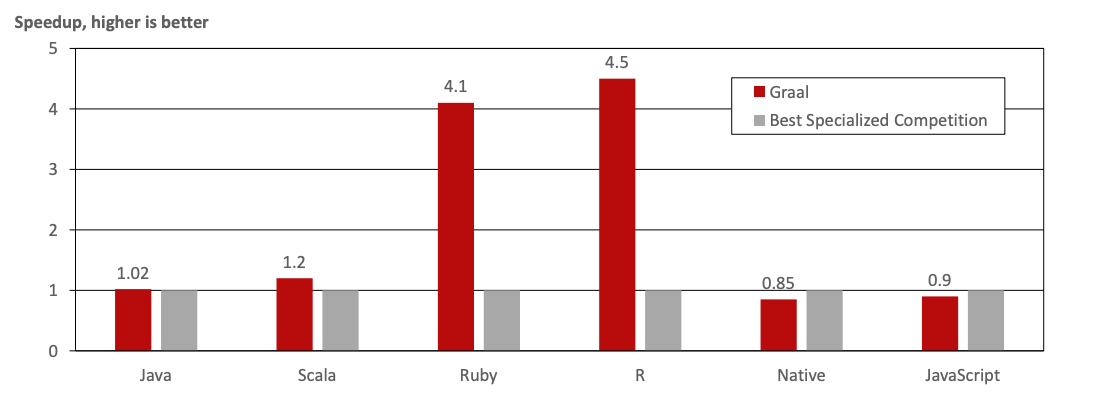
\includegraphics[width= 1\textwidth]{images/graalvm-performace-graph.png}
    \caption{Porovnání rychlosti jazyků z~roku 2017 \cite{performace-graph}}
    \label{fig:performance-graph}
\end{figure}


\clearpage

\section{Platforma Java}
Platforma Java je sada softwarových nástrojů a specifikací pro vývoj a následný běh aplikací napsaných v~jazyce Java.\footnote{V počátku byla platforma Java  primárně určena pro vývoj v~jazyce Java. V~dnešní době existuje mnoho dalších jazyků, které jsou platformou podporovány. Mezi nejznámější patří například Kotlin, Scala nebo Clojure.} Její kořeny sahají do roku 1990, kdy byla vyvinuta jako interní projekt firmy Sun Microsystems, primárně jako alternativa k~jazykům C/C++ \cite{java-platform}. Základním stavebním kamenem platformy Java je \textit{běhové prostředí} (ang. Java Runtime environment, dále JRE), které se skládá ze dvou hlavních částí:


\begin{itemize}
    \item Sada knihoven pro hladký běh aplikací (např. \texttt{rt.jar}, která obsahuje implementaci Java Core API).
    \item Virtuální stroj Javy (ang. Java Virtual Machine, dále JVM) sloužící k~interpretaci mezikódu, do kterého jsou aplikace přeloženy.  
\end{itemize}

JRE obsahuje nástroje pro běh Java aplikací, avšak nezahrnuje žádné nástroje pro vývoj, jako například debugger\footnote{Debugger je softwarový nástroj, který se používá pro hledání chyb při vývoji softwaru. \cite{debugger}} nebo překladač.\footnote{Například překladač \textit{javac} není součástí JRE, který překládá jazyk Java do bytecode.} Tyto nástroje jsou součástí Java Development Kit (dále JDK). Z~důvodu, že je JDK závislé na platformě, existují implementace pro Windows, macOS a unixové operační systémy. Schéma~\ref{fig:jdk jre jvm scheme} zachycuje vztah mezi JVM, JRE a JDK.


\begin{figure} [h]
    \centering
    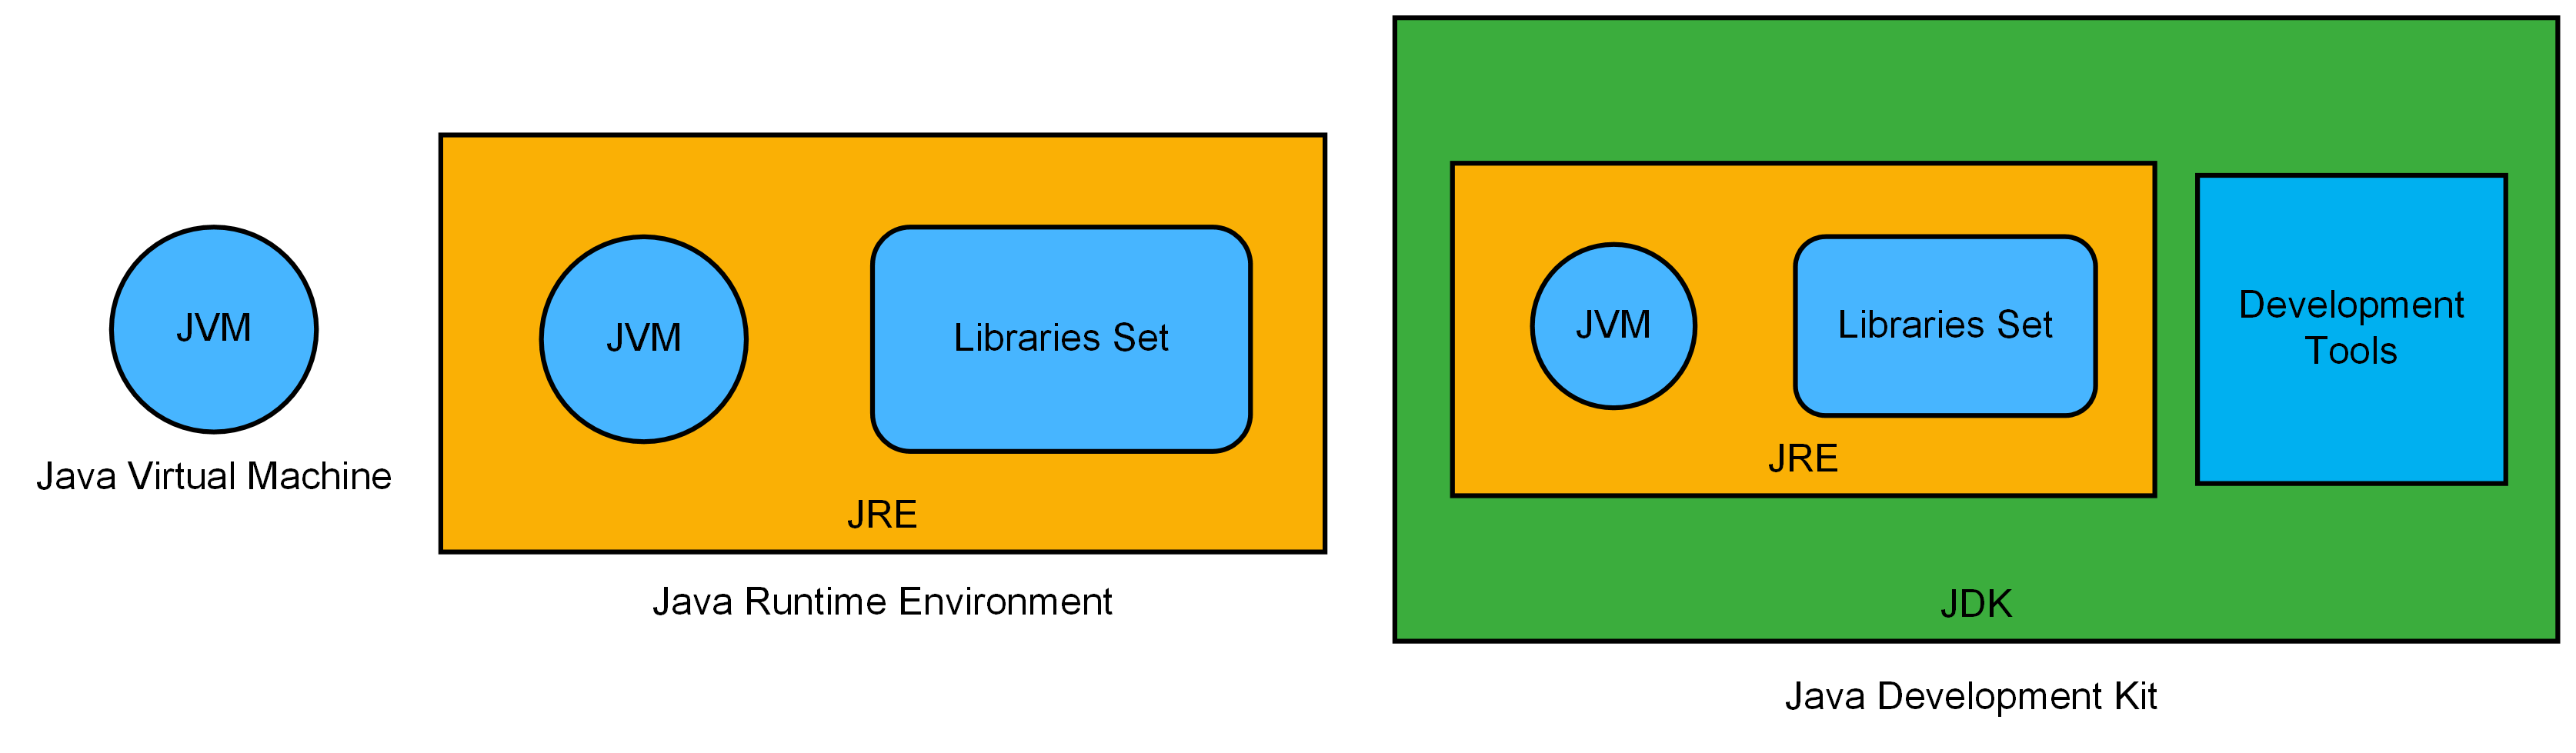
\includegraphics[width= 1\textwidth]{images/jvm-jre-jdk.png}
    \caption{Schéma znázorňující vztah mezi JDK, JRE a JVM}
    \label{fig:jdk jre jvm scheme}
\end{figure}


\subsection{Virtuální stroj Javy}
Virtuální stroj Javy je abstraktní virtuální stroj sloužící k~běhu Java aplikací. Aby aplikace mohly být spuštěny nad JVM, je potřeba je zkompilovat do tzv.~\textit{mezikódu}, který na této platformě nazýváme \textit{Java bytecode} (dále pouze bytecode). Takto zkompilovaná aplikace je uložena v~\texttt{.class} souborech, které následně interpretuje JVM. Díky tomuto přístupu je pak každá Java aplikace platformě nezávislá a jedinou limitací je přítomnost JRE na daném prostředí.  


Jednou z~nejdůležitější částí JVM je \textit{správce paměti} (ang. garbage collector), který automaticky provádí alokaci nových objektů a jejich následné uvolnění. Primárním důvodem pro automatickou správu paměti byl fakt, že téměř 70 \% chyb v~jazycích C/C++ bylo způsobeno chybnou nebo neoptimální prací s~pamětí. Existuje hned několik správců paměti (závisí na implementaci JDK), z~nichž každý je vhodný pro jiný účel (např. podle velikosti haldy). Správce paměti je pak spuštěn v~samostatném vlákně (nebo ve více vláknech), což znamená, že běží paralelně s~aplikací. Operace prováděné správcem paměti nejsou nezávislé na běhu aplikace. Například při defragmentaci haldy je nutné uzamknout některé objekty, což může ovlivnit výkon aplikace i na procesorech s~více jádry. \cite{spravce-pameti} 


Další významnou součástí JVM je \textit{interpret}, jehož hlavním úkolem je interpretovat instrukce bytecode. Jednou z~hlavních nevýhod interpretovaných jazyků je jejich nižší rychlost oproti jazykům překládaným přímo do~strojového kódu (často až desetkrát pomalejší). Tento problém byl v~pozdějších verzích Javy vyřešen využitím tzv. \textit{Just-in-time kompilace} (dále JIT kompilace). Během JIT kompilace jsou části bytecode, jako jsou funkce a bloky kódu, zkompilovány do strojového kódu a uloženy do tzv. \textit{code cache}. Takto zkompilovaný kód již není interpretován, nýbrž volán přímo z~code cache. Na obrázku \ref{fig:jit-compilation scheme} je ilustrován postup překladu jazyka Java nejprve do bytecode a poté do strojového kódu pomocí JIT kompilace. V~následující kapitole je detailně popsána JIT kompilace, včetně optimalizací, které jsou v jejím průběhu aplikovány. 


\begin{figure} [h]
    \centering
    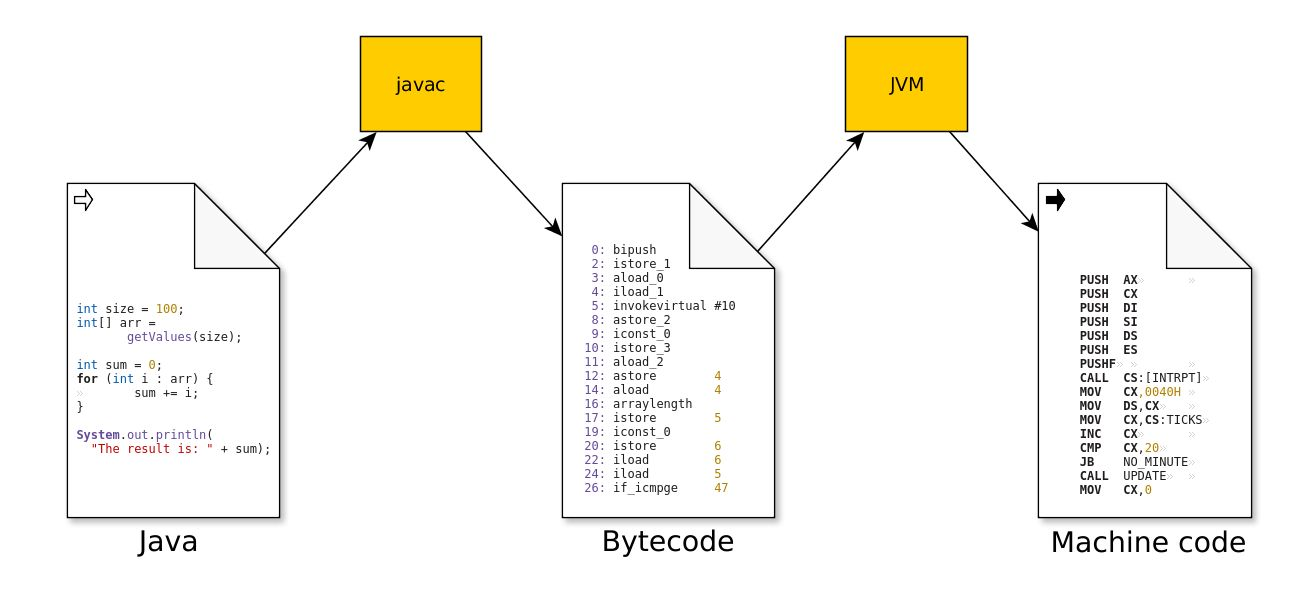
\includegraphics[width= 1\textwidth]{images/JIT-compilation scheme.jpeg}
    \caption{Příklad překladu jazyka Java do bytecode a následně do strojového kódu \cite{jit-compilation}}
    \label{fig:jit-compilation scheme}
\end{figure}



\subsection{Just-in-time kompilace}
\label{jit-compilation}
Just-in-time kompilace je technika, která kombinuje interpretaci a kompilaci kódu za účelem zvýšení výkonu aplikace. Program je nejprve interpretován a~později překládán do strojového kódu, který je uložen do code cache, odkud je volán. Jelikož code cache má omezenou velikost, nelze takto přeložit celý program. Překládají se pouze části kódu, tzv. \textit{hotspots},\footnote{Jedna z~nejznámějších implementací JVM, známá jako Hotspot JVM, odtud dostala své jméno.} které se často volají. 

Interpret při běhu programu sbírá (profiluje) data, která pak využívá pro efektivnější generování strojového kódu. Právě tato profilující data chybějí jazykům, které jsou přímo překládány do strojového kódu, a tudíž nedokážou generovat tak efektivní strojový kód. Optimalizace jsou pak často založeny na spekulacích (ang. \textit{assumptions}), kde program a jeho funkce jsou volány se specifickou konfigurací nebo s~konkrétními datovými typy. V~současných implementacích JVM jsou k~dispozici dva typy JIT překladačů, a to \textit{klient} a \textit{server}. Oba překladače jsou řízeny daty, které při běhu aplikace interpret získal. To znamená, že bytecode je na začátku relativně pomalu interpretován a až ve chvíli, kdy volání funkce nebo bloku kódu (například ve smyčce) překročí určitý práh, je kód přeložen. Mezi nejznámější prahy patří: 

\begin{itemize}
    \item \textbf{Počet volání jednotlivých metod} (ang. \textit{invocation count threshold}). Tento práh se používá pro rozhodnutí, zda metoda bude přeložena klientským nebo serverovým překladačem. 
    \item \textbf{Počet volání těla smyčky} (ang. \textit{backedge counter treshold}). Tento práh se používá pro rozhodnutí, zda tělo smyčky bude přeloženo klientským nebo serverovým překladačem.
\end{itemize}

\subsubsection{Klientský překladač}
Klientský překladač (v~implementaci Hotspot JVM nazývaný jako C1 překladač) se vyznačuje tím, že překlad provádí velice rychle a k~přeložení bytecode nepotřebuje mnoho dat z~běhu aplikace. Z~těchto vlastností vyplývá, že se primárně využívá po startu aplikace ke~zvýšení její rychlosti, jelikož při překladu provádí optimalizace daleko jednodušší a méně kvalitní v~porovnání se serverovým překladačem. Historicky se tento typ překladače používal pro aplikace, které běžely jen krátce a mezi nefunkční požadavky patřil rychlý start.

\subsubsection{Serverový překladač}
\label{server-compiler}
Serverový překladač (v~implementaci Hotspot JVM nazývaný jako C2 překladač) provádí optimalizace daleko komplexnější a často založené na spekulacích. Ty jsou nejen časově náročné, ale také je pro jejich realizaci potřeba velké množství dat z~běhu aplikace. Jedná se o~paradoxní situaci, kdy se pro dlouhotrvající aplikace vyplatí nejprve funkce nebo bloky kódu pomalu interpretovat a~jakmile jsou k~dispozici data potřebná k~překladu, je tento kód přeložen do velice efektivního strojového kódu. Jak název napovídá, tento překladač se používal pro dlouhotrvající aplikace, primárně pro serverové aplikace. \cite{spravce-pameti}

Optimalizace založené na spekulacích se mohou stát nevalidní v~případě, že některá ze spekulací již není pravdivá. V~takovém případě dochází k~tzv. \textit{deoptimalizaci}, při které je strojový kód zahozen a původní kód je opět interpretován. JVM posléze může provést opětovnou optimalizaci s~novými informacemi, které vedly k~předešlé deoptimalizaci. Tímto je zamezeno častým deoptimalizacím, které negativně ovlivňují výkon aplikace. 


\subsubsection{Vícevrstvá kompilace}
Do Javy verze 7 bylo nutné zvolit, jaký typ překladače bude aplikace využívat. Java 7 představila tzv. \textit{vícevrstvou kompilaci} (ang. tiered compilation), která využívá klientský překladač k~rychlému startu aplikace a serverový překladač k~dosažení dlouhodobě vyššího výkonu aplikace. 

\begin{figure} [h]
    \centering
    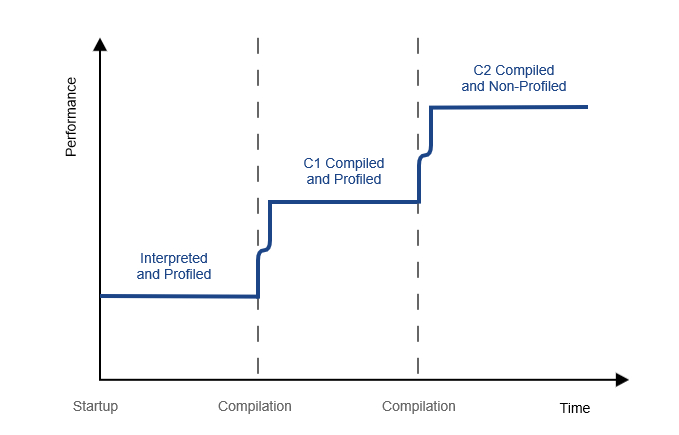
\includegraphics[width= 1\textwidth]{images/tiered-compilation.jpeg}
    \caption{Růst výkonu s~využitím vícevrstvé kompilace \cite{tiered-compilation}}
    \label{fig:tiered-compilation scheme}
\end{figure}


Obecný princip vícevrstvého překladu spočívá v~tom, že při startu aplikace je všechen bytecode interpretován a profilující data jsou použita k~nalezení často volaných funkcí/bloků kódu. Tyto často volané funkce/bloky pak JVM přeloží do strojového kódu pomocí klientského překladače, a tím se přiblíží rychlosti kompilovaných jazyků.\footnote{Rychlost bude pomalejší, protože některé části kódu jsou stále interpretovány.} Jakmile má JVM dostatek dat z~běhu aplikace, přichází na řadu serverový překladač, který provede komplexnější a déletrvající optimalizace a kód následně přeloží do strojového kódu. Takto optimalizovaný kód je pak mnohem efektivnější než strojový kód kompilovaných jazyků (C/C++).\footnote{Za předpokladu, že nedochází k~častým deoptimalizacím.} Obrázek~\ref{fig:tiered-compilation scheme} znázorňuje, jak výkon aplikace roste během jednotlivých překladů. Nutno poznamenat, že profilování se již neprovádí pouze nad interpretovaným bytecode, ale i nad strojovým kódem přeloženým klientským překladačem. Nedochází tak již k~výše zmíněné paradoxní situaci. \cite{tiered-compilation}


\subsubsection{Optimalizace realizované JIT překladači}
\label{jit-optimalizations}
Cílem této kapitoly je seznámení s~nejčastějšími optimalizacemi prováděnými klientským nebo serverovým překladačem (nebo oběma). Nejprve jsou popsány obecné oblasti, na které se JIT překladače zaměřují, a poté jsou popsány konkrétní optimalizační metody. Kapitola vychází ze zdroje \cite{optimalizace-jvm}.


\begin{enumerate}
    \item \textbf{Přístup do paměti}: Operace s pamětí jsou obecně velice pomalé. Například čtení z~operační paměti trvá přibližně 50-100ns a čtení z~registrů trvá přibližně 300ps \cite{linear-register-allocation}. Vzhledem k~tomu, že přístup k~registrům je o~tři řády rychlejší, alokace proměnných v~registrech namísto operační paměti bude klíčová pro celkový výkon. 
    \item \textbf{Volání metod}: JIT překladače využívají data z~běhu programu k~hledání často volaných metod. Volání takové metody je následně nahrazeno tělem dané metody, a tím je eliminována režie spojená s~jejím voláním. Tato optimalizace se nazývaná \textit{eliminace volání metod} (ang. method inlining).
    \item \textbf{Eliminace zámků}: JIT překladače se s~pomocí technik jako \textit{escape analysis} snaží určit, zda reference lokálních objektů neunikají mimo aktuální metodu nebo kontext. V~takovém případě se pokusí zámky buďto úplně eliminovat, nebo alespoň částečně omezit rozsah jejich platnosti.
    \item \textbf{Eliminace podmíněných skoků}: JIT překladače se snaží co nejvíce eliminovat podmíněné či nepodmíněné skoky, popřípadě kód přeskládat tak, aby prediktory skoků byly schopné odhadnout, zda se skok provede.
\end{enumerate}


\subsubsubsection{Alokace registrů}
Alokace registrů (ang. register allocation) se primárně pokouší minimalizovat přístup do operační paměti, neboť čtení z~operační paměti je výrazně pomalejší. Tento typ optimalizace implementuje jak klientský, tak i serverový JIT překladač, avšak každý využívá odlišné algoritmy. Optimální přiřazení registrů je NP-úplný problém, což znamená, že časová složitost algoritmu je exponenciální.

Většina procesorů využívá architekturu založenou na registrech, a nikoliv na zásobníku operandů (tu právě využívá JVM při interpretaci bytecode). To~znamená, že JIT překladač při překladu musí vhodně transformovat zásobníkové operandy do registrů dané procesorové architektury. Takových architektur je hned několik, například x86\_64, i686 nebo v~dnešní době čím dál populárnější ARM. To~znamená, že pro každou architekturu je nutné JIT překladače do jisté míry upravit, jelikož počet dostupných registrů a jejich využití se na každé architektuře liší. 

Klientský překladač, který je zaměřen více na rychlost překladu než na kvalitu výsledného strojového kódu, používá algoritmus nazývaný \textit{lineární alokace registrů}. Algoritmus nejprve zjistí oblasti života jednotlivých proměnných a následně se jim pokusí přiřadit registry. Pokud nastane situace, že není žádný volný registr k~dispozici, pak proměnou uloží na haldu (dochází k~tzv. \textit{variable spilling}). Tento přístup je velice rychlý, ale nejedná o~optimální řešení, a tudíž negeneruje optimální strojový kód. 


Problém přiřazení registrů lze převést na problém barvení grafu, což je algoritmus, který využívá JIT překladač typu server. Jelikož barvení grafu je opět NP-úplný problém, je tento problém řešen heuristickými (přibližnými), časově přijatelnými metodami, jejichž výsledek opět není optimální ve všech případech.

\subsubsubsection{Rozbalení programových smyček}
Jednou z~hlavních optimalizací, které eliminují podmíněné či nepodmíněné skoky, je \textit{rozbalení programových smyček} (ang. loop unrolling). Klíčovým důvodem, proč je tato optimalizace tak důležitá, je tzv. \textit{pipeline architektura}, kterou téměř všechny procesory v~dnešní době používají. Pokud se narazí na instrukci skoku, musí se nejen vyřešit problém s~rozpracovanými instrukcemi, ale i problém s~prediktivním bufferem, který se pokouší dopředu „uhodnout“, jaké instrukce budou následovat. Velmi často tento problém vyžaduje, aby všechny rozpracované instrukce byly zahozeny a pipeline se naplnila znovu. To může mít drastický dopad na výkon, kdy například Pentium 4 má pipeline rozdělenou na 30 řezů, což znamená, že se 30 instrukcí provádí paralelně a všechny tyto instrukce se musí zahodit. Z~tohoto důvodu je vhodné mít strojový kód s~co nejmenším počtem skoků, tzn. mít \textit{základní blok programu}\footnote{Základní blok programu je část programu, ve které není žádná instrukce větvení (např.~podmíněný či nepodmíněný skok, volání podprogramu nebo synchronní přerušení). \cite{zakladni-blok-programu}} co nejdelší.

JIT překladač poté využívá heuristik a dat z~běhu programu k~rozhodnutí, zda je vhodné tuto optimalizaci provést. Rozbalení každé smyčky by mohlo způsobit dramatické zvětšení velikosti výsledného strojového kódu a potenciálně by se mohl zvýšit počet tzv. \textit{cache misses}.



\subsubsubsection{Výpočet konstantních výrazů a jejich propagace}
Výpočet konstantních výrazů a jejich propagace (ang. Constant Folding and Constant Propagation) je jednou z~nejpoužívanějších optimalizačních technik. Lze ji aplikovat i na jazyky, které jsou přímo překládány do jazyka stroje. Operace, u~kterých jsou hodnoty operandů konstantní (nemění se při běhu programu), může překladač přímo vypočítat a nemusí tak pro daný výpočet generovat strojový kód. Výsledky pak mohou být dále šířeny a může docházet buďto k~dalším výpočtům konstantních výrazů anebo k~\textit{eliminaci nedosažitelného či nadbytečného kódu} (ang. dead-code elimination). Odstranění nedosažitelného kódu často vzniká při větvení, kde je podmínka konstantní, a tudíž větvení může být odstraněno. Příklad výpočtu konstantních výrazů a jejich propagace je vidět ve~zdrojovém kódu~\ref{constant-folding-and-constant-propagating}. 

\begin{listing} [H]
    \begin{minted}{java}
        // původní blok kódu před optimalizací
        int x = 14;
        int y = 7 - x / 2;
        return y * (28 / x + 2);
        
        // po propagaci proměnné x
        int x = 14;
        int y = 7 - 14 / 2;
        return y * (28 / 14 + 2);
        
        // po výpočtu konstantních výrazů a následné propagaci proměnné y
        int x = 14;
        int y = 0;
        return 0;
        
        // po odstranění zbytečného/nedosažitelného kódu
        return 0;
    \end{minted}
    \caption{Výpočet konstantních výrazů a jejich propagace}
    \label{constant-folding-and-constant-propagating}
\end{listing}


\subsubsection{Způsoby JIT kompilace}
\label{JIT-compilation-chapter}
Drtivá většina JIT překladačů je jazykově závislá, což znamená, že všechny optimalizace prováděny těmito překladači je možné dělat pouze pro jeden konkrétní jazyk nebo pro jednu konkrétní rodinu jazyků. Výborným příkladem je JavaScript, jehož výkon byl v~posledním desetiletí zlepšen o~několik řádů. Nutno podotknout, že toto zlepšení vyžadovalo obrovské investice, které jsou bohužel zřídka opodstatněné u~výzkumných projektů nebo u~doménově specifických jazyků (DSL) navržených k~řešení specifických problémů. Existují ale i techniky, které umožňují provádět jazykově nezávislé optimalizace. Jednou z~nich je \textit{meta-kompilace} (ang. meta-compilation), kterou se tato kapitola bude zabývat. 


\begin{definition} [Meta-kompilace]
\label{meta-compilation-theorem}
Meta-kompilace je výpočet, který na základě meta-systémových přechodů (ang. metasystem transitions) z~výpočetního stroje M vytvoří výpočetní stroj M', který je sémanticky totožný se strojem M \cite{metacompilation}.
\end{definition}

Jak bude možné vidět v~následujících kapitolách, meta-kompilace je pouhá transformace, která využívá data z~běhu programu a program samotný k~vytvoření nového kódu, který bude mít stejnou sémantiku jako kód původní. Meta-systémové přechody z~definice \ref{meta-compilation-theorem} odpovídají datům z~běhu programu, tzn. transformace je řízena těmito daty. Je důležité podotknout, že pokud každý program bude reprezentován stejnou strukturou (např. pomocí abstraktních syntaktických stromů), je tato transformace jazykově nezávislá. Pokud je pojem transformace nahrazen pojmem optimalizace, což je možné, jelikož jakákoliv optimalizace je pouhou transformací kódu, dostáváme pak jazykově nezávislé optimalizace. V~následujících kapitolách jsou popsány dvě nejznámější techniky meta-kompilace \textit{meta-tracing} a \textit{partial evaluation}. 


\subsubsubsection{Meta-tracing}
\label{meta-tracing-chapter}
Meta-tracing je technika meta-kompilace, jejíž základní princip spočívá ve sledování částí kódu, které byly navštíveny během vykonání programu, a jejich následné optimalizace. Jelikož sledování kódu má vliv na výkon aplikace, nesleduje se celý program, ale pouze funkce a cykly, které přesáhly práh pro JIT kompilaci. Výsledkem sledování je \textit{záznam} (ang. trace), který je optimalizován\footnote{Optimalizace jsou opět založeny na spekulacích, které vychází z~dat sesbíraných během tohoto sledování.} a poté přeložen do strojového kódu. Záznamy obsahují specifické \textit{kontroly} (ang. guards), které kontrolují, zda spekulace, které byly provedeny během optimalizací, jsou stále validní. Pokud ne, dochází ke klasické deoptimalizaci, strojový kód je zahozen a kód je interpretován. Nutno zmínit, že meta-tracing je obecná technika využívána v~různých odvětví informatiky, a proto meta-tracing popsán v~této kapitole primárně vychází z~implementace RPython, což je Python framework pro psaní interpretů. 


\begin{figure} [h]
    \centering
    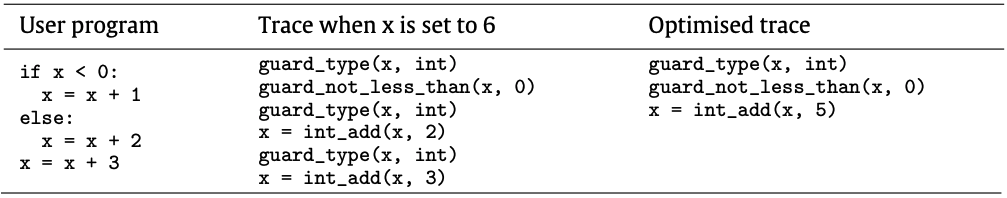
\includegraphics[width= 1\textwidth]{images/meta-tracing2.png}
    \caption{Příklad uživatelského programu (levý sloupec), jeho neoptimalizovaný záznam (sloupec uprostřed) a optimalizovaný záznam (sloupec vpravo) \cite{meta-tracing}}
    \label{fig:meta-tracking-example}
\end{figure}



Na obrázku \ref{fig:meta-tracking-example} je možné vidět uživatelský program a jeho záznamy. V~levém sloupci je uživatelský program v~jazyce Python. Pokud tento kód bude vyhodnocen jako vhodný kandidát pro JIT kompilaci (počet volání tohoto kódu překročí určitý práh), v~příštím vykonání bude kód sledován a vytvoří se záznam. Sloupec uprostřed je ukázka takového záznamu, kde při vykonávání proměnná \texttt{x} nabývala hodnoty \texttt{6}. Je důležité zdůraznit, že hodnota proměnné \texttt{x} není uložena v~záznamu. Stejný záznam by byl vytvořen pro jakoukoliv kladnou hodnotu \texttt{x}. Jakmile je záznam vytvořen, přichází na řadu jeho optimalizace, jejímž cílem je snížit velikost záznamu a vytvořit co nejefektivnější strojový kód. V~tomto případě dvě kontroly typu proměnné \texttt{x} mohou být odstraněny (jelikož typ byl ověřen hned na začátku záznamu) a poté dvě konstantní operace sčítání mohou být nahrazeny pouze jednou operací sčítání. V~pravém sloupci jsou výsledné optimalizované záznamy, které budou převedeny do strojového kódu. \cite{meta-tracing}


\subsubsubsection{Partial evaluation}
\label{partial-evaluation-chapter}
Partial evaluation je další technikou meta-kompilace, jejímž hlavním cílem je, stejně jako u~meta-tracing, transformovat kód do menší a jednodušší podoby tak, aby výsledný strojový kód byl co nejefektivnější. Základním principem této techniky je sběr dat z~běhu aplikace, která jsou použita k~vytvoření efektivnějšího kódu. Tato technika vychází z~předpokladu, že program se po určité době stane stabilním, a bude ho tudíž možné transformovat do efektivnější podoby. Tímto je možné například odstranit části původního kódu, které nejsou programem používány, nebo spekulovat nad typem argumentů u~jednotlivých funkcí. Opět je nutno zmínit, že partial evaluation je obecná technika, a proto tato kapitola vychází z~frameworku Truffle, což je Java framework pro psaní interpretů pro~libovolné jazyky nad GraalVM.



\begin{figure} [h]
    \centering
    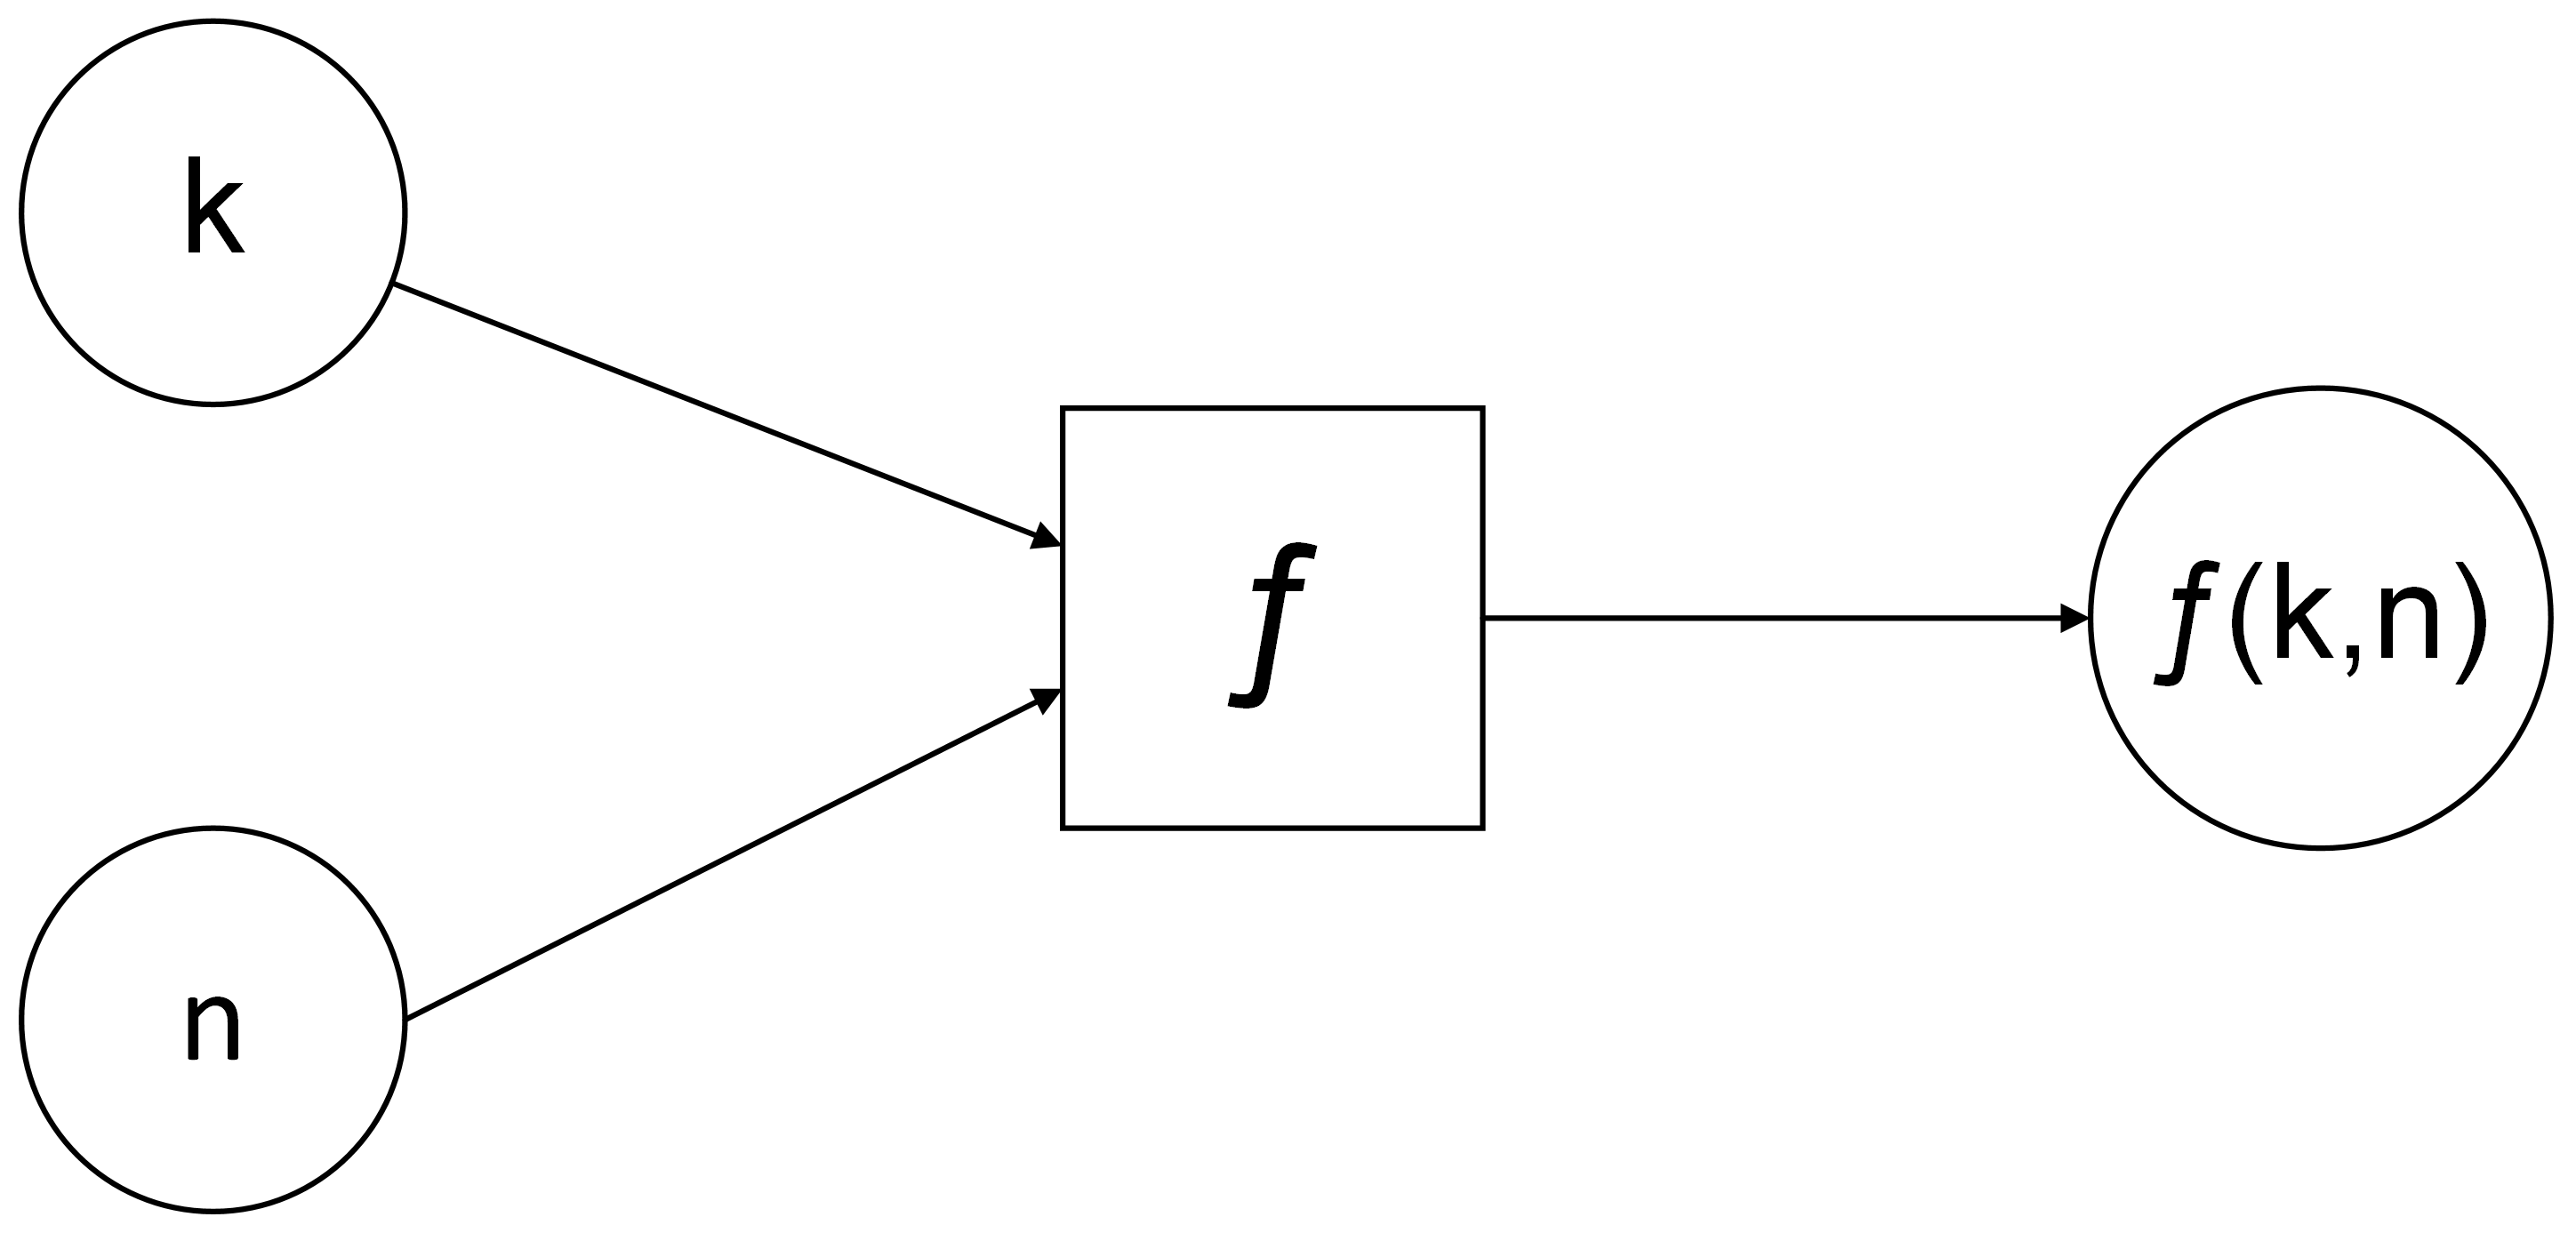
\includegraphics[width= 0.7\textwidth]{images/pow-function.png}
    \caption{Schéma funkce s~dvěma argumenty \textit{n}  a \textit{k}}
    \label{fig:pow-fucntion}
\end{figure}


Schéma \ref{fig:pow-fucntion} znázorňuje funkci \textit{f} s~dvěma argumenty \textit{n} a \textit{k}. Jak již bylo zmíněno, hlavním cílem partial evalution je transformovat funkci \textit{f} na kratší a efektivnější funkci s~využitím dat z~běhu aplikace. Řekněme, že funkce \textit{f} byla vždy volána se stejnou hodnotou argumentu \textit{k}. Jakmile JVM vyhodnotí, že funkce \textit{f} je vhodným kandidátem na JIT kompilaci, partial evaluation nejprve funkci transformuje, a~poté se transformovaný kód přeloží do strojového kódu. Schéma této transformace je znázorněno na obrázku \ref{fig:applied-PE-pow-fucntion}. Výsledkem je funkce \textit{f\textsubscript{k}}, která je sémanticky totožná s~funkcí \textit{f}. Platí proto následující vztah: \[ f(k, n) = f_{k}(n) \]

\begin{figure} [h]
    \centering
    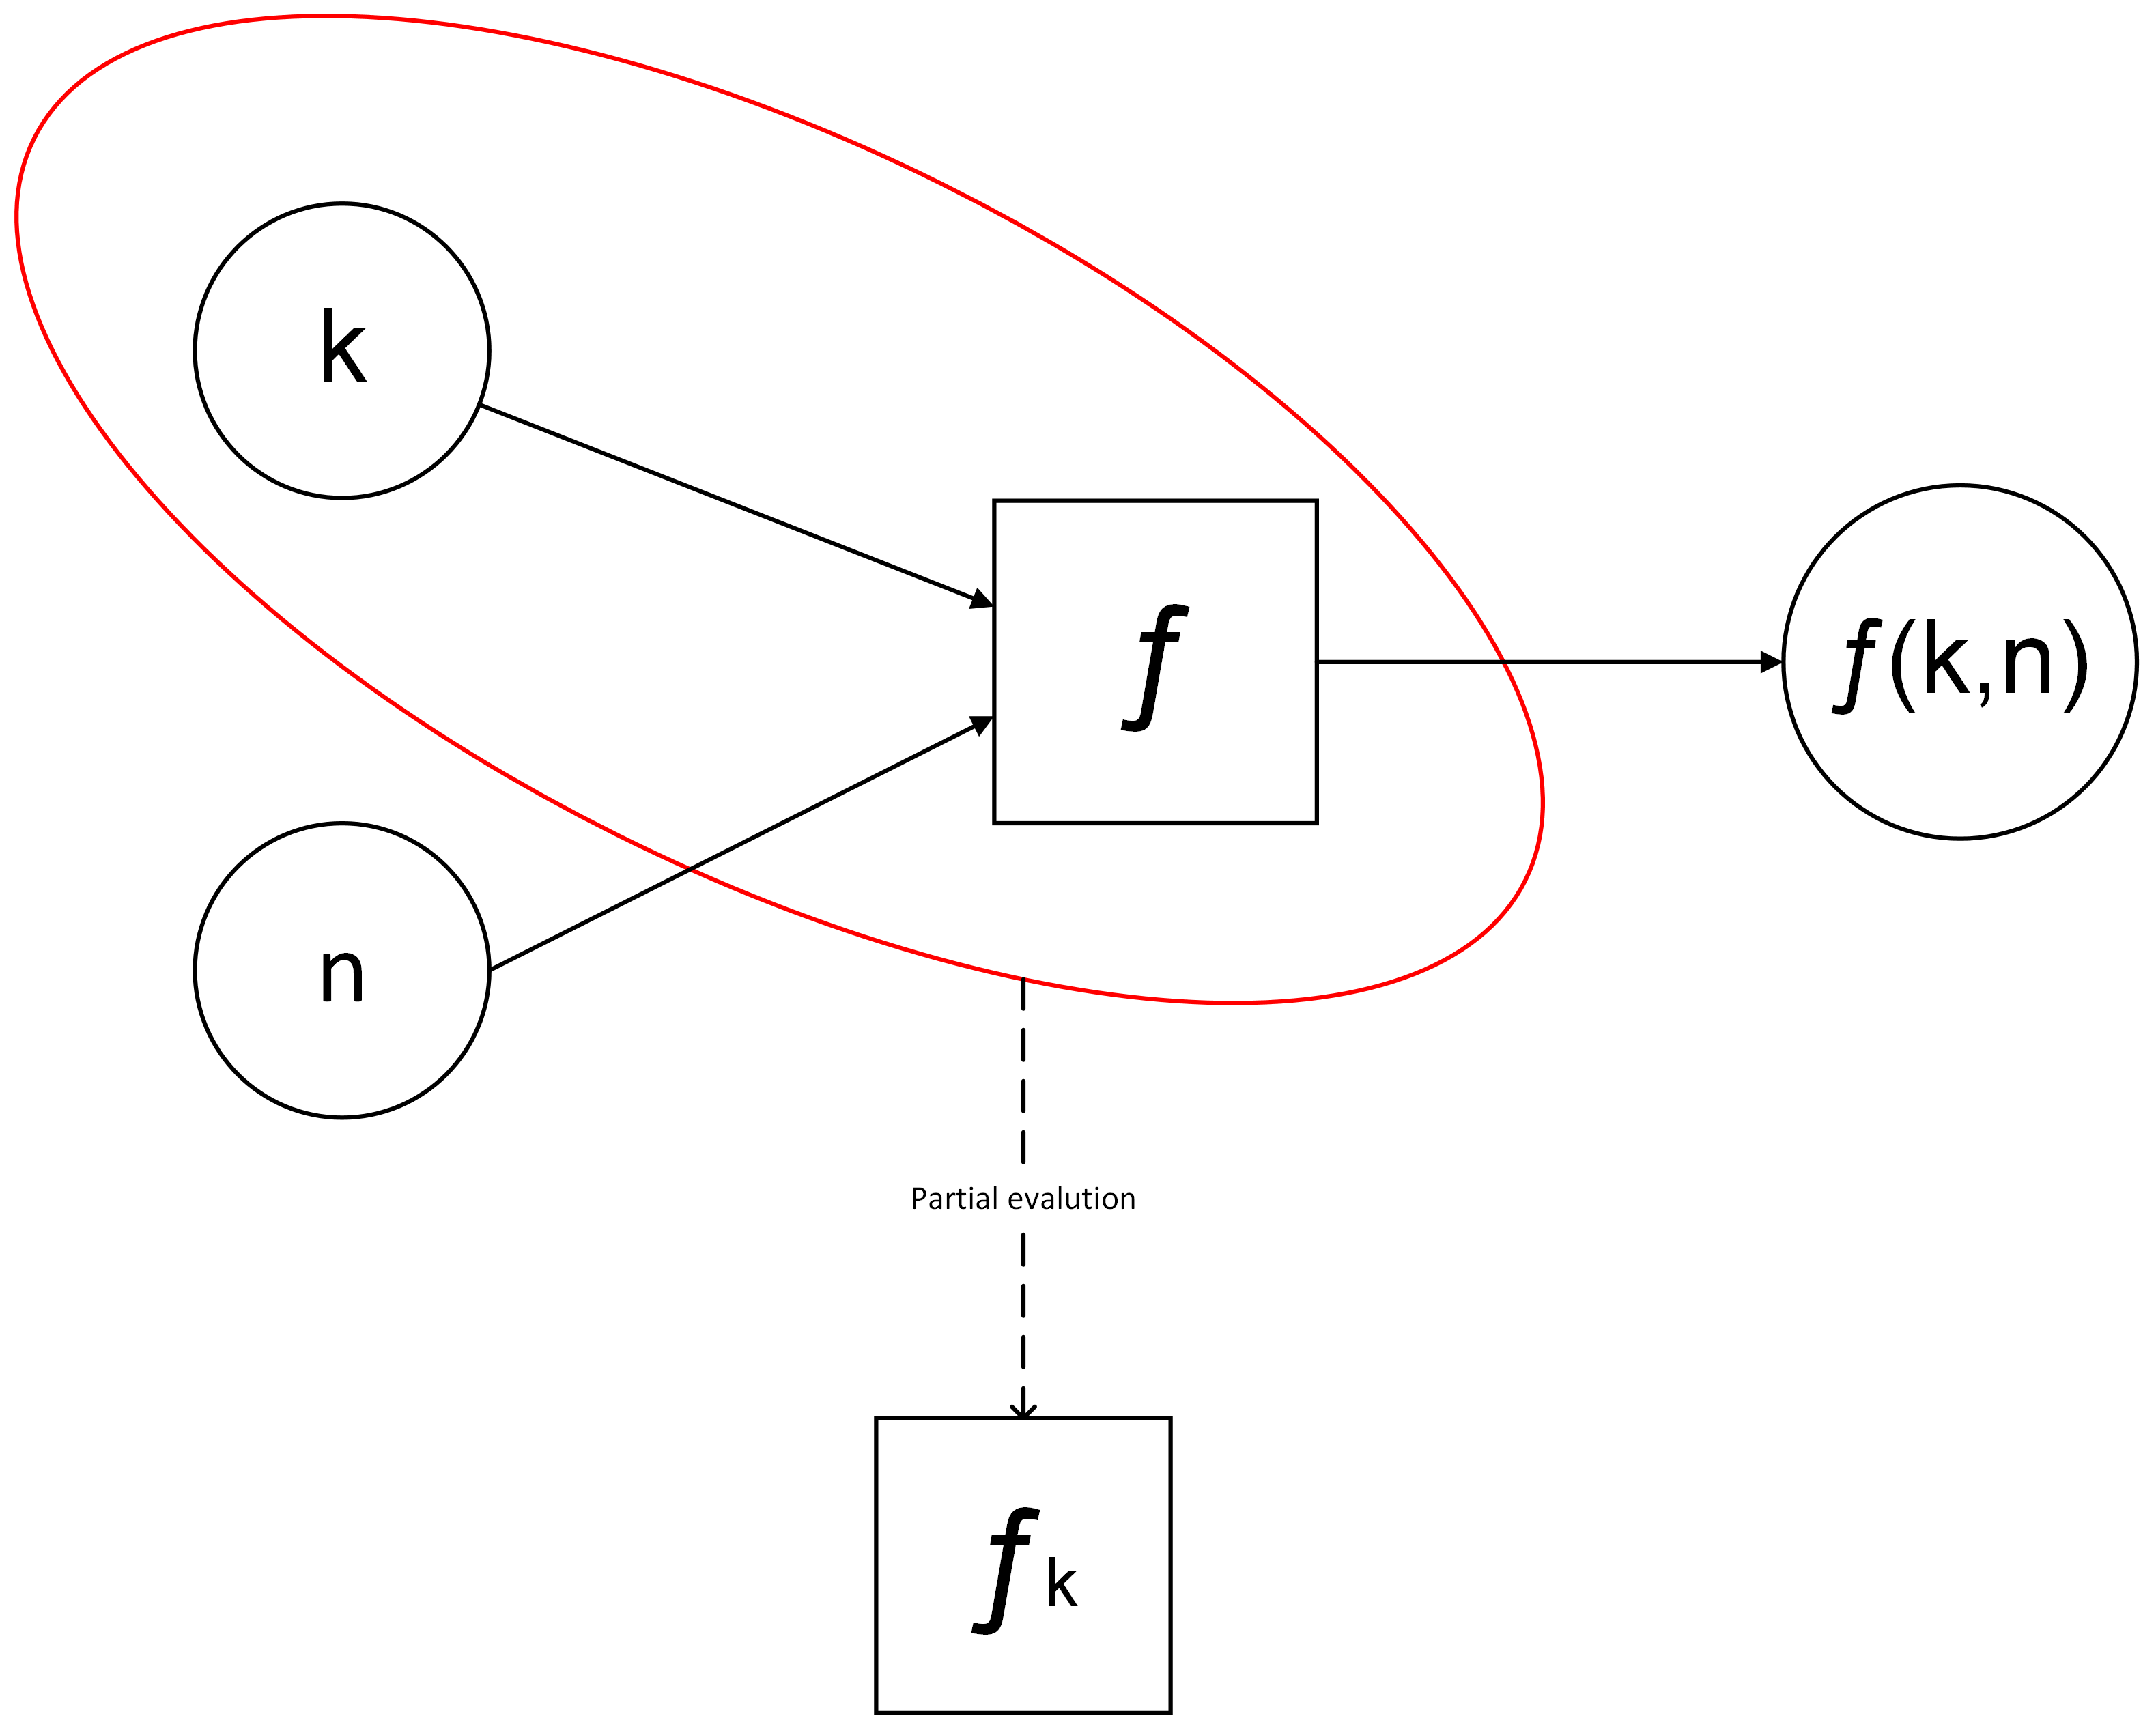
\includegraphics[width= 0.7\textwidth]{images/pow-PE.png}
    \caption{Aplikování partial evaluation na funkci \textit{f} za předpokladu, že hodnota argumentu \textit{k} je konstantní}
    \label{fig:applied-PE-pow-fucntion}
\end{figure}


Zdrojový kód \ref{partial-evaluation-example} tuto transformaci zobrazuje na konkrétní funkci \texttt{pow}. V~tomto příkladu je předpokladem, že funkce byla často volána s~hodnotou argumentu \texttt{k~=~5}. Proces partial evaluation je ve zdrojovém kódu zobrazen tak, že se postupně tvoří nové funkce \texttt{pow5}, což se ve skutečnosti samozřejmě neděje. Jak je možné vidět ze zdrojového kódu, partial evaluation s~využitím dat z~běhu (v~tomto případě je známa hodnota parametru \textit{k}) transformuje kód pomocí již výše zmíněných optimalizací. Nejprve bylo eliminováno volání metod a poté proběhlo odstranění nadbytečného kódu. V~případě, že spekulace se stane nevalidní, což znamená, že hodnota argumentu \textit{k} je jiná než 5, dojde k~deoptimalizaci a~funkce \texttt{pow} bude následně opět interpretována. 

Závěrem je nutno zmínit, že tento příklad je pouze ilustrativní a reálně by tato metoda nebyla takto transformována z~důvodu, že spekulace nad hodnotou argumentu \textit{k} je moc silná. Cílem tohoto příkladu bylo demonstrovat, že partial evaluation kód transformuje pomocí dat z~běhu programu a tvoří tak kratší a~efektivnější kód.  

\begin{listing} 
    \begin{minted}{java}
        // před transformací
        public long pow(int n, int k) {
            if (k <= 0) {
                return 1;
            } else {
                return n * pow(n, k - 1);
            }
        }
        
        // eliminace if podmínky a výpočet konstantních výrazů
        public long pow5(int n) {
            return n * pow(n, 4);
        }
    
        // eliminace funkce pow(n, 4) - vložení těla 
        public long pow5(int n) {
            return n * n * pow(n, 3);
        }
    
        ....
    
        // výsledný kód po eliminaci funkcí pow(n, 3), pow(n, 2), pow(n, 1) a pow(n, 0)
        public long pow5(int n) {
            return n * n * n * n * n * 1;
        }
        
        // odstranění nadbytečného kódu
        public long pow5(int n) {
            return n * n * n * n * n;
        }
    \end{minted}
    \caption{Partial evalution aplikovaná na funkci \texttt{pow}}
    \label{partial-evaluation-example}
\end{listing}

\clearpage

\subsubsubsection{Meta-kompilace při psaní interpretů}
Předchozí dvě kapitoly se zabývaly meta-tracing a partial evaluation jako obecnými technikami pro transformaci kódu. V~této kapitole je popsáno, jak jsou tyto techniky aplikovány při psaní interpretů. Na obrázku \ref{fig:futamura-projection} můžeme vidět klasické schéma interpretu. Interpret je program se dvěma vstupy: 

\begin{itemize}
    \item Program, který se interpretuje. 
    \item Vstupní data interpretovaného programu.
\end{itemize}

Pokud je aplikována jedna z~meta-kompilačních technik na program a interpret (znázorněno červeným kruhem na obrázku \ref{fig:futamura-projection}), vzniká nový interpret, který je přímo optimalizovaný pro vstupní program. Tato transformace se provádí za~běhu programu, a proto jsou dostupná i data z~běhu programu, která umožňují aplikovat optimalizace založené na spekulacích. Jelikož jsou během transformace aplikovány spekulace, může dojít k~situaci, kdy se spekulace stane nevalidní. V~takovém případě dochází k~deoptimalizaci a kód je interpretován. Meta-kompilační techniky tedy nezahrnují celou sémantiku daného kódu, ale pouze sémantiku, kterou interpretovaný program opravdu využívá. Výpočetní stroj \textit{M'} zmíněný v~definici \ref{meta-compilation-theorem} neobsahuje celou sémantiku stroje \textit{M}, ale obsahuje mechanismus (deoptimalizace a návrat k~interpretaci), kterým vždy celou sémantiku může pokrýt. Transformace, kdy je aplikována jedna z~meta-kompilačních technik na program a interpret, se nazývá \textit{První Futamurova projekce}, na které, jak uvidíme v~dalších kapitolách, je založen framework Truffle. 


\begin{figure}
    \centering
    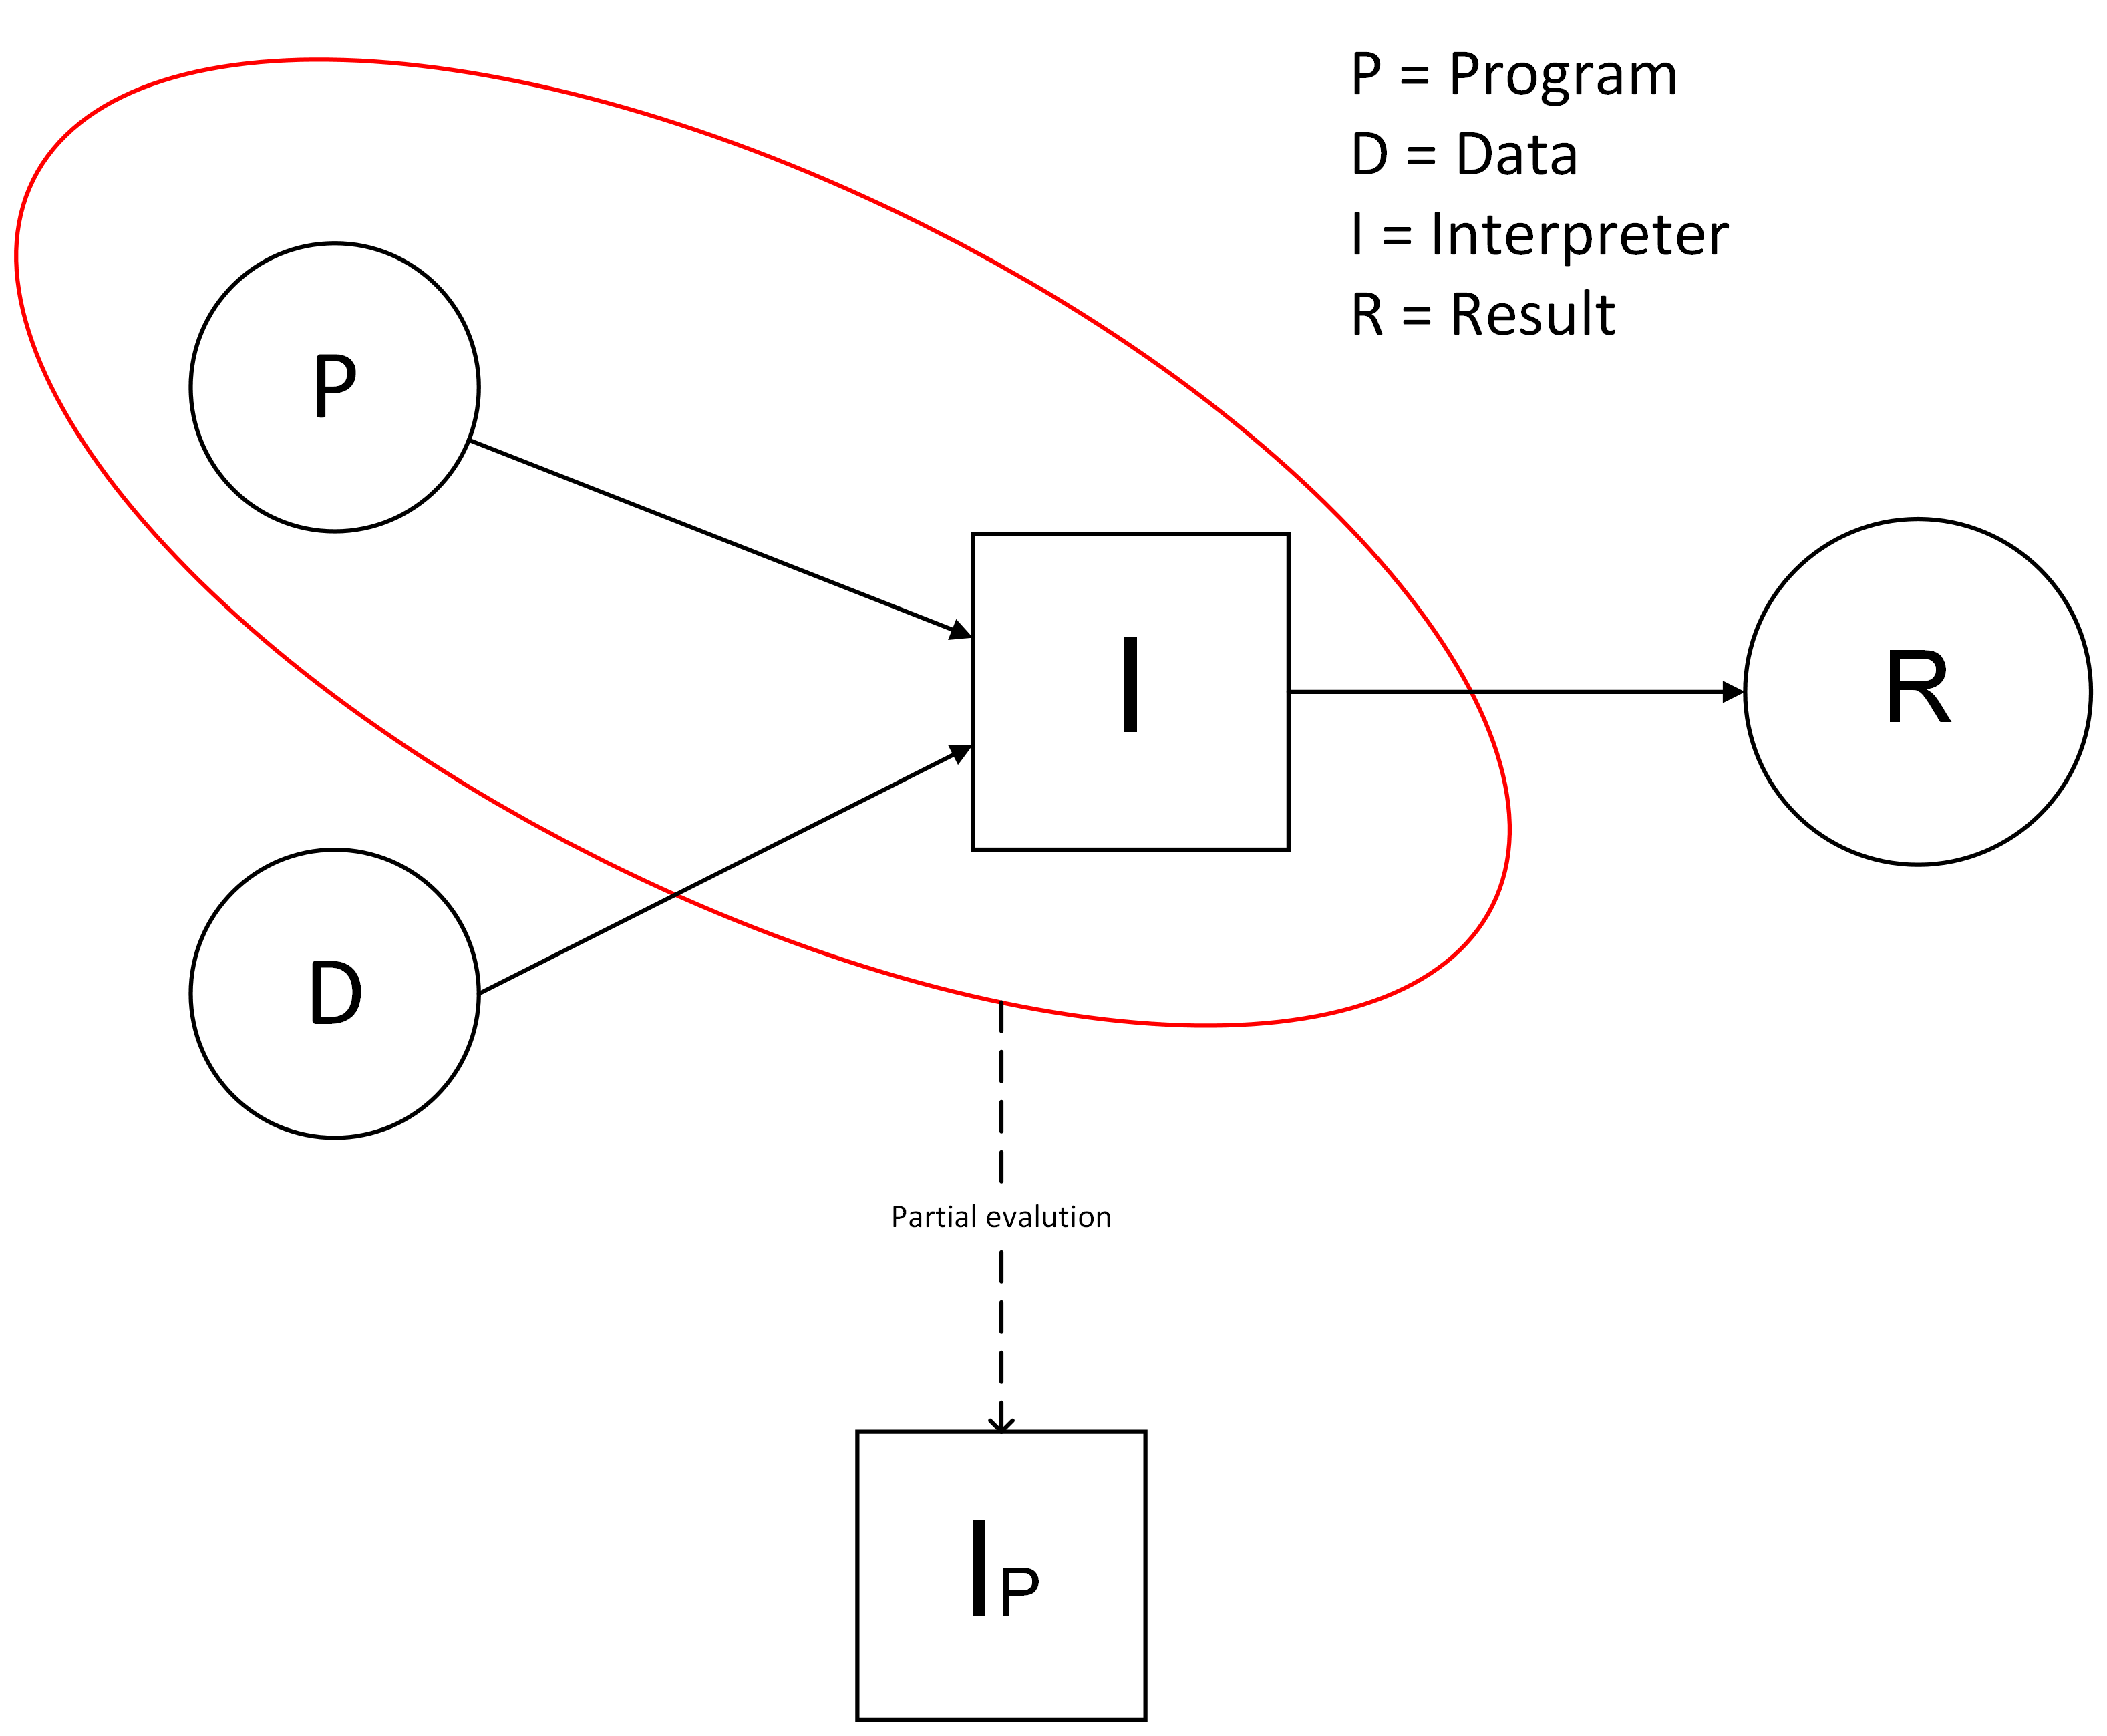
\includegraphics[width=0.8\textwidth]{images/first-futamura-projection.png}
    \caption{První Futamorova projekce}
    \label{fig:futamura-projection}
\end{figure}



\subsubsubsection{Rozdíl mezi meta-tracing a partial evalution}
I~přesto, že obě techniky se snaží dosáhnout stejného cíle, a to vytvořit krátký a efektivní kód, každá z~nich na to jde z~opačného konce. Partial evaluation nejprve nashromáždí co nejvíce dat z~běhu programu, která posléze aplikuje na program a interpret, a tím vytvoří interpret optimalizovaný pro daný program. Klíčové je zde podotknout, že k~tomu, aby tato transformace mohla proběhnout, je nutné, aby daný kód byl několikrát vyhodnocen. Sběr dat z~běhu programu je o~to důležitější při implementaci dynamických jazyků, jelikož množství informací, které lze získat ze statické analýzy těchto jazyků, je minimální. 

Naopak meta-tracing potřebuje pro optimalizaci interpretu pouhé jedno vykonání, během kterého jsou nashromážděny všechny informace o~dané \textit{vykonané cestě} (ang. execution path). To teoreticky znamená, že právě po jednom vykonání má meta-tracing dostatek informací k~optimalizaci této cesty. Jelikož tato optimalizace má výrazný dopad na výkon aplikace, nelze takto optimalizovat každou cestu. Místo toho se meta-tracing snaží vynechat všechny informace, které by tuto cestu činily příliš specifickou. To již bylo možné vidět v~kapitole \ref{meta-tracing-chapter} na obrázku \ref{fig:meta-tracking-example}, kde se do záznamu neuložila kontrola hodnoty argumentu \texttt{x}, ale pouze kontrola, zda je hodnota kladná. Tímto se od sebe jednotlivé techniky nejvíce liší. Zatímco partial evaluation musí vyhodnotit daný blok kódu několikrát k~získání všech potřebných informací, meta-tracing má všechny potřebné informace již po prvním průchodu a využívá heuristik k~vynechaní některých informací, které by činily optimalizaci příliš specifickou. 

Dalším významným rozdílem jsou části kódu, na které se jednotlivé techniky zaměřují. Partial evaluation se zaměřuje na často volané funkce, na které se následně aplikují optimalizace k~vytvoření co největšího kompilačního celku. To znamená, že v~optimalizované funkci dochází k~eliminaci volání vnitřních funkcí (tzn. volání funkce je nahrazeno jejím tělem), k~rozbalování programových smyček nebo k~výpočtu konstantních výrazů. Takto je vytvořen co největší kompilační celek, který je následně přeložen do strojového kódu. Naopak meta-tracing se výhradně zaměřuje na často volané smyčky, jejichž těla jsou obdobně optimalizována a opět přeložena do strojového kódu.   


\newpage


\section{Platforma GraalVM}
GraalVM je virtuální stroj vyvíjený společností Oracle. Jedná se o~modifikaci HotSpotVM, kde serverový C2 překladač byl nahrazen \textit{Graal} překladačem. Nahrazení dynamického překladače je možné díky \textit{Java Virtual Machine Compiler Interface} (JVMCI), což je rozhraní, které je k~dispozici od Java verze 9 a umožňuje integrovat nové dynamické překladače psané v~Javě do JVM. 

Překladač Graal jako vstup přijímá Java bytecode a transformuje ho do interní reprezentace zvané Graal IR (ang. Graal Intermediate Representation). Graal IR je založen na orientované grafové struktuře, která modeluje jak datový tok, tak i~kontrolní tok programu. Zároveň je i v~tzv. \textit{static single assignment form}.\footnote{Static single assignment form je vlastnost interní reprezentace, kde každá proměnná je deklarována před jejím použitím a zároveň je deklarována pouze jednou. Nad interní reprezentací, která splňuje tuto vlastnost je výrazně jednoduší provádět optimalizace. \cite{ssa}} Nad touto datovou strukturou jsou následně prováděny veškeré optimalizace. Jakmile jsou všechny aplikovány, je interní reprezentace přeložena do strojového kódu. Ostatní části GraalVM, jako například správa paměti, jsou pak totožné s~HotspotVM. Architektura GraalVM je znázorněna na~obrázku~\ref{fig:graalvm-architecture}. \cite{graal-ir}


\begin{figure} [h]
    \centering
    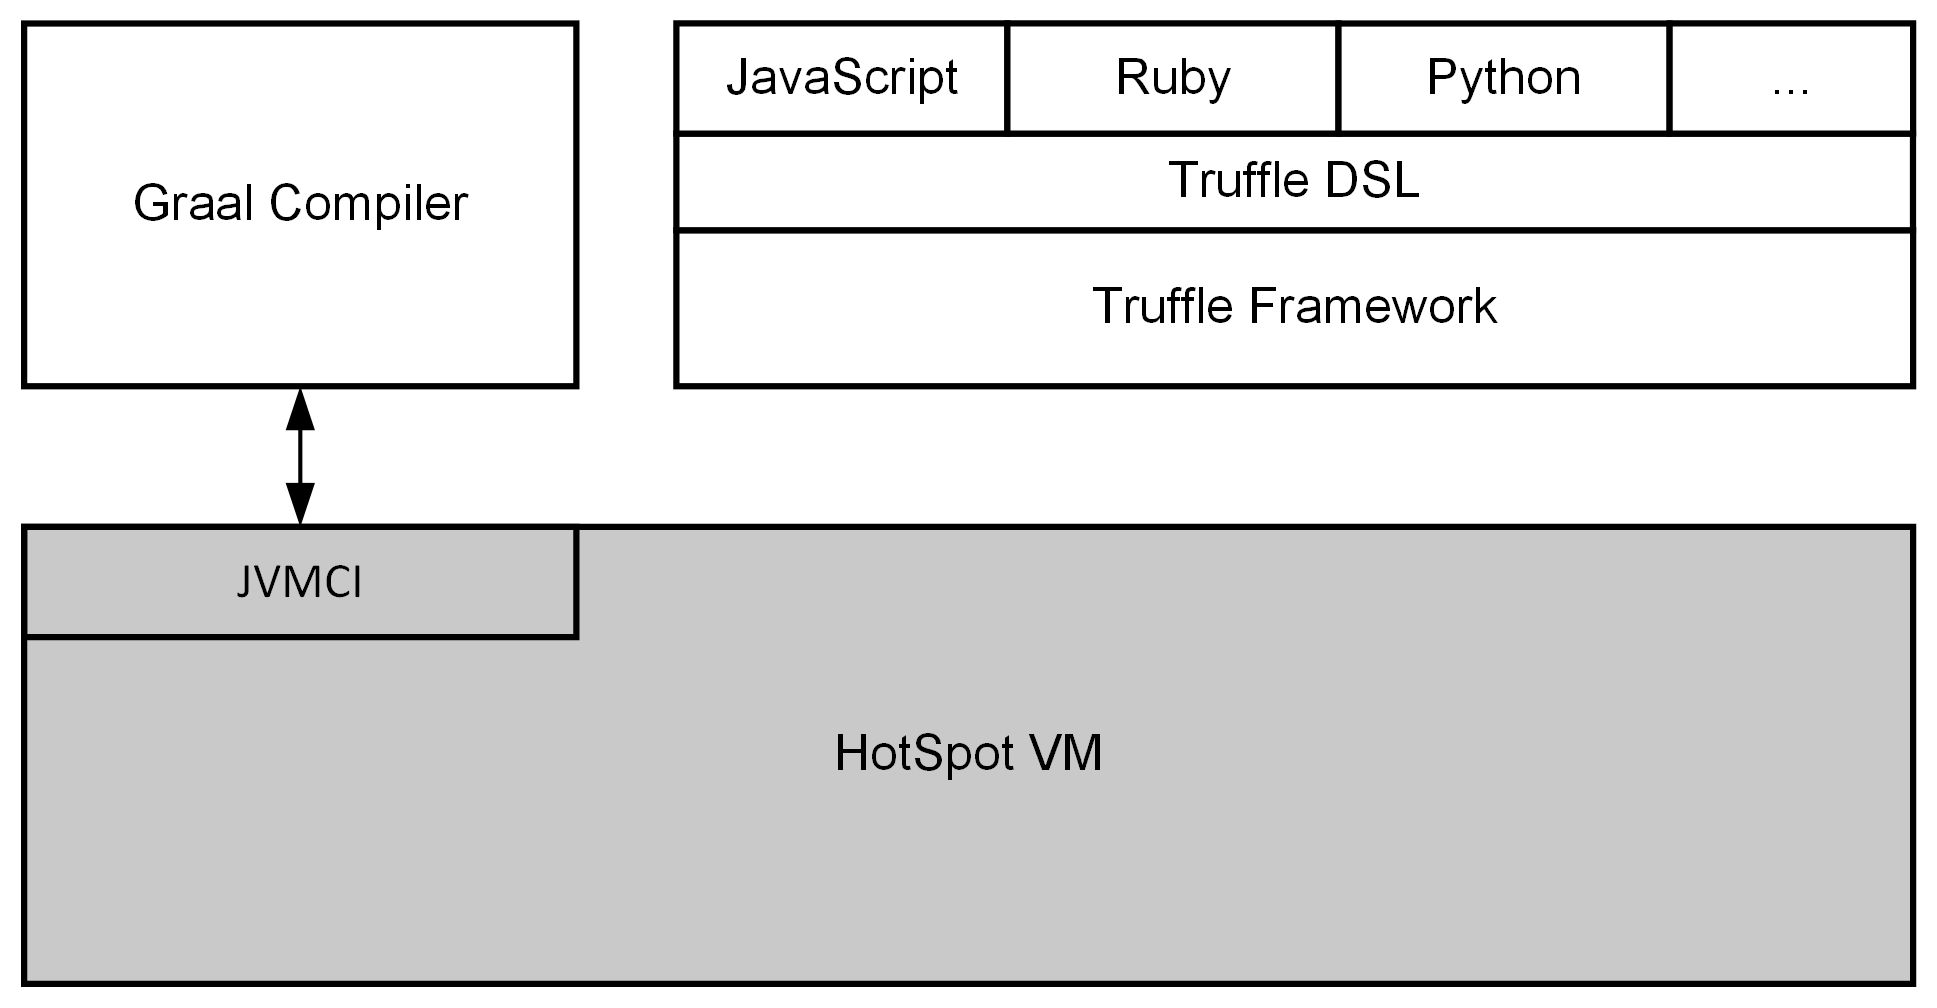
\includegraphics[width= 1\textwidth]{images/graal-architecture.png}
    \caption{Schéma architektury GraalVM}
    \label{fig:graalvm-architecture}
\end{figure}

\subsection{Framework Truffle}
\label{truffle-framework-chapter}
Truffle je framework používaný pro implementaci nových jazyků nad platformou GraalVM. Jedná se o~sadu tříd, rozhraní a anotací, které vývojář při implementaci nového jazyka používá. Rychlost jazyků implementovaných nad GraalVM je pak téměř stejná (nebo lepší) jako v~případě interpretovaných jazyků, kterým byl vytvořen virtuální stroj na míru. Obecně existují dva způsoby, jakými lze implementovat nový jazyk: 

\begin{enumerate}
    \item Napsat interpret, který je relativně jednoduchý na implementaci, ale výrazně pomalejší.
    \item Napsat překladač, který je rychlý, ale mnohonásobně náročnější na implementaci (hlavně při implementaci sofistikovaných optimalizací).
\end{enumerate}

Framework Truffle kombinuje oba výše zmíněné způsoby a bere si z~obou to nejlepší. Programy v jazycích implementovaných ve frameworku Truffle (dále hostované jazyky) jsou reprezentovány jako abstraktní syntaktické stromy (AST), které jsou následně interpretovány. Během této interpretace Truffle sbírá profilující data a~ukládá je do uzlů abstraktního syntaktického stromu. V~případě, že některá z~metod hostovaného jazyka je často volána, Truffle zahájí její JIT překlad. Je~důležité poznamenat, že sám framework Truffle určuje, kdy a jaké části programu budou překládány. Dochází tak ke dvěma rozdílným JIT překladům. První překlad je řízen frameworkem Truffle a druhý je klasický JIT překlad řízený JVM (interpret je stále pouhá Java aplikace).



Hlavním úkolem vývojáře, který se rozhodne implementovat jazyk nad platformou GraalVM, je převést zdrojový kód hostovaného jazyka do abstraktních syntaktických stromů. O~vše ostatní, ať už se jedná o~optimalizace nebo generování strojového kódu, se stará framework Truffle. Tento přístup přináší dvě hlavní výhody:


\begin{enumerate}
    \item Rychlost výzkumných nebo DSL jazyků bude velice podobná rychlosti jejich kompilovaných nebo interpretovaných protějšků (v~případě, že by vůbec vznikly). Úsilí vyložené na implementaci těchto jazyků nad GraalVM by bylo ale výrazně menší.
    \item Budoucí vylepšení překladače Graal nebo frameworku Truffle přinese vylepšení do všech jazyků, které jsou nad platformou implementovány bez jakékoliv změny kódu v~implementaci jazyka. 
\end{enumerate}



\subsection{Sebeoptimalizace AST interpretů}
\label{self-optimalization-of-ast-interpreters}
Při psaní interpretů je běžnou praktikou transformovat zdrojový kód do abstraktního syntaktického stromu (dále AST), který je následně procházen a vyhodnocen. AST interpret vyhodnocuje strom \textit{post-order}, tzn. nejprve jsou vyhodnoceni potomci uzlu a poté uzel samotný. To je intuitivní, jelikož pokud by daný AST strom reprezentoval například funkci sčítání, tak je potomky možné chápat jako argumenty, které musí být vyhodnoceny před vyhodnocením samotného uzlu reprezentujícího sčítání. 

Truffle koncept AST interpretace rozšířil o~tzv. \textit{sebeoptimalizaci}. Sebeoptimalizací je myšleno, že uzel AST stromu se buďto může specializovat na základě vstupních argumentů, a pokrývat tak pouze část původní sémantiky, nebo může nahradit sám sebe za nový uzel, který bude optimalizován na základě profilujících dat. Pokud specializovaný uzel není schopný provést operaci s~aktuálními typy argumentů, dochází k~nové specializaci na základě těchto typů. Tuto opětovnou specializaci lze chápat jako postupné rozšiřování sémantiky. Na začátku specializované uzly pokrývají minimální podmnožinu sémantiky operace a v~případě, že stávající uzel nedokáže provést operaci nad aktuálními operandy, je~uzel znovu specializován, a tím je sémantika operace rozšířena. Tyto uzly musí splňovat následující podmínky:

\begin{enumerate}
    \item \textbf{Úplnost} -- přestože specializovaný uzel pokrývá pouze podmnožinu sémantiky, musí být schopen se znovu specializovat a pokrývat tak zbytek sémantiky operace.  
    \item \textbf{Konečnost} -- po konečném počtu opakovaných specializací musí být uzel v~generickém stavu (pokrývat celou sémantiku operace). To znamená, že tento uzel již nebude nikdy specializován. 
\end{enumerate}


\subsection{Truffle API}
Truffle API je knihovna určená pro vývojáře jazyků k~tvorbě sebeoptimalizujících AST interpretů. Pomocí rozhraní, abstraktních tříd a anotací jsou postupně tvořeny abstraktní syntaktické stromy Truffle, které reprezentují program hostovaného jazyka. Základními prvky knihovny, kterým se bude věnovat tato kapitola, jsou \texttt{Node}, \texttt{RootNode}, \texttt{CallTarget} a \texttt{VirtualFrame}.

\subsubsection{Node}
\texttt{Node} je abstraktní třída, ze které musí dědit všechny uzly abstraktních syntaktických stromů Truffle. Na první pohled může být překvapující, že tato abstraktní třída nemá žádné abstraktní metody, i přesto, že uzly jsou následně vyhodnocovány. Naopak vývojář hostovaného jazyka je zodpovědný za vytvoření těchto metod. Primárním důvodem je fakt, že každý uzel může vracet jiný datový typ, tudíž nelze dopředu definovat dostatečně generickou abstraktní metodu. \texttt{Node} obsahuje spoustu pomocných funkcí, které slouží k~modifikaci abstraktního syntaktického stromu Truffle. Například metody jako \texttt{insert} nebo \texttt{replace} slouží k~vložení či nahrazení potomka. V~kapitole \ref{chapter-macros-implementation} je pak možné se dočíst, jak je metoda \texttt{replace} použita k~expanzi maker. 

Každá třída, která není abstraktní a dědí z~\texttt{Node} musí definovat metodu, jejíž jméno musí začínat prefixem \texttt{execute}. Potomka tohoto uzlu je pak možné definovat pomocí anotace \texttt{@Child}. V~případě, že potomků je více, existuje anotace \texttt{@Children}, která slouží k~definování pole potomků. Potomci nemohou být označeni klíčovým slovem \texttt{final}, jelikož může dojít k~nahrazení potomka specializovanějším (např. pomoci výše zmíněné metody \texttt{replace}). Důležité je zmínit, že všechny vlastnosti třídy s~anotací \texttt{@Child} jsou překladačem Graal vnímány jako konstanty. Vlastnosti označené \texttt{@Children} mají dokonce silnější sémantiku než \texttt{final}, a to takovou, že nejen pole samotné je vnímáno jako konstanta, ale i jeho prvky jsou překladačem Graal vnímané jako konstanty.  

Pro úplnost je vhodné zmínit anotaci \texttt{@CompilationFinal}. Jak je možné odvodit z~názvu, jedná se o~anotaci, která má stejnou sémantiku jako klíčové slovo \texttt{final}. Vlastnosti, které neobsahují anotaci \texttt{@Child}, ale stejně je důležité, aby byly překladačem Graal vnímané jako konstantní, obsahují právě tuto anotaci. Anotace dokonce obsahuje vlastnost \texttt{dimensions}, která se používá na vlastnosti typu pole. Definuje, zda i prvky pole mají být vnímány jako konstanty. Ve skutečnosti anotace \texttt{@Child} sémanticky odpovídá anotaci \texttt{@CompilationFinal} a anotace \texttt{@Children} sémanticky odpovídá anotaci \texttt{@CompilationFinal(dimensions = 1)}. 

Ve zdrojovém kódu \ref{additional-node-impl} je pak možné vidět jednoduchou implementaci uzlu pro sčítání. Uzel dědí z~abstraktní třídy \texttt{SchemeNode}, která obsahuje onu abstraktní metodu \texttt{executeInt}. Uzel obsahuje dva potomky \texttt{leftNode} a \texttt{rightNode}. V~těle metody jsou pak prvky prvně vyhodnoceny a následně sečteny. Metoda obsahuje pouze jeden argument typu \texttt{VirtualFrame}, kterému je věnována následující kapitola.


\begin{listing} [H]
    \begin{minted}{java}
        public final class AdditionNode extends SchemeNode {
            @SuppressWarnings("FieldMayBeFinal")
            @Child
            private SchemeNode leftNode, rightNode;
        
            public AdditionNode(SchemeNode leftNode, SchemeNode rightNode) {
                this.leftNode = leftNode;
                this.rightNode = rightNode;
            }
        
            @Override
            public int executeInt(VirtualFrame frame) {
                int leftValue = this.leftNode.executeInt(frame);
                int rightValue = this.rightNode.executeInt(frame);
                return leftValue + rightValue;
            }
        }
    \end{minted}
    \caption{Příklad implementace uzlu pro sčítání argumentů typu \texttt{int}}
    \label{additional-node-impl}
\end{listing}


\subsubsection{VirtualFrame}
\label{chapter-virtualFrame}
\texttt{VirtualFrame} je třída odpovídající klasickému zásobníkovému rámci. Jedná se o~datovou strukturu, která slouží k~ukládání potřebných dat spojených s~voláním funkce. Jedná se o~data jako například lokální proměnné funkce nebo její parametry. \texttt{VirtualFrame} je vytvořen automaticky při zavolání funkce a je vytvořen na základě třídy  \texttt{FrameDescriptor}. Tato třída může být chápána jako „popisovač“, podle kterého jsou následně vytvořeny instance třídy \texttt{Virtual\-Frame}. Obsahuje informace jako například počet lokálních proměnných a jejich typ, které jsou následně využity k~vytvoření paměťově optimální instance. Lokální proměnné primitivního typu (např. \texttt{int}, \texttt{double}, \texttt{float}) jsou uloženy v~poli typu \texttt{long[]}, zatímco všechny ostatní proměnné jsou uloženy v~poli typu \texttt{Object[]}. Stojí za povšimnutí, že všechny primitivní typy je možné převést na hodnoty typu \texttt{long}. Například hodnoty typu \texttt{double} lze převést na hodnoty typu \texttt{long} pomocí statických metod \texttt{Double.doubleToRawLongBits()} a \texttt{Double.longToDoubleBits}. \cite{truffle-clojure}



\subsubsection{RootNode}
\texttt{RootNode} je speciálním uzlem (potomkem třídy \texttt{Node}), který reprezentuje kořen daného stromu. Jedná se opět o~abstraktní třídu stejně jako \texttt{Node}. Na rozdíl od \texttt{Node} obsahuje již abstraktní metodu \texttt{execute}, kterou je nutné implementovat. To znamená, že \texttt{RootNode} slouží k~zapouzdření jednoho nebo více uzlů, které je možné následně vyhodnotit. To nejčastěji reprezentuje části hostovaného jazyka, které lze volat. Může se jednat nejen o~procedury či funkce, ale i o~vstupní body programu (například v~Javě se jedná o~statickou metodu \texttt{main}). V~praxi se ale přímo \texttt{RootNode} k~volání funkcí nepoužívá. Používá se \texttt{CallTarget}, který je popsán v~následující kapitole. 


\subsubsection{CallTarget}
\label{chapter-callTarget}
\texttt{CallTarget} je poslední abstrakcí nad \texttt{RootNode}, avšak již se nejedná o~abstraktní třídu, ze které by měl vývojář dědit. Místo toho se jedná o~rozhraní obsahující metodu \texttt{call}, která přijímá libovolný počet argumentů a slouží k~vyhodnocení uzlů uložených v~\texttt{RootNode}. Implementace tohoto rozhraní je pak poskytována aktuálním běhovým prostředím (např. GraalVM Community Edition nebo GraalVM Enterprise Edition). Hlavním cílem této abstrakce je:

\begin{enumerate}
    \item Sbírat a ukládat profilující informace z~běhu aplikace. Nejčastěji se jedná o~informace jako počet volání dané metody k~určení, zda je vhodným kandidátem pro JIT kompilaci. 
    \item Vytvořit novou instanci třídy \texttt{VirtualFrame}, která bude obsahovat potřebné argumenty k~uskutečnění daného volání. 
\end{enumerate}

    


\subsection{Specializace}
\label{specialization-chapter}
Specializace jsou jednou z~klíčových optimalizací frameworku Truffle. V~této kapitole je popsán princip specializací spolu s~partial evaluation, která je nezbytnou součástí tvorby velice efektivního strojového kódu. Kapitola vychází ze zdroje~\cite{truffle-dsl-thesis}.

Jak již bylo nastíněno v~předchozí kapitole, specializace je možné vnímat jako dělení sémantiky operace na více částí (specializací). Hlavními výhodami tohoto dělení je například: 

\begin{itemize}
    \item Rozdělení komplexních operací na menší části. To je obecně dobrou praktikou v~softwarovém inženýrství. Tyto menší části lze pak jednodušeji implementovat a testovat. 
    \item Malé specializované metody umožní generovat velice rychlý a kompaktní strojový kód.
\end{itemize}

Obecná implementace specializací se skládá ze dvou částí. Tou první je kontrola, zda aktuální specializace pokrývá sémantiku na základě typu vstupních argumentů. Druhou částí je pak samotné provedení logiky operace. Jinými slovy, logika operace je chráněna (ang. \textit{guarded}) typovou kontrolou vstupních argumentů. Pokud typová kontrola vstupních argumentů není úspěšná (specializace nepokrývá sémantiku danou typem vstupních argumentů), může dojít ke dvěma případům:

\begin{enumerate}
    \item V~případě, že se daný uzel pouze interpretuje, tzn. uzel nebyl přeložen do strojového kódu, dojde pouze ke změně jeho vnitřního stavu. Tato změna reprezentuje přidání nové specializace, která pokrývá sémantiku danou vstupními argumenty. 
    \item V~případě, že uzel již byl přeložen do strojové kódu, dochází k~deoptimalizaci a strojový kód je zahozen. Uzel se opět začne interpretovat a změní se jeho vnitřní stav, stejně jako v~předchozím případě. Jakmile Truffle vyhodnotí, že je uzel opět vhodným kandidátem k~JIT kompilaci, dojde opět k~překladu do strojového kódu. Takto nově vytvořený strojový kód je rozšířen o~sémantiku, která způsobila předchozí deoptimalizaci.
\end{enumerate}


Pokud uzel reprezentuje operaci sčítání, ve většině dynamických jazyků lze vytvořit tři specializace \texttt{I}, \texttt{D} a \texttt{S}. Specializace \texttt{I} reprezentuje sčítání čísel typu \texttt{integer}, specilizace \texttt{D} sčítání čísel typu \texttt{double} a specializace \texttt{S} reprezentuje konkatenaci řetězců. Všechny specializace dohromady pokrývají celou sémantiku operátoru sčítání. Na obrázku \ref{fig:node-transitions} je takový uzel zobrazen se všemi stavy, do kterých se může dostat.  

\begin{figure}
    \centering
    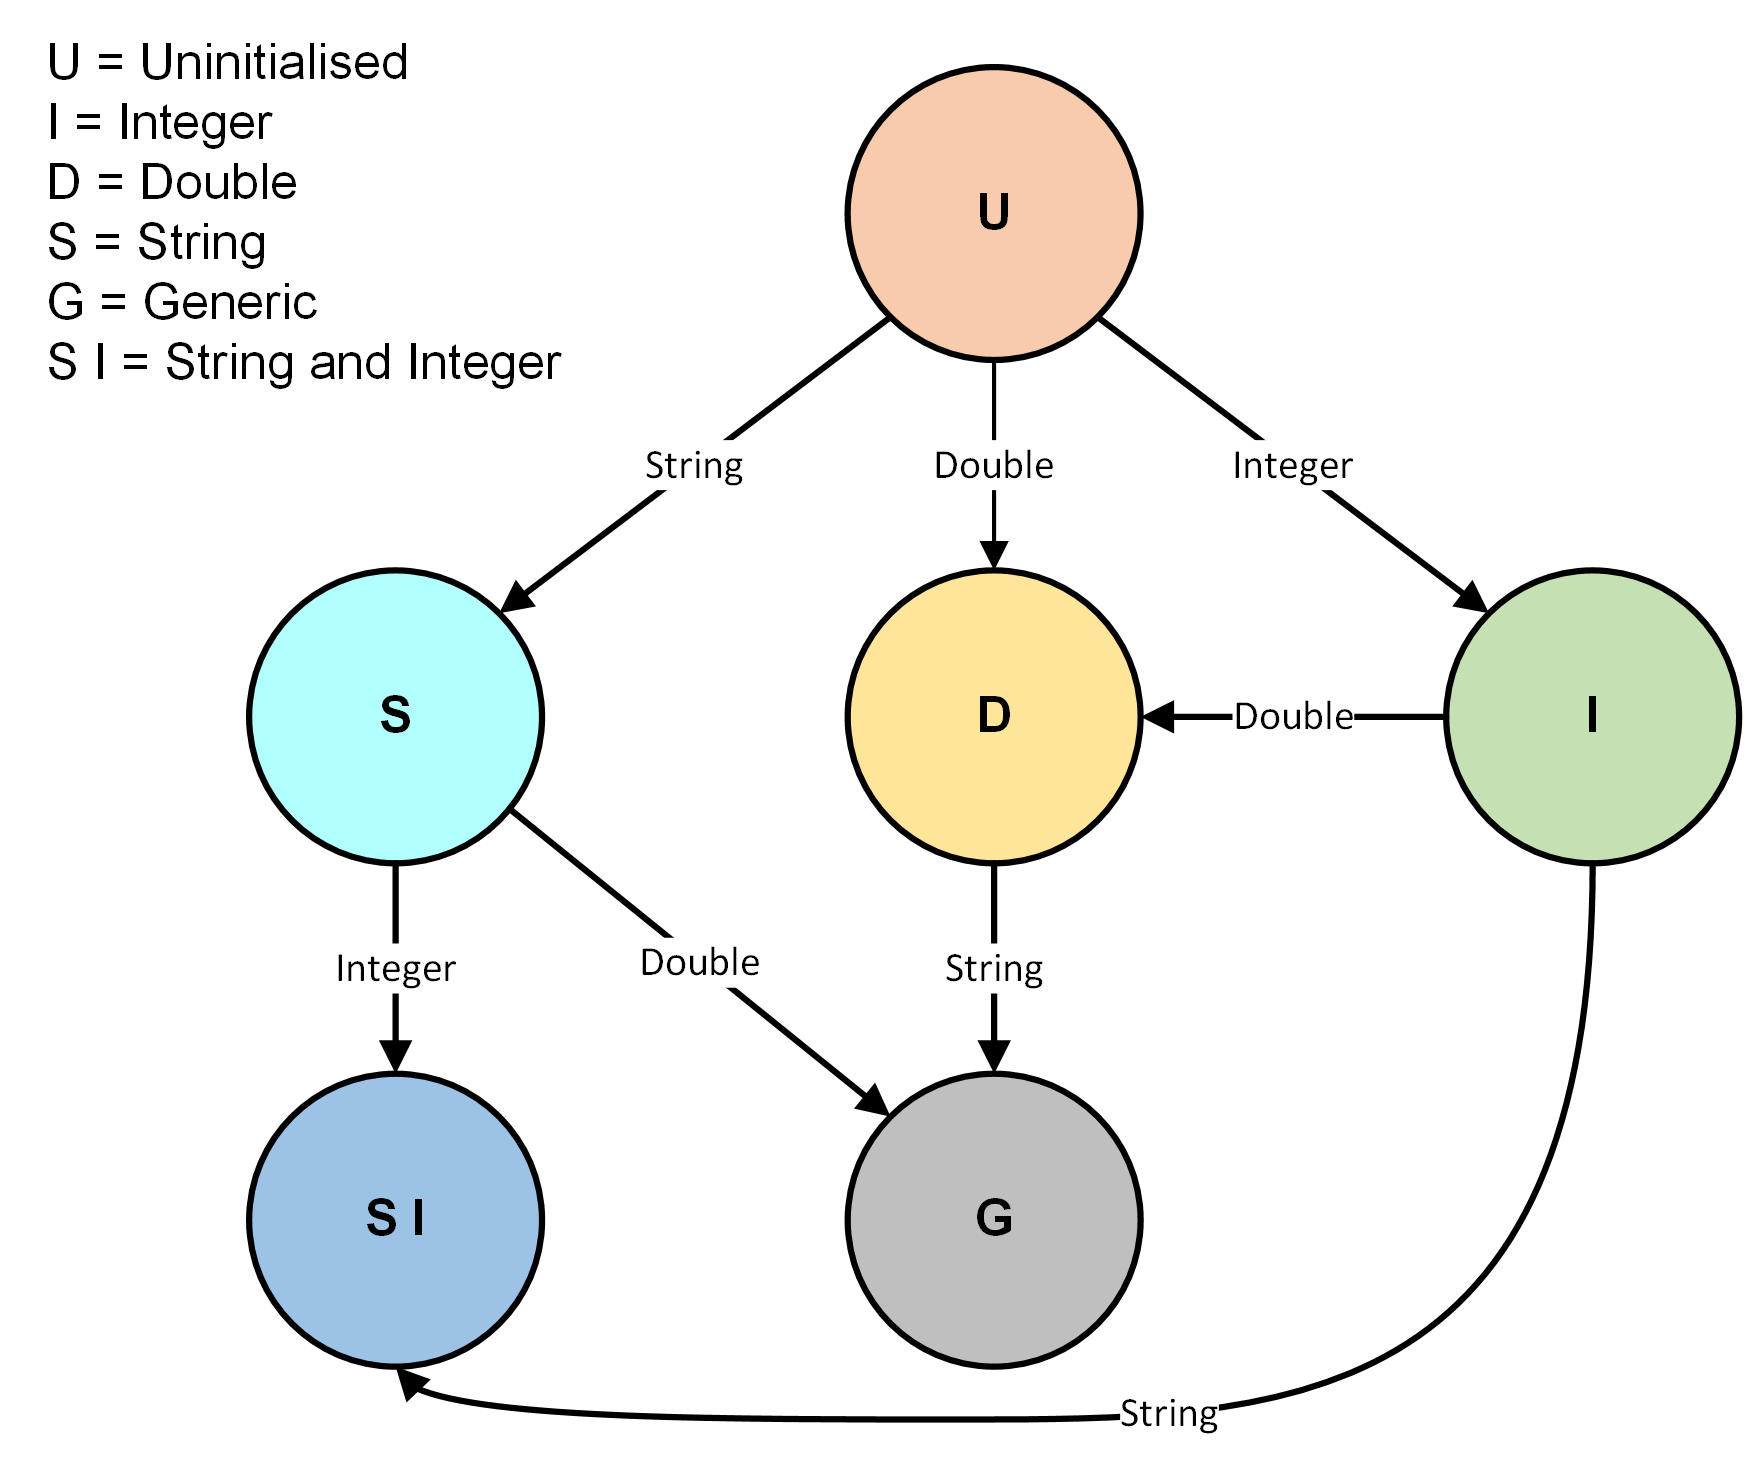
\includegraphics[width= 0.6\textwidth]{images/node-transitions.png}
    \caption{Uzel reprezentující operaci sčítání se všemi možnými přechody od neinicializovaného stavu \texttt{U} až do generického stavu \texttt{G}}
    \label{fig:node-transitions}
\end{figure}

Na začátku je uzel v~\textit{neinicializovaném} stavu. Po prvním zavolání se uzel specializuje na základě typu vstupních argumentů a přejde do stavu \texttt{I}, \texttt{D} nebo \texttt{S}. Pokud by specializace dokázala obsloužit všechny budoucí volání (to by znamenalo, že operátor sčítání byl volán pouze s~jedním typem argumentů) nazýváme takový uzel \textit{monomorfní}. Takový uzel je co se týče výkonu optimální, ale není možné garantovat, že v~budoucnu tento předpoklad nebude porušen.

V~případě, že tento předpoklad je porušen, nelze jen jednoduše přejít do jiné specializace a znovu se specializovat jen na základě nových vstupních argumentů, protože by bylo možné dojít do stavu, kdy se alternuje mezi dvěma nebo více stavy, což porušuje podmínku konečnosti. Nutné je zmínit, že deoptimalizace má výrazný vliv na výkon aplikace, tudíž alternací mezi několika stavy by výkon výrazně klesl. Je potřeba, aby uzel byl schopný pokrýt více specializací zároveň, jinými slovy, pokrýt více typů vstupních argumentů. Takový uzel nazýváme \textit{polymorfní}. Implementovat všechny možné kombinace jednotlivých specializací je nepředstavitelné, protože počet kombinací roste exponenciálně vzhledem k~počtu specializací. Proto Truffle využívá \textit{zřetězení} (ang. chaining), kde specializace jsou řetězeny za sebou a první specializace, která je schopná pokrýt sémantiku danou vstupními argumenty je použita. Je zřejmé, že s~rostoucím počtem specializací klesá výkon aplikace. Uzel, který obsahuje všechny specializace, je označován jako generický. 

Pokud ve výše zmíněné operaci sčítání je funkce nejprve volána s~argumenty typu \texttt{double}, přejde uzel do specializace \texttt{D}. Poté bude funkce zavolána s~argumenty typu \texttt{string}. V~takovém případě, jak je možné vidět na obrázku \ref{fig:node-transitions}, nedojde k~přechodu do specializace \texttt{S}, ale do generické specializace \texttt{G}. Uzel se tak stal polymorfním, a to zřetězením specializace \texttt{D} a \texttt{S}. Pokud by v~tomto případě nebyla zvolena specializace \texttt{G}, ale specializace \texttt{S} mohlo by dojít k~výše zmíněným alternacím a byla by porušena podmínka konečnosti. 


Dále je možné vidět na obrázku \ref{fig:node-transitions}, že nikdy nedojde k~zřetězení specializace \texttt{D} se specializací \texttt{I}, a to z~důvodu, že specializace \texttt{I} je striktní podmnožinou specializace \texttt{D} (celá čísla jsou podmnožinou racionálních čísel). Nemusí tak vždy dojít k~řetězení jednotlivých specializací, ale specializace může být zcela nahrazena jinou specializací, která zároveň pokrývá sémantiku předchozí specializace. Všechny možnosti, jak lze jednotlivé specializace kombinovat jsou popsány v~kapitole \ref{specializations-and-performance}. 


Specializace jsou reprezentovány v~uzlu jako stavy, do kterých na základě typu vstupních argumentů uzel může přejít. V~podstatě se jedná o~konečný deterministický automat, který vždy začíná v~neinicializovaném stavu. Po prvním přechodu vždy přejde do monomorfního stavu, který je co se týče výkonu optimální. Další řetězení specializací činí uzel polymorfní. Pokud má uzel aktivní všechny specializace, je v~generickém stavu a nedojde tak již k~žádné další specializaci. Generický stav uzlu je samozřejmě z~hlediska výkonu nejhorší. 


\subsubsection{Specializace a výkon aplikace}
\label{specializations-and-performance}
Výkonné implementace virtuálních strojů jsou založeny na velice agresivních optimalizacích. Nejčastěji jsou tyto optimalizace založeny na dvou předpokladech: 

\begin{enumerate}
    \item \textit{Hodnota se nezmění.} Na základě tohoto předpokladu jsou proměnné vnímány běhovým prostředím jako konstanty. Použití těchto proměnných lze následně optimalizovat pomocí výpočtu konstantních výrazů a jejich propagace. To nejčastěji vede k odstranění větvení, a tím se otevírá prostor pro další optimalizace.
    \item \textit{Typ se nezmění.} Na tomto předpokladu jsou většinou založeny specializace Truffle. Tímto je výrazně redukována velikost generovaného strojového kódu, jelikož je možné odstranit větvení vybírající správnou logiku dle typu vstupních argumentů. Tento typ spekulace je obzvláště důležitý pro dynamické jazyky. 
\end{enumerate}

\begin{figure} [h]
    \centering
    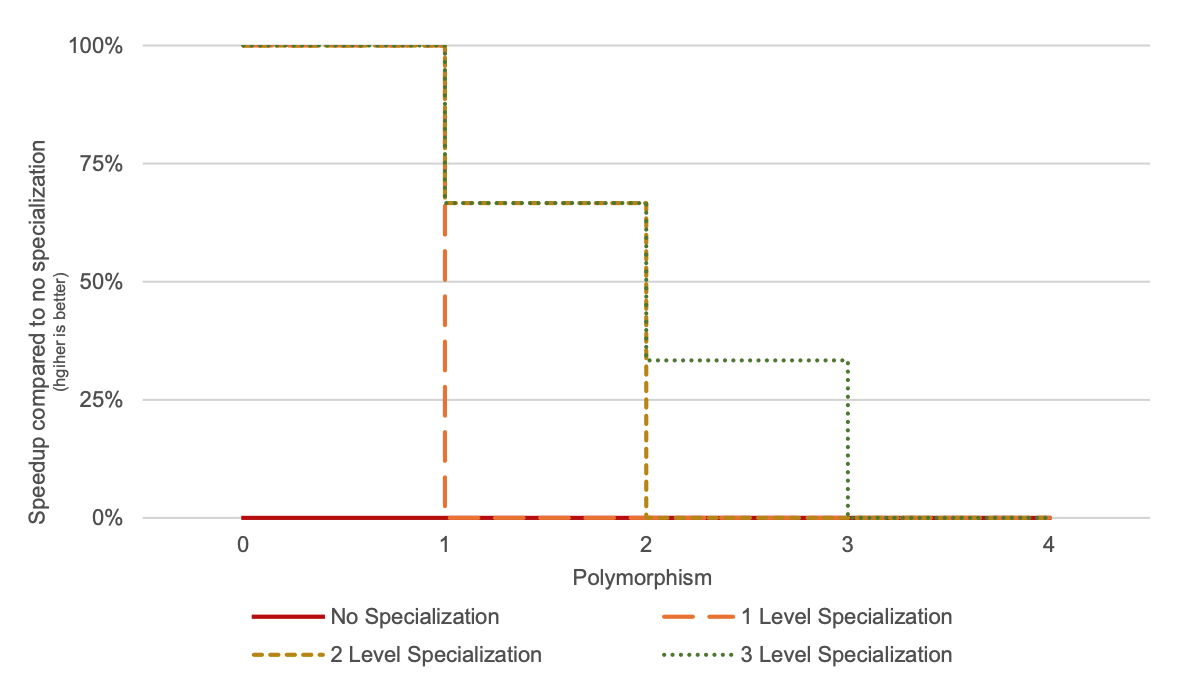
\includegraphics[width= 1\textwidth]{images/perf-cliff.png}
    \caption{Porovnání rychlosti s~rostoucím počtem specializací. V~případě, že počet specializací je nízký, může dojít k~náhlému propadu ve výkonu a způsobit tzv. performance cliff \cite{truffle-dsl-thesis}}
    \label{fig:performance-cliff}
\end{figure}

V~předchozí kapitole již bylo zmíněno, že součástí specializací jsou kontroly (ang. \textit{guards}), které zaručí správný výběr logiky na základě typu vstupních argumentů. V~případě, že kontroly specializací selžou, je nutné ke stávající specializaci zřetězit novou specializaci a rozšířit tak sémantiku operace. V~nejhorším případě se uzel může dostat do generického stavu, který je nejtěžší na optimalizaci. Přechodem do generického stavu může být způsoben náhlý propad ve výkonu, který je často nazýván \textit{performance cliff}.




Náhlé změně výkonu lze předejít několika vrstvami specializací. Cílem je předejít přechodu do generického stavu, který je z hlediska výkonu nejhorší. Obrázek~\ref{fig:performance-cliff} ukazuje možný propad výkonu s~rostoucím stupněm polymorfismu. Stupeň polymorfismu vyjadřuje, s~kolika různými typy vstupních argumentů byla operace již zavolána. Pokud například byla operace sčítání prvně zavolána se vstupními argumenty typu \texttt{double} a poté s~argumenty typu \texttt{string}, je stupeň polymorfismu roven dvěma. Je důležité poznamenat, že nelze určit dle stupně polymorfismu, zda je uzel v~generickém stavu, či ne. V~příkladu, který je zobrazen na obrázku \ref{fig:node-transitions} je vidět, že stav \texttt{SI} má stejný stupeň polymorfismu jako generický stav \textit{G}. Stav \texttt{SI} je užitečný jen za předpokladu, že je efektivnější než stav \texttt{G}. Vrstvením jednotlivých specializací lze předejít náhlým výkonnostním změnám. Existují tři možnosti~\cite{truffle-dsl-thesis}, jakými lze specializace vrstvit (viz obrázek~\ref{fig:chaining-replacement-adoption}).


\begin{itemize}
    \item \textbf{Řetězení} (ang. chaining) sloučí dvě specializace tak, že se nejprve vykonají kontroly první specializace a v~případě že selžou, zavolají se kontroly druhé specializace. Je doporučeno, aby množiny vstupních argumentů jednotlivých specializací byly disjunktní. Řetězení je obecná technika, kterou využívá například i \textit{polymorphic inline caches}.
    \item \textbf{Nahrazení} (ang. replacement) sloučí dvě specializace tak, že první specializace je nahrazena druhou specializací. To je možné jen v~případě, že vstupní argumentu první specializace jsou podmnožinou vstupních argumentů druhé specializace. 
    \item \textbf{Adopce} (ang. adoption) sloučí dvě specializace tak, že druhá specializace se stane potomkem první specializace. V~praxi se adopce používá například k~rozdělení komplexních operací na menší části. Například jazyk R nemá skalární hodnoty samotné, ale má vektor skalárních hodnot. Je možné vytvořit uzly se specializacemi pro aritmetiku se skalárními hodnotami, které budou potomky uzlů se specializacemi pro práci se samotnými vektory.  
\end{itemize}



\begin{figure}
    \centering
    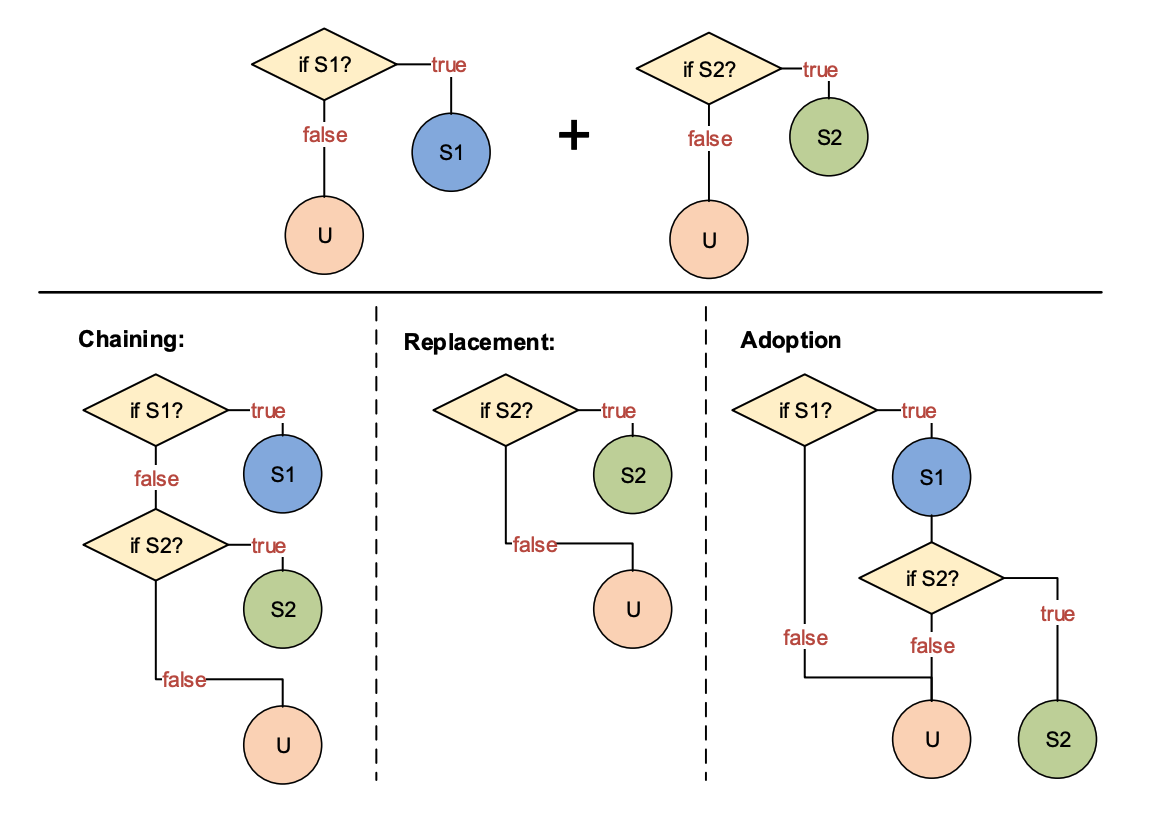
\includegraphics[width= 1\textwidth]{images/combining-techniques2.png}
    \caption{Varianty vrstvení dvou specializací k~zamezení náhlému propadu ve výkonu (performance cliff) \cite{truffle-dsl-thesis}}
    \label{fig:chaining-replacement-adoption}
\end{figure}

Při psaní interpretu je pak potřeba najít rovnováhu v~počtu specializací pro každou operaci. V~případě, že specializací je málo, uzel se brzy dostane do generického stavu a vzniká tak výše zmíněný náhlý propad ve výkonu. Pokud naopak bude specializací příliš mnoho, časté deoptimalizace a překlady do strojového kódu se také negativně projeví na rychlosti interpretovaného jazyka.

\newpage


\subsubsection{Specializace a partial evaluation}
Partial evaluation (dále PE) na platformě GraalVM je ve své podstatě velice agresivní aplikace optimalizací, jako například rozbalování programových smyček, eliminace volání metod nebo výpočet konstantních výrazů na interpret a~program samotný (včetně dat z~běhu programu). Důležité je zmínit, že vývojář interpretu si je vědom, že na daný kód může být aplikována PE, a tudíž píše kód interpretu tak, aby na něj mohla být PE aplikována jednoduše (píše tzv. \textit{PE-friendly code}). Na obrázku~\ref{fig:pe-example-1} lze například vidět, že použitím anotace \texttt{@CompilationFinal} dochází k~eliminaci větvení a vzniká tak krátký a efektivní strojový kód. 

\begin{figure} [h]
    \centering
    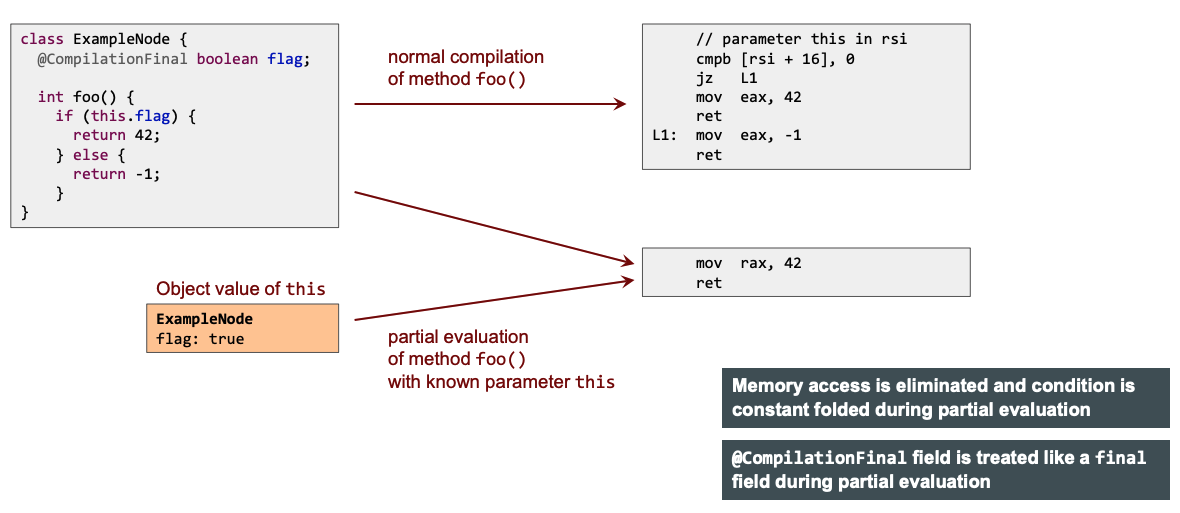
\includegraphics[width= 1\textwidth]{images/pe-exampke-1.png}
    \caption{Použití anotace \texttt{@CompilationFinal} u vlastnosti způsobí eliminaci větvení, a~tudíž výsledný strojový kód je výrazně kratší a~efektivnější \cite{truffle-pe-presentation}}
    \label{fig:pe-example-1}
\end{figure}

Na obrázku \ref{fig:pe-example-2} je další ukázka toho, jak PE dokáže zefektivnit a zjednodušit kód. V~tomto případě se jedná již o~program, ve kterém dochází ke sečtení tří hodnot. Nejprve je vytvořen abstraktní syntaktický strom Truffle, který daný program reprezentuje. I~přesto, že interpret pracuje nad třídami jako jsou \texttt{Add} nebo \texttt{Arg},\footnote{Jedná se o~potomky třídy \texttt{Node}, tudíž všechny obsahují metodu \texttt{execute} a potomci jsou deklarováni pomocí anotace \texttt{@Child} nebo \texttt{@Children}.} Překladač Graal má stále přistup k~bytecode jednotlivých tříd skrze reflexi. Bytecode je nejprve převeden do Graal IR a následně je aplikována PE. Jak je možné vidět, postupnou aplikací optimalizací (v~tom případě výpočet konstantních výrazů a eliminace volání metod) dochází k~postupnému vkládání těl jednotlivých \texttt{execute} metod. Díky těmto optimalizacím nejprve dochází k~odstranění tříd \texttt{Add} a \texttt{Arg} a následně dochází i k~eliminaci všech jejich \texttt{execute} metod. Výsledkem je krátký a velice efektivní kód, ve kterém byly eliminovány jakékoliv známky interpretu. Nutno zmínit, že všechny tyto transformace probíhají nad Graal IR, tudíž jednotlivé transformace kódu viditelné na obrázku \ref{fig:pe-example-2} slouží pouze k~demonstračním účelům.  

\newpage

\begin{figure} [h]
    \centering
    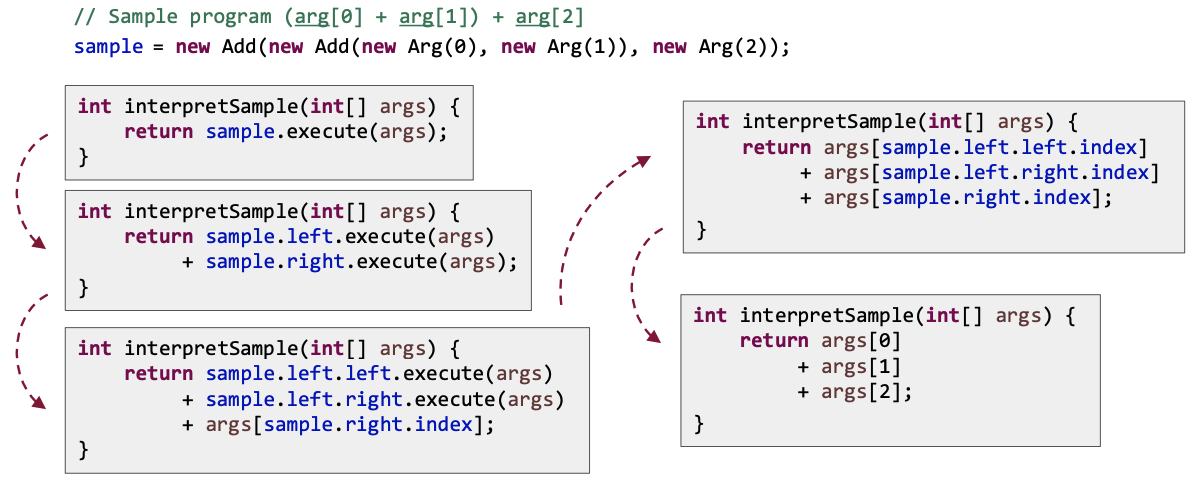
\includegraphics[width= 1\textwidth]{images/pe-example-2.png}
    \caption{Aplikace PE na program reprezentující sčítání tří hodnot. Postupně jsou eliminovány jakékoliv známky interpretu \cite{truffle-pe-presentation}}
    \label{fig:pe-example-2}
\end{figure}

Jak již bylo popsáno v~kapitole \ref{truffle-framework-chapter}, Truffle si řídí JIT kompilaci metod interpretovaného jazyka. Aby metoda byla vhodným kandidátem pro JIT kompilaci, musí splňovat následující podmínky:

\begin{itemize}
    \item Počet volání dané metody musí překročit hranici pro JIT kompilaci.
    \item Abstraktní syntaktický strom Truffle, který reprezentuje danou metodu, musí být stabilní. Strom je stabilní ve chvíli, kdy nedochází k~dalším specializacím.  
\end{itemize}

Jakmile metoda splňuje obě podmínky, dochází k~JIT kompilaci řízené frameworkem Truffle, jejíž první fází je PE. Touto fází se liší od tradiční JVM řízené JIT kompilace. To znamená, že překladač Graal je rozšířen o~tuto fázi vzhledem k~C2 překladači a aplikuje ji pouze v případě, že je kompilace řízena frameworkem Truffle. Abstraktní syntaktický strom Truffle, reprezentující kompilovanou metodu, je nejprve převeden do interní reprezentace (Graal IR), na kterou je následně aplikována PE. Výsledkem je efektivnější Graal IR, který již prochází standardními fázemi běžné JIT kompilace. Celý proces je vizualizován na obrázku \ref{fig:tree-specialization-PE}.


\begin{figure} [h]
    \centering
    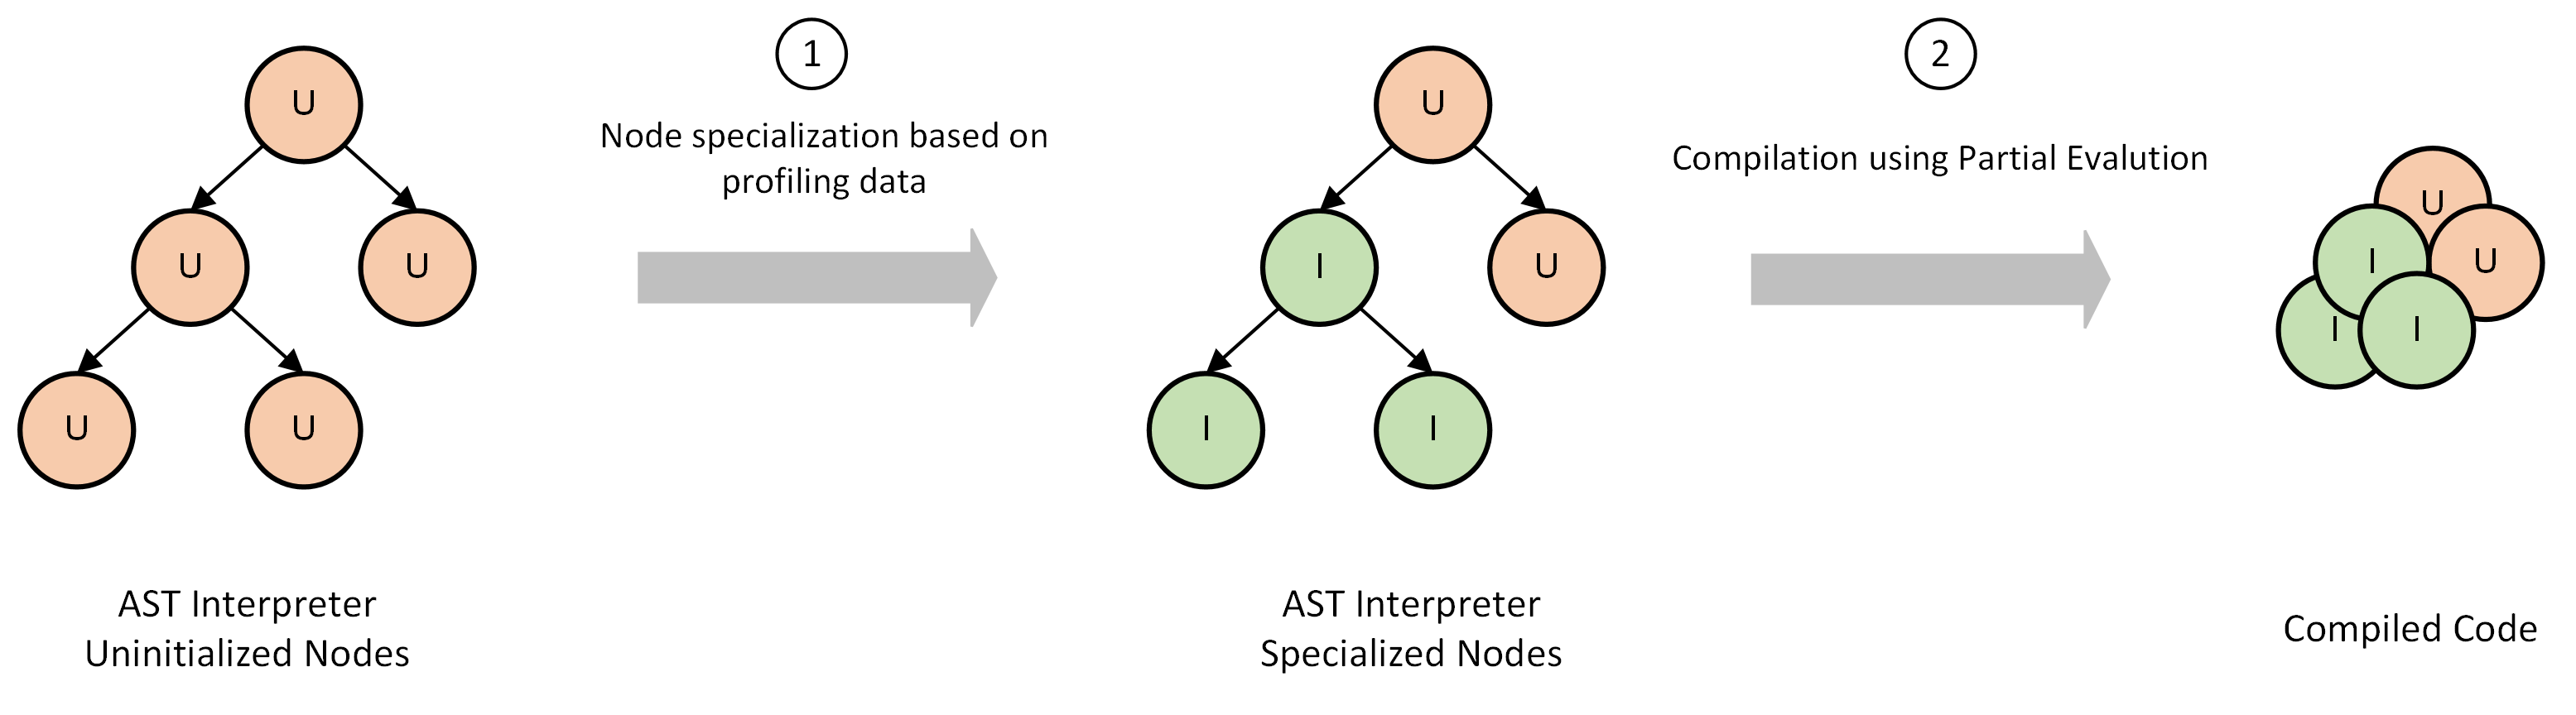
\includegraphics[width= 1\textwidth]{images/nodes-partial-evaluation.png}
    \caption{Na základě profilujících dat se uzly specializují {\Large \textcircled{\normalsize 1}}. Jakmile je strom stabilní a~počet volání metody překročí hranici pro JIT kompilaci, je na specializovaný strom nejprve aplikována PE a~poté je přeložen do strojového kódu~{\Large \textcircled{\normalsize 2}}~\cite{one-vm-to-rule-them-all}}
    \label{fig:tree-specialization-PE}
\end{figure}



V~případě, že předpoklad stability stromu je porušen a strojový kód nedokáže pokrýt sémantiku vstupních argumentů, dochází k~deoptimalizaci. Tímto dojde k~odstranění dříve přeloženého strojového kódu a přechází se k~interpretaci. Abstraktní syntaktický strom Truffle je znovu specializován na základě nových vstupních argumentů a v~případě, že jsou splněny obě výše zmíněné podmínky, je zahájena nová JIT kompilace, která je opět řízena frameworkem Truffle. Proces deoptimalizace je vizualizován na obrázku \ref{fig:tree-deopt-and-respecilized}.


\begin{figure} [h]
    \centering
    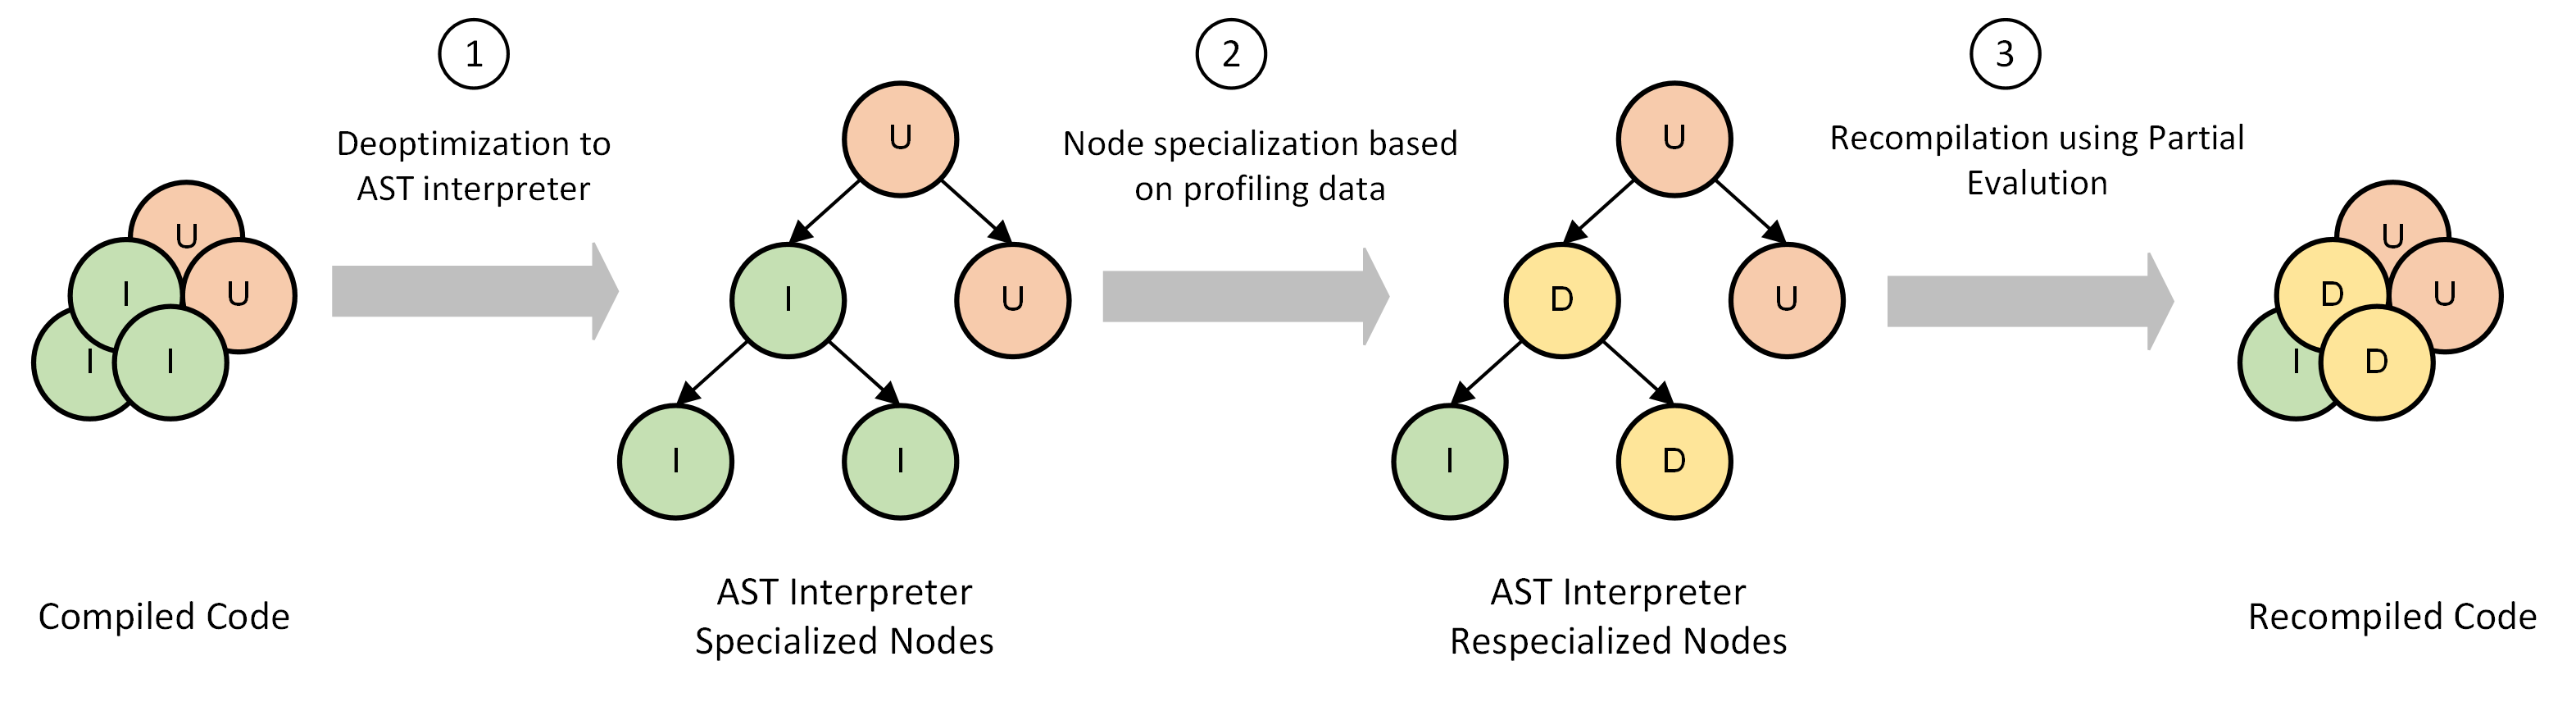
\includegraphics[width= 1\textwidth]{images/deoptimization-recompilation-pe.png}
    \caption{Jestliže spekulace stability stromu je porušena, dochází k~deoptimalizaci,  strojový kód je zahozen a AST strom se interpretuje {\Large \textcircled{\normalsize 1}}. Uzly se opět specializují na základě profilujících dat {\Large \textcircled{\normalsize 2}}, a~jakmile jsou podmínky pro JIT kompilaci znovu splněny, dochází k~další kompilaci do strojového kódu {\Large \textcircled{\normalsize 3}} \cite{one-vm-to-rule-them-all}}
    \label{fig:tree-deopt-and-respecilized}
\end{figure}


\clearpage


\subsection{Truffle DSL}
\label{truffle-dsl-chapter}
Sebeoptimalizace pomocí specializací je klíčovou částí frameworku Truffle. Přechod mezi jednotlivými specializacemi je velice repetitivní a náročný proces s~vysokou mírou pravděpodobnosti zanesení chyby. Tento problém je řešen pomocí Truffle DSL, což je anotační procesor využívající doménově specifický jazyk sloužící pro řízení přechodů mezi jednotlivými specializacemi. Ve zdrojovém kódu \ref{specialization-without-truffle-dsl} je možné vidět zjednodušený příklad, jak by mohla vypadat implementace sčítání čísel typu \texttt{integer} bez použití Truffle DSL. Třída obsahuje vlastnost \texttt{specializationState} označenou anotací \texttt{@CompilationFinal}, ve které je uloženo, jaká specializace je právě aktivní. Jakmile je na tento uzel aplikována PE, kód neaktivních specializací je eliminován. Jak je možné vidět z~implementace, kód pro sčítání dvou čísel typu \texttt{integer} je asi 30 řádků dlouhý, a přitom hlavní logika, kterou by se měl vývojář primárně zabývat, zabírá pouhý jeden řádek (sčítání dvou čísel je na řádku 33).  


\begin{listing} 
    \begin{minted}{java}
        public final class AdditionNode extends ExampleNode {
        @Child
        private ExampleNode leftNode, rightNode;
    
        private enum SpecializationState {UNINITIALIZED, INT, DOUBLE}
    
        @CompilationFinal
        private SpecializationState specializationState;
    
        ....
        
        @Override
        public int executeInt(VirtualFrame frame) throws UnexpectedResultException {
            int leftValue;
            try {
                leftValue = this.leftNode.executeInt(frame);
            } catch (UnexpectedResultException e) {
                this.activateDoubleSpecialization();
                double leftDouble = (double) e.getResult();
                throw new UnexpectedResultException(leftDouble + this.rightNode.executeDouble(frame));
            }
    
            int rightValue;
            try {
                rightValue = this.rightNode.executeInt(frame);
            } catch (UnexpectedResultException e) {
                this.activateDoubleSpecialization();
                double rightDouble = (double) e.getResult();
                throw new UnexpectedResultException(leftValue + rightDouble);
            }
    
            try {
                return Math.addExact(leftValue, rightValue);
            } catch (ArithmeticException e) {
                this.activateDoubleSpecialization();
                throw new UnexpectedResultException((double) leftValue + (double) rightValue);
            }
        }
    
        private void activateDoubleSpecialization() {
            this.specializationState = SpecializationState.DOUBLE;
        }
    
        // omitted other execute methods for simplicity
    \end{minted}
    \caption{Příklad implementace uzlu pro sčítání dvou čísel bez využití Truffle DSL \cite{specialization-intro-adam-ruka}}
    \label{specialization-without-truffle-dsl}
\end{listing}


Z~tohoto důvodu byl vytvořen Truffle DSL, který jednotlivé přechody mezi specializacemi vygeneruje, což nejen snižuje množství kódu, který vývojář musí během implementace interpretu napsat, ale i snižuje pravděpodobnost zanesení chyby. Další výhodou je fakt, že se vývojář zabývá pouze logikou dané specializace, a tím se zjednodušuje celý proces implementace dané operace. Ve zdrojovém kódu \ref{truffle-dsl-in-use} je možné vidět použití Truffle DSL na uzlu reprezentujícím operaci sčítání. Jelikož anotační procesor nesmí modifikovat existující třídy,\footnote{Standard anotačního procesoru Java zakazuje modifikaci existujících tříd. Projekt Lombok tento standard porušuje. \cite{lombok-adam-ruka}} musí být všechny třídy využívající Truffle DSL abstraktní. Během kompilace je pak vygenerována třída obsahující logiku jednotlivých specializací, včetně logiky starající se o~přechody mezi jednotlivými specializacemi. Jak je možné vidět ve zdrojovém kódu, potomci uzlu jsou v~tomto případě definováni pomocí anotace \texttt{@NodeChild}, která je sémanticky totožná s~anotací \texttt{@Child}. Stejně tak anotace \texttt{@Children} by byla nahrazena anotací \texttt{@NodeChildren}. Specializace jsou reprezentovány pomocí metod, které obsahují anotaci \texttt{@Specialization}. Pomocí atributu \texttt{rewriteOn} je pak možné specifikovat, kdy se má specializace deaktivovat. V~tomto případě specializace pro sčítání dvou čísel typu \texttt{integer} bude deaktivována, jakmile nastane \texttt{ArithmeticException} a bude nahrazena specializací pro sčítání čísel typu \texttt{double} (viz \texttt{replaces = "addInts"} na řádku 10 ve zdrojovém kódu \ref{truffle-dsl-in-use}). Nahrazení specializace za novou je zde možné pouze z~důvodu, že čísla typu \texttt{integer} jsou podmnožinou čísel typu \texttt{double}.


\begin{listing} 
    \begin{minted}{java}
        @NodeChild("leftNode") @NodeChild("rightNode")
        public abstract class AdditionNode extends SchemeExpression {
        
            @Specialization(rewriteOn = ArithmeticException.class)
            protected int addInts(int leftVal, int rightVal) {
                return Math.addExact(leftVal, rightVal);
            }
        
            @Specialization(replaces = "addInts")
            protected double addDoubles(double leftVal, double rightVal) {
                return leftVal + rightVal;
            }
        
            @Specialization
            protected String addStrings(String leftVal, String rightVal) {
                return leftVal + rightVal;
            }
        }
    \end{minted}
    \caption{Implementace uzlu pro sčítání dvou čísel s~využitím Truffle DSL}
    \label{truffle-dsl-in-use}
\end{listing}


\clearpage


\section{Scheme na platformě GraalVM}
\label{chapter-scheme-on-graalvm-platform}
Tato kapitola se bude zabývat popisem jednotlivých funkcionalit, které tato implementace jazyka Scheme podporuje (dále také nazývaná TruffleScheme). Jak již bylo zmíněno v~úvodní kapitole, cílem této práce nebylo implementovat co nejvíce ze specifikace jazyka Scheme, ale implementovat prvky, které dosud na platformě nebyly implementované a zároveň umožní vykonání benchmarkových testů.


\subsection{Datové typy}
V~této sekci jsou popsány všechny datové typy, které TruffleScheme podporuje. Zároveň je zmíněno, jak je každý interní typ reprezentován.

\begin{itemize}
    \item \textbf{Pravdivostní hodnota} je interně reprezentována jako Java \texttt{boolean}.
    \item \textbf{Celá čísla} jsou interně reprezentována jako Java \texttt{long}. V~případě, že datový typ \texttt{long} není dostačující, je využit \texttt{BigInteger}. Nutno zmínit, že třída \texttt{BigInteger} není použita přímo, ale je zapouzdřena do třídy nazývané \texttt{SchemeBigInt} z~důvodu podpory interoperability.
    \item \textbf{Čísla s~plovoucí desetinou čárkou} jsou interně reprezentována primitivní hodnotou \texttt{double}.
    \item \textbf{Symbol} je interně reprezentován třídou \texttt{SchemeSymbol}.
    \item \textbf{Řetězec} je interně reprezentován třídou \texttt{TruffleString} z~knihovny Truffle API. Implementace obsahuje funkce pro běžnou práci s~řetězcem, které na rozdíl od běžné Java implementace podporují partial evaluation.
    \item \textbf{List} je interně reprezentován třídou \texttt{SchemeList}. 
    \item \textbf{Tečkový pár} je interně reprezentován třídou \texttt{SchemePair}. 
    \item \textbf{Primitivní procedury} jsou interně reprezentovány třídou \texttt{Primitive\-Procedure}.
    \item \textbf{Uživatelsky definované procedury} jsou interně reprezentovány třídou \texttt{User\-Defined\-Procedure}.
    \item \textbf{Nedefinovaná hodnota} je interně reprezentována třídou \texttt{Undefined\-Value}. 
\end{itemize}


\subsection{Primitivní procedury} 
Primitivní procedury jsou základními stavebními bloky, které jsou programátorovi poskytnuty automaticky, bez nutnosti jejich definice. Všechny vazby mezi primitivní procedurou a symbolem jsou vytvořeny automaticky při startu interpretu v~globálním prostředí. Jedná se stejné vazby, které programátor může vytvořit, tudíž je lze redefinovat. Podporové primitivní procedury jsou: 

\begin{itemize}
    \item \textbf{Aritmetické:} +, -, *, /, modulo.
    \item \textbf{Porovnání čísel:} <, <=, >, >=, =.
    \item \textbf{Práce s~listem nebo párem:} car, cdr, cons, append, length, list.
    \item \textbf{Ostatní:} apply, map, not, null?, current-milliseconds, display.
\end{itemize}

\subsection{Speciální formy} 
Některé konstrukty jazyka nelze implementovat pomocí primitivních procedur. Například při definování nové vazby je důležité zajistit, aby symbol nebyl vyhodnocen před samotnou aplikací speciální formy. Vzhledem k~tomu, že primitivní procedury vyhodnocují všechny své argumenty před aplikací procedury, jsou potřeba nové elementy jazyka, které si budou samy řídit vyhodnocení jednotlivých argumentů. Speciální formy jsou právě těmito elementy jazyka. Tabulka~\ref{table-operators} vysvětluje význam operátorů, použitých pro definování gramatik jednotlivých speciálních forem. 


\begin{table}[ht]
\centering
\begin{tabular}{|c|c|}
    \hline
    \textbf{Operátor} & \textbf{Význam} \\
    \hline
    ? & 0 až 1 krát \\
    * & 0 až n krát \\
    + & 1 až n krát \\
    \hline
\end{tabular}
\caption{Význam operátorů použitých pro definovaní gramatik}
\label{table-operators}
\end{table}

Podporované speciální formy a jejich gramatiky jsou: 


\begin{itemize}
    \item \textbf{define}: \texttt{(define <jméno> <výraz>)}
    \item \textbf{lambda}: \texttt{(lambda (<param>*) <tělo>)} 
    \item \textbf{let}: \texttt{(let (<vazba>+) <tělo>)}
    \item \textbf{letrec}: \texttt{(letrec (<vazba>+) <tělo>)}
    \begin{itemize}
        \item kde \texttt{vazba}: \texttt{(symbol hodnota)}
    \end{itemize}
    % \begin{verbatim}
    %     (let ((<symbol_1> <hodnota_1>)
    %           (<symbol_2> <hodnota_2>)
    %           ...
    %           (<symbol_n> <hodnota_n>))
    %        <telo>)
    % \end{verbatim}
    % \item \textbf{letrec}: 
    % \begin{verbatim}
    %     (letrec ((<symbol_1> <hodnota_1>)
    %              (<symbol_2> <hodnota_2>)
    %              ...
    %              (<symbol_n> <hodnota_n>))
    %        <telo>)
    % \end{verbatim}
    \item \textbf{if}: \texttt{(if <test> <důsledek> <náhradník>?)}
    \item \textbf{and}: \texttt{(and <test>*)}
    \item \textbf{or}: \texttt{(or <test>*)}
    \item \textbf{quote}: \texttt{(quote <arg>)}
    \item \textbf{quasiquote}: \texttt{(quasiquote <arg>)}
    \item \textbf{define-macro}: \texttt{(define-macro <jméno> <výraz>)}
\end{itemize}


\subsection{Makra} 
\label{chapter-macros}
Jazyk Scheme umožňuje uživateli definovat vlastní speciální formy pomocí maker. Makra lze obecně rozdělit do dvou skupin, \textit{hygienická} a \textit{nehygienická}. Rozdíl spočívá v~tom, zda makro automaticky řeší konflikt jmen lokálních proměnných či parametrů. Jak je z~názvu zřejmé, hygienická makra tento problém řeší automaticky, naopak u~nehygienických maker se o~„hygienu“ musí postarat programátor sám. Hygienická makra je možné najít v~jazycích jako Rust, Julia či Dylan, naopak nehygienická makra je pak možné najít v~jazycích jako Clojure nebo Common Lisp. I~přesto, že ve specifikaci jazyka Scheme není zmínka o~nehygienických makrech, existuje mnoho implementací, které tyto makra podporují. Například implementace Racket podporuje nehygienická makra primárně z~důvodu kompatibility. Nevýhodou této implementace je fakt, že makro expanze nehygienických maker probíhá ve fázi nazývané \textit{expanze syntaxe}, ve které se nemohou využívat vazby definované uživatelem (jelikož tyto vazby ještě nevznikly). \cite{legacy-macro-support}

TruffleScheme implementuje pouze nehygienická makra, a to pomocí výše zmíněné speciální formy \texttt{define-macro}. To znamená, že každé makro musí obsahovat tzv. \textit{transformační proceduru}, což je procedura, jejíž výsledkem jsou data, která nahradí místo volání daného makra (to je možné, jelikož data lze chápat jako program, viz kapitola \ref{chapter-architecture-of-interpreter}). Tato transformace se často nazývá \textit{expanze maker}. Implementačními detaily maker se zabývá kapitola \ref{chapter-macros-implementation}.


\newpage
\section{Implementace interpretu}
V~této kapitole je nejprve popsána celková architektura interpretu včetně všech jeho částí a poté je popsána implementace základních prvků, jako jsou například primitivní procedury, speciální formy nebo uživatelsky definované procedury.  


\subsection{Architektura interpretu}
\label{chapter-architecture-of-interpreter}
Základní architekturu interpretu je možno vidět na obrázku \ref{fig:interpreter-architecture}. Vstupním argumentem je soubor obsahující zdrojový kód, který přijímá \texttt{parser}. Ten provádí lexikální a syntaktickou analýzu zdrojového kódu pomocí nástroje ANTLR.\footnote{ANTLR (ANother Tool for Language Recognition) je nástroj, který na základě definované gramatiky vygeneruje lexikální a syntaktický analyzátor. \cite{antlr}} Výsledkem je \textit{interní reprezentace} neboli vnitřní forma, což je způsob, kterým jsou reprezentována data {\Large \textcircled{\normalsize 1}}. Stejná data jsou pak výsledkem vyhodnocení výrazů.

\texttt{Converter} následně přijímá tuto interní reprezentaci (data) a transformuje je do abstraktních syntaktických stromů Truffle {\Large \textcircled{\normalsize 2}}. Tyto stromy jsou následně uloženy do \texttt{SchemeRootNode}, což je potomek \texttt{RootNode}, který reprezentuje kořen daného stromu. To znamená, že celý program si lze představit jako jeden velký abstraktní syntaktický strom Truffle (primitivní a uživatelsky definované procedury jsou samostatné abstraktní stromy, které jsou odtud volány), který je po konverzi vyhodnocen. Důležité je podotknout, že jakákoliv data lze transformovat na abstraktní syntaktické stromy Truffle, což znamená, že program lze chápat jako data nebo data lze chápat jako program. 



\begin{figure} [h]
    \centering
    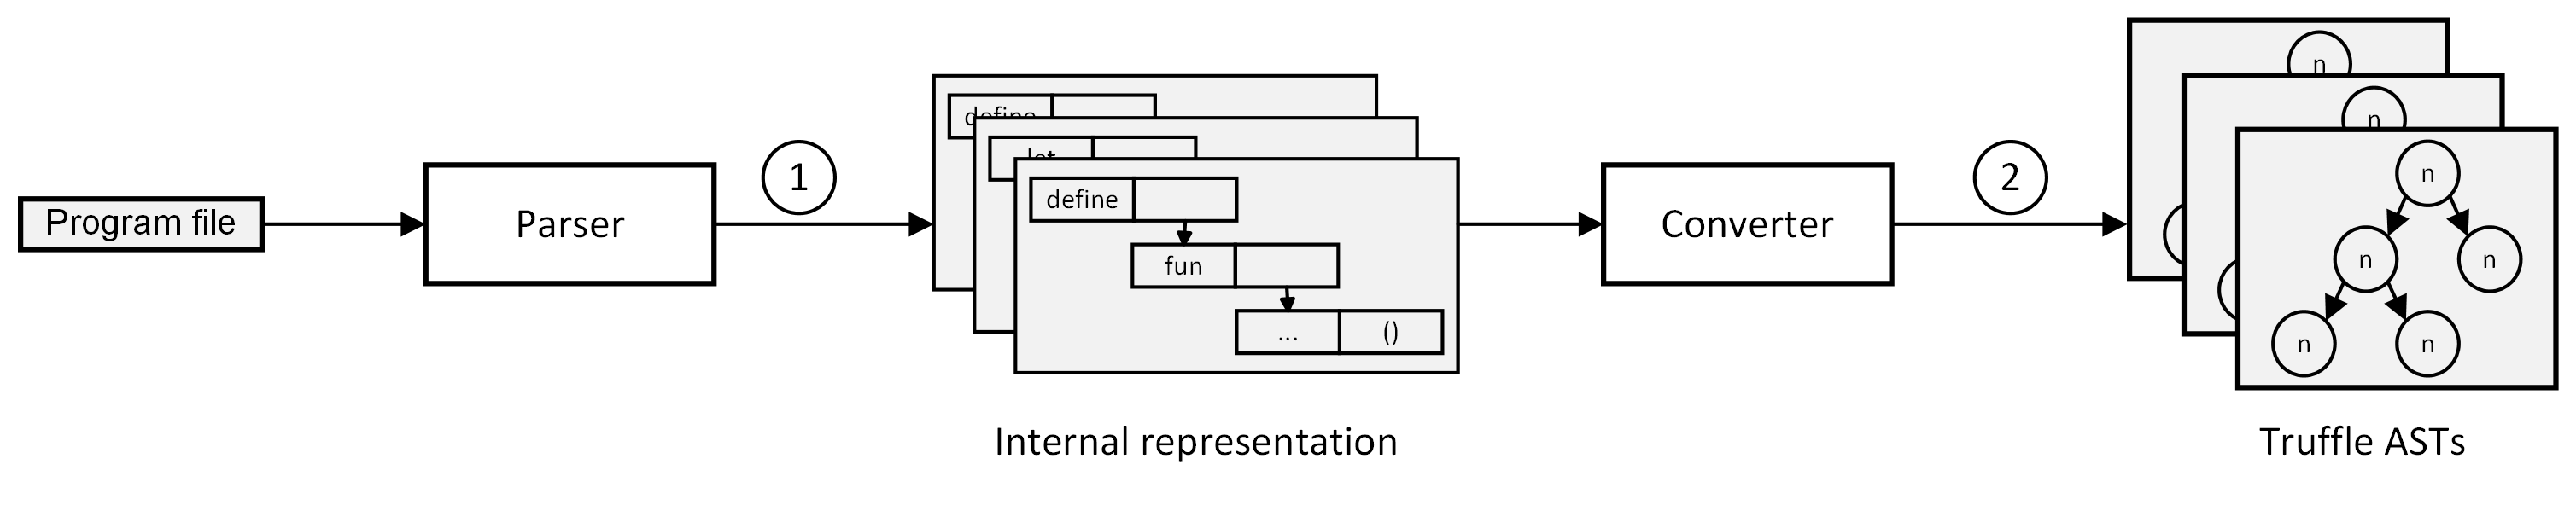
\includegraphics[width= 1\textwidth]{images/interpreter-architecture.png}
    \caption{Architektura interpretu}
    \label{fig:interpreter-architecture}
\end{figure}


\subsection{Lokální proměnné}
Jak již bylo zmíněno v~kapitole \ref{chapter-virtualFrame}, \texttt{VirtualFrame} slouží k~ukládaní lokálních proměnných. O~zapisování jednotlivých lokálních proměnných se stará uzel pojmenovaný \texttt{WriteFrameSlotNode}. Implementace tohoto uzlu (viz zdrojový kód \ref{WriteFrameSlotNode}) obsahuje hned několik prvků, které již byly popsány, ale nebyly demonstrovány na příkladu. První je vlastnost \texttt{guards} v~anotaci \texttt{@Specialization}, která je detailně popsána v~kapitole \ref{specialization-chapter}. Jedná se o~kontrolu, která se provádí před vykonáním samostatné specializace. Výraz, který se nachází v~kontrole (v~tomto případě volání funkce \texttt{isExpectedOrIllegal}) se musí vyhodnotit na \texttt{boolean} hodnotu. V~případě, že se výraz v~kontrole vyhodnotí na \texttt{true}, je specializace vykonána, v~opačném případě se přechází na další specializaci v~pořadí. Je důležité zmínit, že specializace se vykonávají v~pořadí, ve kterém jsou deklarovány ve zdrojovém kódu. Je proto vhodné, aby první specializace byla tou nejvíce pravděpodobnou a naopak poslední specializace byla tou nejméně pravděpodobnou (nebo generickou, která pokrývá celou sémantiku operace). V~tomto případě je možné vidět, že poslední specializace je generická, jelikož hodnota, kterou ukládáme, je typu \texttt{Object}, což je typ, na který lze v~Javě převést jakoukoliv jinou hodnotu. Dále stojí za povšimnutí, že tato generická specializace obsahuje vlastnost \texttt{replace}, která nahrazuje všechny předchozí specializace. Uzel se tak dostal do generického stavu a k~dalším specializacím již nedojde (viz podmínka konečnosti v~kapitole \ref{self-optimalization-of-ast-interpreters}).


Poslední zajímavostí je aktualizace \texttt{FrameDescriptoru}, kterou je možné vidět na řádku 33 ve zdrojovém kódu.\footnote{Aktualizace \texttt{FrameDescriptoru} probíhá i v~ostatních specializacích, a to v~metodě \texttt{isExpectedOrIllegal}, jejíž implementace z~důvodu stručnosti byla vynechána.} Na začátku má každá lokální proměnná nastavený typ na \texttt{Illegal} (odtud název funkce \texttt{isExpectedOrIllegal}), jelikož typ lokální proměnné není znám. Po prvním uložení hodnoty se \texttt{Frame\-Descriptor} aktualizuje a při dalším zavolání je vytvořen paměťově úspornější \texttt{VirtualFrame}. Pokud by lokální proměnná vždy nabývala hodnoty stejného typu, strojový kód vytvořený JIT kompilátorem by byl totožný se strojovým kódem staticky typovaného jazyka.

\begin{listing} 
    \begin{minted}{java}
        public abstract class WriteFrameSlotNode extends SchemeNode {
        
            @CompilationFinal
            private FrameDescriptor cachedDescriptor;
        
            private final int frameSlot;
        
            public abstract void executeWrite(VirtualFrame frame, Object value);
        
            public WriteFrameSlotNode(int frameSlot) {
                assert frameSlot >= 0;
                this.frameSlot = frameSlot;
            }
        
            @Specialization(guards = "isExpectedOrIllegal(frame, Long)")
            protected void writeLong(VirtualFrame frame, long value) {
                frame.setLong(frameSlot, value);
            }
            @Specialization(guards = "isExpectedOrIllegal(frame, Boolean)")
            protected void writeBoolean(VirtualFrame frame, boolean value) {
                frame.setBoolean(frameSlot, value);
            }
        
            @Specialization(guards = "isExpectedOrIllegal(frame, Double)")
            protected void writeDouble(VirtualFrame frame, double value) {
                frame.setDouble(frameSlot, value);
            }
        
            @Specialization(replaces = { "writeBoolean", "writeLong", "writeDouble" })
            protected void writeObject(VirtualFrame frame, Object value) {
                /* No-op if kind is already Object. */
                final FrameDescriptor descriptor = getFrameDescriptor(frame);
                descriptor.setSlotKind(frameSlot, FrameSlotKind.Object);
        
                frame.setObject(frameSlot, value);
            }
        
            //omitted for simplicity
    \end{minted}
    \caption{Uzel zapisující lokální proměnnou}
    \label{WriteFrameSlotNode}
\end{listing}


\clearpage


\subsection{Globální proměnné}
Globální proměnné se neukládají do \texttt{VirtualFramu}, ale do tzv. \textit{jazykového kontextu}, který je vytvořen při spuštění interpretu. To je zcela běžné v~jazycích implementovaných nad platformou GraalVM, a to z~důvodu podpory polyglotního programování. Dost často je nutné přistupovat do globálního prostředí cizího jazyku, a proto se musí jednat o~objekt, který podporuje interoperabilitu (což \texttt{VirtualFrame} není). Detailněji se problematikou interoperability zabývá kapitola \ref{chapter-interoperability-support}. 

Implementaci jazykového kontextu je možné vidět ve zdrojovém kódu \ref{SchemeLanguageContext}, kde třída obsahuje vlastnost \texttt{globalVariableStorage}, což je mapa, ve které jsou uloženy globální proměnné. Tato třída také poskytuje dvě metody pro přidávání a čtení globálních proměnných. Dále zdrojový kód obsahuje dva nové prvky, které dosud nebyly podrobně popsány.



První je anotace \texttt{@TruffleBoundary}, což je informace pro překladač Graal, aby na následující metodu neaplikoval partial evaluation. V~tomto případě na metody nemůže být aplikovaná partial evaluation, protože obsahují práci s~mapou, jejíž implementace (v~tomto případě implementace metod \texttt{put} a \texttt{get}) by způsobila vygenerování příliš mnoho strojového kódu (došlo by k~tzv. \textit{code explosion}).

Druhým prvkem je použití třídy \texttt{CyclicAssumption} z~knihovny Truffle~API, která umožňuje vytvářet vlastní spekulace. Ty jsou klíčovým prvkem sofistikovaných optimalizací. V~tomto případě je vytvořena spekulace, že globální proměnné jsou konstantní, a tudíž nebudou změněny. Tímto je možné při čtení globální proměnné hodnotu cachovat a výrazně tak zrychlit opětovné čtení těchto proměnných. Jak je možné vidět ve zdrojovém kódu \ref{SchemeLanguageContext} na řádku 28, spekulace je zneplatněna, jakmile dojde k~redefinici již definovaného symbolu. Kontrola, zda je spekulace validní a následné cachování hodnoty je implementováno ve třídě \texttt{ReadGlobalVariableExprNode}. 

Zajímavostí je, že kontrola, zda je spekulace stále validní není obsažena v~JIT zkompilovaném kódu, a to díky tomu, jak jsou spekulace ve frameworku Truffle implementovány. Řídí se tzv. \textit{hollywoodským principem}.\footnote{Hollywoodský princip je známý frází: \uv{\textit{Don't Call Us, We'll Call You}}. Čili kód nezjišťuje voláním, jestli je platný. Místo toho je mu to „sděleno“ připnutou spekulací.} Místo toho, aby byla prováděna kontrola, zda je spekulace validní před každým čtením globální proměnné, je sama spekulace „připnuta“ ke strojovému kódu, a~jakmile je spekulace zneplatněna, je zneplatněn i strojový kód. Kód je následně opět interpretován a nová spekulace muže být vytvořena (proto je použita třída \texttt{CyclicAssumption}, která automaticky po zneplatnění spekulace vytvoří novou).


\begin{listing} 
    \begin{minted}{java}
        public class SchemeLanguageContext implements TruffleObject {
        
            private final Map<SchemeSymbol, Object> globalVariableStorage;
            public static final CyclicAssumption notRedefinedAssumption = new CyclicAssumption("global variable not redefined");
            public final TruffleLanguage.Env env;
            private final PrintWriter output;
        
            public SchemeLanguageContext(TruffleLanguage.Env env) {
                this.globalVariableStorage = PrimitiveProcedureGenerator.generate();
                this.env = env;
                this.output = new PrintWriter(env.out(), true);
            }
        
            @TruffleBoundary
            public Object getVariable(SchemeSymbol symbol) {
                var value = globalVariableStorage.get(symbol);
                if (value == null) {
                    throw new SchemeException(symbol + ": undefined cannot reference an identifier before its definition", null);
                }
                return value;
            }
        
            @TruffleBoundary
            public void addVariable(SchemeSymbol symbol, Object valueToStore) {
                var shouldInvalidate = globalVariableStorage.containsKey(symbol);
                globalVariableStorage.put(symbol, valueToStore);
                if (shouldInvalidate) {
                    notRedefinedAssumption.invalidate();
                }
            }
             //omitted for simplicity
    \end{minted}
    \caption{Jazykový kontext obsahující mapu pro ukládání globálních proměnných}
    \label{SchemeLanguageContext}
\end{listing}


\clearpage


\subsection{Uživatelsky definované procedury}
\label{chapter-user-defined-procedures}
Uživatelsky definované procedury jsou v~jazyce Scheme \textit{elementy prvního řádu}. Každý element prvního řádu musí splňovat následující podmínky \cite{paradigmata-programovani1a}: 

\begin{itemize}
    \item Element může být pojmenován.
    \item Element může být předán proceduře jako argument.
    \item Element může vzniknout voláním jiné procedury.
    \item Element může být obsažen v~hierarchických datových strukturách. 
\end{itemize}


Uživatelsky definované procedury jsou ve frameworku Truffle reprezentované pomocí již zmíněného \texttt{CallTargetu} (viz kapitola \ref{chapter-callTarget}). Ten je zapouzdřen do třídy \texttt{UserDefinedProcedure}, což je interní reprezentace, která navíc obsahuje předpokládaný počet argumentů, lexikálního předka nebo jméno dané procedury. Při jejím volání jsou nejprve její argumenty uloženy jako lokální proměnné. To z~důvodu, že argumenty jsou předávány skrze pole typu \texttt{Object[]} (viz obrázek \ref{fig:argument-array}), což by mohlo zapříčinit neustálé \textit{boxování} a \textit{unboxování} vstupních argumentů.\footnote{Boxování (ang. boxing) je proces, při kterém se hodnota primitivního typu (např. \texttt{int}) převede na hodnotu objektového typu (např. \texttt{Integer}). Unboxování (ang. unboxing) je opačný proces, jedná se o~převod hodnoty z~objektového typu na primitivní typ.}


Ve výše zmíněním poli je první prvek vyhrazen lexikálnímu předku, tedy instanci třídy \texttt{VirtualFrame}, ve které byla procedura deklarována. Takto uložená instance musí být tzv. \textit{materializována}, jelikož nesmí zaniknout s~koncem volání procedury, se kterou byla vytvořena. Materializování \texttt{VirtualFramu} je drahá operace, a proto TruffleScheme implementuje optimalizaci, která během parsování detekuje, zda procedura vyžaduje lexikálního předka. Pokud nevyžaduje, lexikální předek je nahrazen hodnotou \texttt{null}.


\begin{figure} [h]
    \centering
    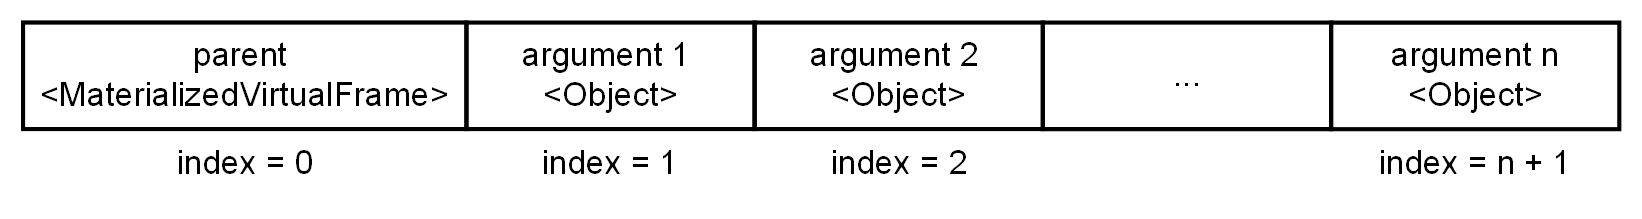
\includegraphics[width= 1\textwidth]{images/argument-array.png}
    \caption{Pole argumentů při volání procedury. Argument na indexu \texttt{i} se získá pomocí vzorce \texttt{i + 1} }
    \label{fig:argument-array}
\end{figure}

I~přesto, že \texttt{CallTarget} obsahuje metodu \texttt{call}, není optimální takto procedury volat. Jakékoliv volání \texttt{CallTargetu} by mělo být provedeno skrze uzly \texttt{DirectCallNode} nebo \texttt{IndirectCallNode}.\footnote{\texttt{DirectCallNode} a \texttt{IndirectCallNode} jsou součástí knihovny Truffle API.} Jak je patrné z~názvu, výběr konkrétního uzlu závisí na stabilitě \texttt{CallTargetu}.

\texttt{DirectCallNode} se používá v~případě, že \texttt{CallTarget} je statický, což znamená, že se procedura vyhodnotí vždy na stejnou proceduru ve stejném \textit{místě volání} (ang. call site). Naopak \texttt{IndirectCallNode} se používá v~případě, že \texttt{CallTarget} je dynamický, a tudíž se procedura může vyhodnotit na jinou proceduru ve stejném místě volání. To je typické pro případy, kdy je procedura argumentem jiné procedury, což je v~jazyku Scheme zcela běžné. 

Pokud je procedura volána skrze \texttt{DirectCallNode}, platforma GraalVM je pak schopná provést následující optimalizace: 

\begin{itemize}
    \item Eliminace volání metod (ang. method inlining).
    \item Duplikaci abstraktního syntaktického stromu Truffle s~ohledem na místo volání procedury (ang. call site sensitive AST duplication).
\end{itemize}


První zmíněná optimalizace byla popsána v~kapitole \ref{jit-optimalizations}. V~Truffle kontextu se jedná o~optimalizaci, kde abstraktní syntaktický strom Truffle uložený v~\texttt{CallTargetu} je vložen do \texttt{CallTargetu} předka. Tato optimalizace probíhá nad Graal IR. To znamená, že ve výsledném grafu bude uzel reprezentující volání procedury nahrazen grafem reprezentující tělo eliminované procedury.  

Druhá zmíněná optimalizace vytváří novou kopii \texttt{CallTargetu} v~neinicializovaném stavu. Tato optimalizace se využívá, jakmile Truffle detekuje, že se procedura volá z~více různých míst, kde na každém místě se využívají jiné specializace (polymorfní volání). Originální \texttt{CallTarget} pak zůstává v~polymorfní podobě, ale nově vytvořená kopie se následně specializuje na základě profilujících dat z~nového místa volání (je proto vysoká pravděpodobnost, že nový \texttt{CallTarget} bude monomorfní). 

 
Naopak pokud je procedura volána skrze \texttt{IndirectCallNode}, GraalVM nemůže provést žádnou výše zmíněnou optimalizaci. Ale i přesto dochází v~tomto uzlu k~profilování typů vstupních argumentů, což posléze umožní eliminovat mnoho typových kontrol (například u~specializací), jelikož typ jednotlivých argumentů je považován za konstantní. Stejné profilování samozřejmě probíhá i~u~\texttt{DirectCallNode}.


TruffleScheme využívá uzel \texttt{DispatchUserProcedureNode} k~volání uživatelsky definovaných procedur, jehož implementaci je možno vidět ve zdrojovém kódu \ref{DispatchUserProcedureNode}. Tento zdrojový kód využívá dva nové prvky, které dosud nebyly popsány. Jedná se o~anotaci \texttt{@Cached} a s~ní spojený atribut \texttt{limit}. Anotace \texttt{@Cached} se používá k~definovaní konstanty, která je spojená s~instancí dané specializace. Konstanta je vytvořena na základě výrazu, který je možno napsat do závorek k~anotaci. Pokud výraz není zadán (možné vidět na řádku 25 ve zdrojovém kódu) anotace se bude snažit vyhledat statickou metodu \texttt{create()} ve třídě, jejíhož typu je vytvářená konstanta.\footnote{Pokud se samozřejmě nejedná o~primitivní typ, ten je vytvořen triviálně.} Konstanty jsou vytvořeny ještě před vyhodnocením kontroly dané specializace, a tudíž je lze použít ve vlastnosti \texttt{guards} anotace \texttt{@Specialization}. Pokud tak vývojář učiní, musí pak definovat atribut \texttt{limit}, který specifikuje, kolik instancí dané specializace se může vytvořit. Vzniká tak stejně, jako v~případě řetězení specializací, polymorfní inline cache (viz kapitola \ref{specializations-and-performance}). Nutné zmínit, že pokud argument obsahující anotaci \texttt{@Cached} dědí z~třídy \texttt{Node}, je vytvořen nový potomek (tzn. že ve vygenerovaném kódu bude vlastnost obsahovat anotaci \texttt{@Child}), naopak pokud se jedná například o~argument primitivního typu, ve vygenerovaném kódu bude vlastnost obsahovat anotaci \texttt{@CompilationFinal}. 

To znamená, že v~případě \texttt{DispatchUserProcedureNode}, každé místo volání smí zavolat pouze tři různé procedury (jelikož \texttt{limit = 3}). Pokud je tento počet překročen, je metoda specializace \texttt{doCached} nahrazena generickou specializací \texttt{doUncached}, která je ovšem výrazně pomalejší.

\begin{listing} [H]
    \begin{minted}{java}
        public abstract class DispatchUserProcedureNode extends SchemeNode {
        
            public abstract Object executeDispatch(Object procedure, Object[] arguments);
        
            @Specialization(guards = "proc.callTarget() == procCached.callTarget()", limit = "3")
            protected static Object doCached(
                    UserDefinedProcedure proc,
                    Object[] arguments,
                    @Cached("proc") UserDefinedProcedure procCached,
                    @Cached("create(procCached.callTarget())") DirectCallNode directCallNode) {
                var argumentSize = arguments.length - 1;
                if (argumentSize != procCached.expectedNumberOfArgs()) {
                    CompilerDirectives.transferToInterpreterAndInvalidate();
                    throw SchemeException.arityException(null, procCached.name(), procCached.expectedNumberOfArgs(), argumentSize);
                }
                return directCallNode.call(arguments);
            }
        
            @Specialization(replaces = "doCached")
            protected static Object doUncached(
                    UserDefinedProcedure proc,
                    Object[] arguments,
                    @Cached IndirectCallNode indirectCallNode) {
                return indirectCallNode.call(proc.callTarget(), arguments);
            }
        }
    \end{minted}
    \caption{Uzel volající uživatelsky definované procedury}
    \label{DispatchUserProcedureNode}
\end{listing}



\subsection{Primitivní procedury}
Primitivní procedury by bylo možné implementovat stejně jako uživatelsky definované procedury, aniž by to ovlivnilo korektnost interpretu. Výsledky benchmarků by byly ve většině případů stejné, a to díky optimalizacím, které framework Truffle automaticky provádí (např. eliminace volání metod nebo duplikaci abstraktního syntaktického stromu Truffle). Problém by však mohl nastat, jakmile by byla interpretována větší aplikace. Každý JIT překladač má nějaký \textit{limit} (ang. budget), který může strávit na optimalizacích. 
Ve většině případů se jedná o~množství zdrojů (ang. resources), které překladač na optimalizace může využít. Překladač se pak snaží hledat nějaký kompromis mezi množstvím prostředků využitých na danou optimalizaci a benefity získanými touto optimalizací. Proto jsou primitivní procedury implementovány jiným způsobem, který se snaží co nejvíce JIT překladači „ulehčit“ práci.


Na rozdíl od uživatelsky definovaných procedur, primitivní procedury neobsahují \texttt{CallTarget} ve své interní reprezentaci. Obsahují tzv. \textit{továrnu} (ang. factory), která umí vytvořit abstraktní syntaktický strom Truffle, který reprezentuje tělo primitivní procedury. Primitivní procedury jsou volány skrze uzel \texttt{DispatchPrimitiveProcedureNode}, jehož implementaci můžeme vidět ve zdrojovém kódu \ref{DispatchPrimitiveProcedureNode}. Klíčový je zde řádek 11,  který vytvoří nového potomka typu \texttt{AlwaysInlinableProcedureNode} pomocí anotace \texttt{@Cached}, což je potomek reprezentující primitivní proceduru. Důležité je podotknout, co je dosaženo touto implementací. Každé místo volání při prvním provedení primitivní procedury vytvoří nového potomka, který je následně vyhodnocen. Při opětovném volání je pak pouze provedena kontrola, zda místo volání tuto instanci primitivní procedury již vidělo a v~případě že ano, dojde k~pouhému vyhodnocení již vzniklého potomka. V~případě, že se instance liší (jedná se o~jinou primitivní proceduru), je nastaven atribut \texttt{limit} na hodnotu 2, tudíž by vznikl další potomek, který by byl následně vyhodnocen. Pokud by místo volání zaznamenalo ještě jinou primitivní proceduru, byla by specializace zneplatněna a využívala by se generická specializace \texttt{doPrimitiveProcedureUncached}, která je samozřejmě pomalejší. To znamená, že touto implementací jsme de facto dosáhli optimalizací, které by JIT překladač musel dělat v~případě, že by se jednalo o~klasické volání procedur. Bylo eliminováno volání primitivní procedury a zároveň došlo i k~duplikaci abstraktního syntaktického stromu Truffle, jelikož v~každém místě volání je vytvořeno nové tělo primitivní procedury.  


\begin{listing} [H]
    \begin{minted}{java}
        public abstract class DispatchPrimitiveProcedureNode extends SchemeNode {
        
            public abstract Object execute(PrimitiveProcedure procedure, Object[] arguments);
        
        
            @Specialization(guards = "proc == procCached", limit = "2")
            protected static Object doPrimitiveProcedureCached(
                    PrimitiveProcedure pr,
                    Object[] arguments,
                    @Cached("proc") PrimitiveProcedure procCached,
                    @Cached("createInlinableNode(procCached)") AlwaysInlinableProcedureNode inlinedMethodNode) {
                return inlinedMethodNode.execute(arguments);
            }
        
            @Specialization(replaces = "doPrimitiveProcedureCached")
            protected static Object doPrimitiveProcedureUncached(
                    PrimitiveProcedure proc,
                    Object[] args) {
                return proc.factory().getUncachedInstance().execute(args);
            }
        
        
            protected static AlwaysInlinableProcedureNode createInlinableNode(PrimitiveProcedure procedure) {
                return procedure.factory().createNode();
            }
        }
    \end{minted}
    \caption{Uzel volající primitivní procedury}
    \label{DispatchPrimitiveProcedureNode}
\end{listing}


\subsection{Speciální formy}
Implementace speciálních forem je z~teoretického hlediska velice podobná primitivním procedurám. V~obou případech je eliminováno jakékoliv volání procedur. To je žádoucí, jelikož nejen že volání procedur s~sebou nese značnou režii, ale při volání procedur vzniká \texttt{VirtualFrame}, kterým je reprezentovaný lexikální předek, kterého primitivní procedury a některé speciální formy vůbec nepotřebují. 

TruffleScheme dokonce implementuje všechny podporované speciální formy bez nutnosti vytvoření nového \texttt{VirtualFrame}. To se na první pohled může zdát překvapivé, zejména u~speciálních forem jako let nebo letrec. Tyto formy nevytvářejí \texttt{VirtualFrame}, ale místo toho využívají \texttt{VirtualFrame}, ve kterém byly vyhodnoceny. Pokud je například použita speciální forma let uvnitř těla uživatelsky definované procedury, vazby speciální formy se uloží do \texttt{VirtualFramu} této procedury. Tímto se eliminuje nutnost tvory nového \texttt{VirtualFramu}.

Speciální formy jsou tvořeny během konverze interní reprezentace do abstraktních syntaktických stromů Truffle. Pokud se například při konverzi narazí na list, který obsahuje jako první prvek symbol \texttt{if}, je tento list vnímán jako volání speciální formy a je vytvořen uzel \texttt{IfExprNode}.\footnote{Uzel \texttt{IfExprNode} je samozřejmě vytvořen jen v~případě, že list reprezentující volání speciální formy \texttt{if} má velikost 3 (neobsahuje náhradníka). V~případě, že by náhradník byl součástí listu, je vytvořen uzel \texttt{IfElseExprNode}. Rozdělení operace na více uzlů je žádoucí, jelikož je tímto eliminováno větvení, které by bylo potřeba provést za běhu programu.} Jak je možné vidět ze zdrojového kódu \ref{IfExprNode}, uzel neobsahuje žádný mechanismus k~detekci, zda vazba speciální formy nebyla přepsána. Důvodem je fakt, že TruffleScheme nepodporuje redefinici speciálních forem. V~případě, že se o~to uživatel pokusí, je vyhozena výjimka. I~přesto, že by podpora redefinice nebyla příliš náročná na implementaci, benefit získaný touto podporou by byl minimální. 

\begin{listing} [H]
    \begin{minted}{java}
        public abstract class IfExprNode extends SchemeExpression {
    
            @Child private SchemeExpression condition;
            @Child private SchemeExpression thenExpr;
            
            public IfExprNode(SchemeExpression condition, SchemeExpression thenExpr) {
                this.condition = condition;
                this.thenExpr = thenExpr;
            }
    
            @Specialization
            protected Object doIf(VirtualFrame frame,
                                  @Cached BooleanCastNode cast,
                                  @Cached("createCountingProfile()") ConditionProfile condProfile) {
                final var conditionAsBool = cast.executeBoolean(condition.executeGeneric(frame));
                if (condProfile.profile(conditionAsBool)) {
                    return thenExpr.executeGeneric(frame);
                } else {
                    return UndefinedValue.SINGLETON;
                }
            }
        }
    \end{minted}
    \caption{Uzel reprezentující speciální formu \texttt{if}, která neobsahuje náhradníka}
    \label{IfExprNode}
\end{listing}



\subsection{Makra}
\label{chapter-macros-implementation}
Jak již bylo popsáno v~kapitole \ref{chapter-macros}, TruffleScheme implementuje pouze nehygienická makra, která lze definovat pomocí speciální formy \texttt{define-macro}. Tělo této speciální formy musí obsahovat výraz, který se vyhodnotí na uživatelsky definovanou proceduru. Tato procedura pak reprezentuje transformační proceduru makra. Jelikož není možné během konverze určit, zda se výraz vyhodnotí na proceduru, je nejprve tento výraz spolu se jménem daného makra uložen do konverzního kontextu.\footnote{Během konverze je vytvořen kontext, ve kterém jsou uloženy informace jako například lokální proměnné, makra nebo lexikální předek.} Jakmile dojde k~volání tohoto makra, je vytvořen uzel \texttt{MacroCallableExprNode}, který obsahuje jako potomka výraz, který byl pro dané makro uložený v~konverzním kontextu. Implementaci je možno vidět ve~zdrojovém kódu \ref{MacroCallableExprNode}. Při interpretaci tohoto uzlu nejprve dojde k~vyhodnocení potomka reprezentujícího transformační proceduru. V~případě, že se nevyhodnotí na uživatelsky definovanou proceduru, je vyhozena výjimka. Tento případ by znamenal, že speciální forma \texttt{define-macro} neobsahuje transformační proceduru. Kontrola, zda se potomkem vyhodnotil na uživatelsky definovanou proceduru, je v~tomto případě realizována pomocí anotace \texttt{@Fallback}, která obsahuje negované kontroly všech specializací definovaných v~daném uzlu. V~tomto případě uzel obsahuje jen jednu specializaci s~implicitní kontrolou, zda potomek je typu \texttt{UserDefinedProcedure}, což znamená, že metoda \texttt{fallback} bude přijímat všechny objekty, které nejsou typu \texttt{UserDefinedProcedure}.

V~případě, že se jedná o~uživatelsky definovanou proceduru, je standardně volána skrze uzel \texttt{DispatchUserProcedureNode}. Výsledkem tohoto volání jsou data, která jsou pomocí třídy \texttt{InternalRepresentationConverter} převedena na abstraktní syntaktický strom Truffle. Tento strom následně nahradí stávající uzel (tj. uzel \texttt{MacroCallableExprNode}) pomocí funkce \texttt{replace} (řádek 23 ve zdrojovém kódu \ref{MacroCallableExprNode}). Makro expanze tak probíhá při prvním volání makra, což znamená, že po tomto volání běhové prostředí již neobsahuje žádné známky maker. Bylo tak odstraněno i omezení týkající se využití uživatelsky definovaných vazeb během makro expanze (viz kapitola \ref{chapter-macros}). Jelikož je makro expanze prováděna při prvním volání makra, vazby již existují, a tudíž je možné tyto vazby využít.


\begin{listing} 
    \begin{minted}{java}
        public abstract class MacroCallableExprNode extends SchemeExpression {
    
            private final Object[] notEvalArgs;
            private final ConverterContext converterContext;
            private final SchemeSymbol name;
            @Child @Executed
            protected SchemeExpression transformationExpr;
    
            //constructor omitted
    
            @Specialization
            protected Object doMacroExpansion(
                    VirtualFrame frame,
                    UserDefinedProcedure proc,
                    @Cached DispatchUserProcedureNode dispatch) {
                CompilerDirectives.transferToInterpreterAndInvalidate();
                if (proc.expectedNumberOfArgs() != notEvalArgs.length) {
                    throw SchemeException.arityException(this, name.value(), proc.expectedNumberOfArgs(), notEvalArgs.length);
                }
    
                var args = getArgumentsForMacroExpansion(proc);
                var macroExpandedIR = dispatch.executeDispatch(proc, args);
                var macroExpandedAST = InternalRepresentationConverter.convert(macroExpandedIR, converterContext, false, false, null);
                return replace(macroExpandedAST).executeGeneric(frame);
            }
    
            @TruffleBoundary
            @Fallback
            Object fallback(Object object) {
                throw new SchemeException("""
                        macro's body has to be evaluated to procedure
                        expected: procedure?
                        given: %s""".formatted(object), this);
            }
    
            //omitted for simplicity
        }
    \end{minted}
    \caption{Uzel reprezentující volání makra}
    \label{MacroCallableExprNode}
\end{listing}


\clearpage


\subsection{Optimalizace koncových volání}
I~přesto, že jazyk Scheme obsahuje konstrukce pro tvorbu cyklů nebo smyček, jsou tyto konstrukce často nahrazovány rekurzivním voláním procedur, protože eliminují vedlejší efekt,\footnote{Vedlejší efekt (též vedlejší účinek, ang. side effect) je situace, kdy funkce nebo výpočetní výraz mění i jiný stav procesu, než je návratová hodnota funkce nebo změna hodnoty parametru odkazovaného přes odkaz referencí \cite{side-effect}.} který je častým zdrojem chyb. I~když jsou oba způsoby sémanticky totožné, rekurzivně volané procedury zabírají určité místo na zásobníku. Pokud by počet rekurzivně volaných procedur byl příliš vysoký, došlo by k~tzv. \textit{přetečení zásobníku} (ang. Stack overflow), což znamená, že velikost zásobníku překročila maximální povolenou velikost. Proto většina funkcionálních jazyků implementuje tzv. \textit{optimalizaci koncových volání} (ang. tail call optimalization), která je aplikována v~případě, že procedura je volaná z~tzv. \textit{koncové pozice} lambda výrazu. 

\begin{definition}[Koncová pozice]
Výraz je v~koncové pozici lambda výrazu $\Lambda$ v~případě, že splňuje alespoň jednu následující podmínku \cite{paradigmata-programovani1b}: 

\begin{enumerate}
    \item Poslední výraz v~těle výrazu $\Lambda$ je v koncové pozici výrazu $\Lambda$.
    \item Je-li \texttt{(if <test> <důsledek> <náhradník>?)} v~koncové pozici výrazu $\Lambda$, pak \texttt{<důsledek>} i \texttt{<náhradník>} jsou v~koncové pozici.
    \item Je-li \texttt{(and <test\textsubscript{1}> ... <test\textsubscript{n}>)} v~koncové pozici výrazu $\Lambda$, pak \texttt{<test\textsubscript{n}>} je v~koncové pozici. Obdobné platí i pro speciální formu \texttt{or}.
    \item Je-li \texttt{(let (<vazba>+) <výraz\textsubscript{1}> ... <výraz\textsubscript{n}>)} v~koncové pozici výrazu $\Lambda$, pak \texttt{<výraz\textsubscript{n}>} je v~koncové pozici. Obdobné platí i pro speciální formu \texttt{letrec}.
\end{enumerate}
\end{definition}


TruffleScheme implementace rozlišuje dvě varianty, které mohou nastat při aplikaci procedury v~koncové pozici. Pokud aplikovaná procedura je stejná jako procedura, která ji volá (jinými slovy procedura volá sama sebe v~koncové pozici), jedná se o~tzv. \textit{koncovou rekurzi}. Naopak pokud aplikovaná procedura je odlišná od procedury, která ji volá, jedná se o~klasické \textit{koncové volání}. TruffleScheme optimalizuje každou z~variant odlišně. 

Před popisem jednotlivých optimalizací je nejprve potřeba popsat obecnou techniku, ze které implementace vychází v~obou případech. Jedná se o~techniku zvanou \textit{trampolína}. Trampolína je ve své podstatě vnější procedura, která opakovaně volá vnitřní procedury v~koncové pozici. Pokud vnitřní procedura chce zavolat jinou proceduru v~koncové pozici, namísto jejího zavolání je tato procedura vrácena vnější proceduře (trampolíně), která ji následně zavolá. Tímto je eliminován problém přetečení zásobníku, jelikož v~tomto případě je velikost zásobníku konstantní. Rozdíl ve velikosti zásobníku je možné vidět na obrázku~\ref{fig:growing-stack-height}~a~\ref{fig:constant-stack-height}, kde je volána procedura \texttt{trampoline}, která reprezentuje onu vnější proceduru (trampolínu). Procedury \texttt{foo}, \texttt{bar} a \texttt{baz} pak reprezentují vnitřní procedury, které postupně budou volány procedurou \texttt{trampoline}. Implementaci procedury \texttt{trampoline} je možné vidět ve zdrojovém kódu \ref{tail-call-example}. \cite{trampile-jvm-elimination-techniques}

Jak již bylo zmíněno na začátku této kapitoly, TruffleScheme rozlišuje mezi koncovou rekurzí a koncovým voláním. V~následující kapitole bude nejprve popsána implementace koncové rekurze, kterou je možné chápat jako speciální případ koncového volání. Poté bude následovat kapitola popisující implementaci koncového volání.


\begin{figure} [h]
    \centering
    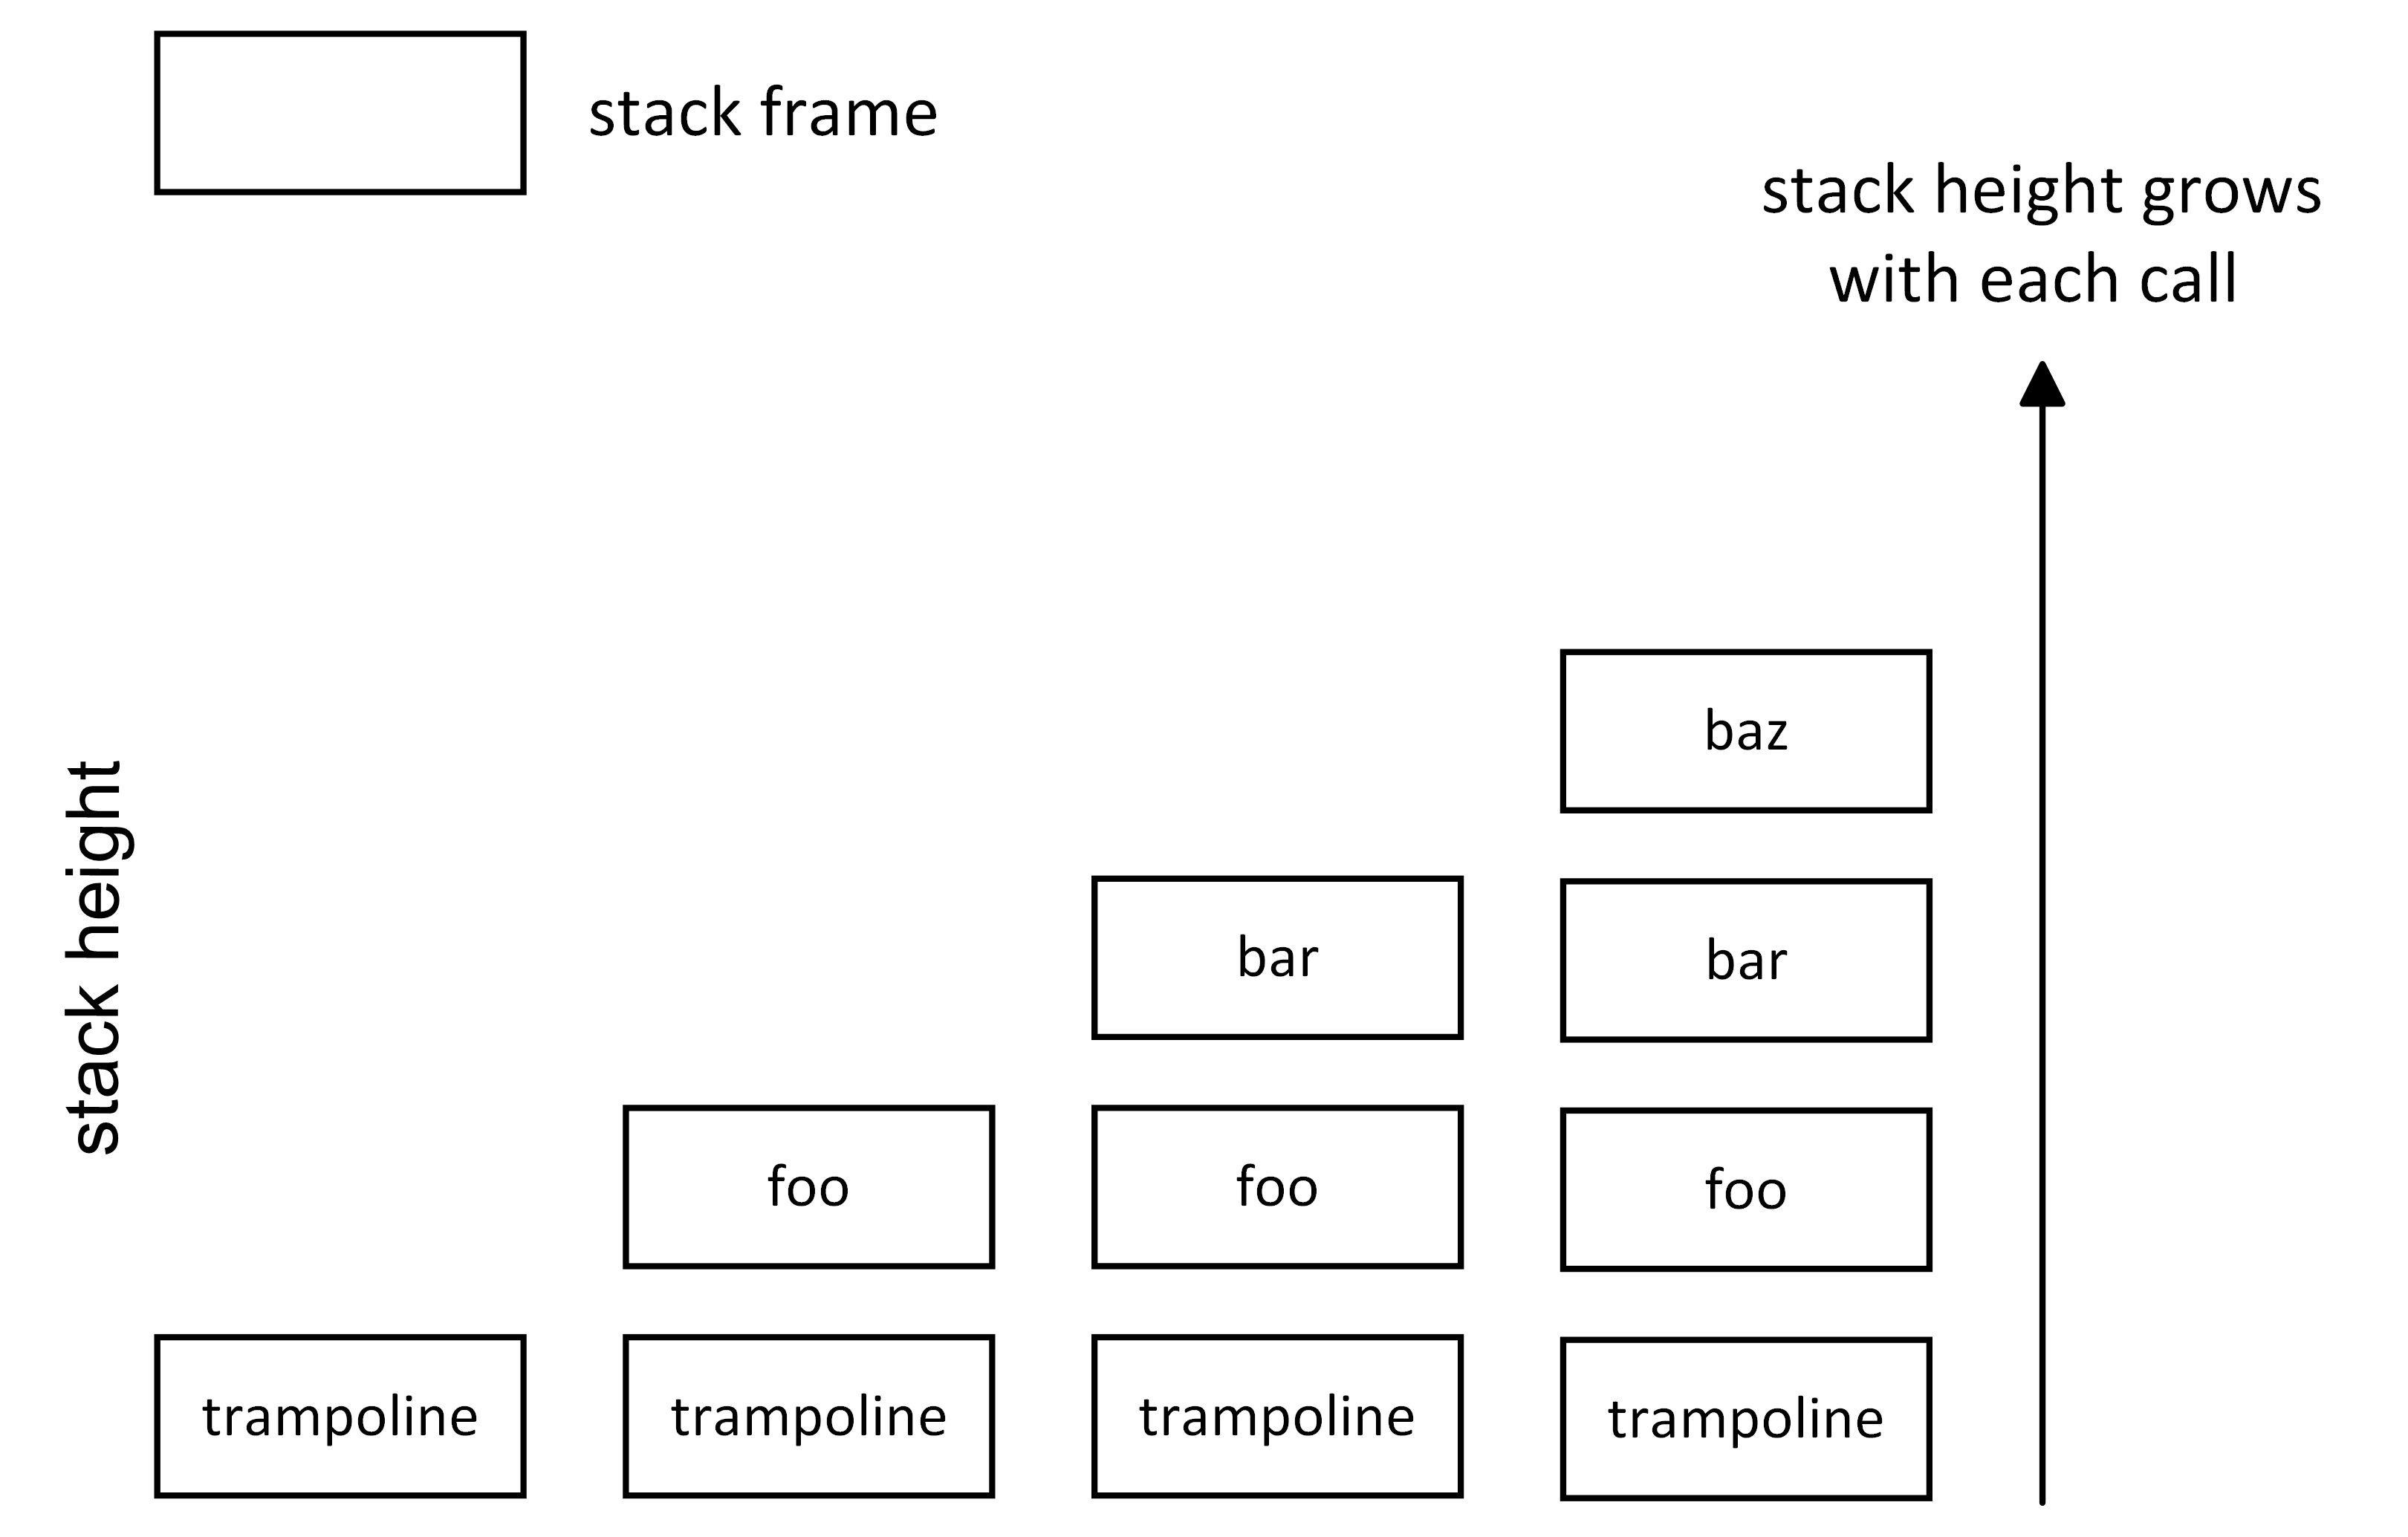
\includegraphics[width= 1\textwidth]{images/stack_frame.png}
    \caption{Velikosti zásobníku roste s~každým dalším voláním procedury v~případě, že není aplikována optimalizace koncových volání \cite{truffle-clojure}}
    \label{fig:growing-stack-height}
\end{figure}

\begin{figure} [h]
    \centering
    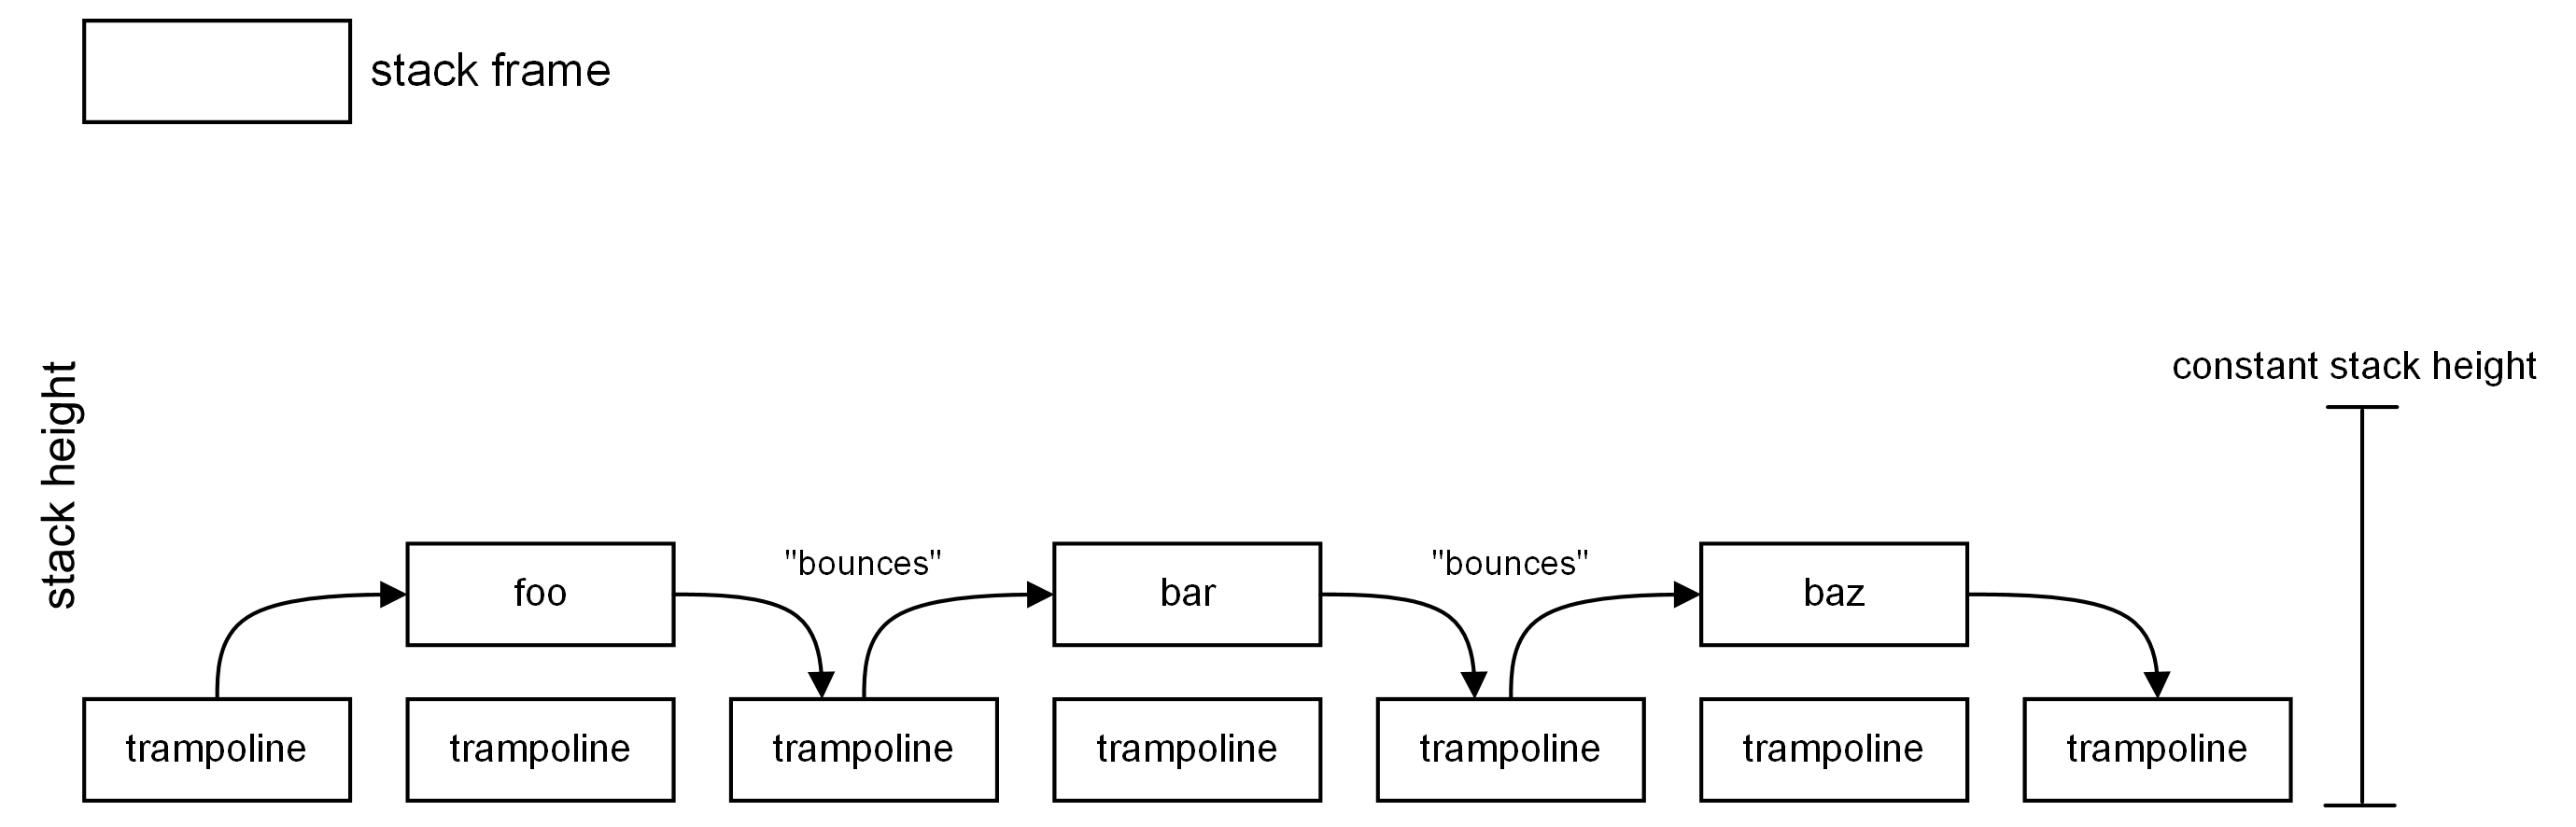
\includegraphics[width= 1\textwidth]{images/trampoline-bounce.png}
    \caption{Velikost zásobníku je konstantní s~každým dalším voláním procedury, v~případě, že je aplikována optimalizace koncových volání \cite{truffle-clojure}}
    \label{fig:constant-stack-height}
\end{figure}

\begin{listing} 
    \begin{minted}{scheme}
        (define trampoline
          (lambda ()
            (foo)))
        
        (define foo
          (lambda ()
            (bar)))
        
        (define bar
          (lambda ()
            (baz)))
        
        (define baz
          (lambda ()
            10))
        
        (trampoline)
    \end{minted}
    \caption{Procedura \texttt{trampoline} v~tomto případě bude sloužit jako trampolína (vnější procedura), která postupně bude volat vnitřní procedury \texttt{foo}, \texttt{bar} a \texttt{baz}}
    \label{tail-call-example}
\end{listing}



\subsubsection{Implementace optimalizace koncové rekurze}
Detekce koncové rekurze probíhá během konverze interní reprezentace na abstraktní syntaktické stromy Truffle. Pokud je zjištěno, že posledním výrazem v~těle právě definované procedury je volání stejnojmenné procedury, je toto volání nahrazeno speciálním uzlem \texttt{TailRecursiveThrowerNode}, jehož implementaci je možné vidět ve zdrojovém kódu \ref{TailRecursiveThrowerNode}. Z~této implementace je možné vidět, že nejprve jsou vyhodnoceny všechny argumenty procedury, poté jsou uloženy do \texttt{VirtualFramu} a následně je vyhozena výjimka \texttt{TailRecursiveException}. Tato výjimka je potomkem třídy \texttt{ControlFlowException}, což je speciální typ výjimky, kterou překladač Graal ve zkompilovaném kódu dokáže odstranit. Dále může být překvapivé, že výjimka neobsahuje žádná data, jako například proceduru, kterou vnější procedura bude volat. Je důležité si uvědomit, že díky tomu, že se jedná o~koncovou rekurzi, je tato procedura známa. Jedná se o~stejnou proceduru, která je právě volána.

\begin{listing} 
    \begin{minted}{java}
        public abstract class TailRecursiveThrowerNode extends SchemeExpression {
        
            @Children
            private final SchemeExpression[] arguments;
        
            @Children
            private final WriteFrameSlotNode[] writeFrameSlotNodes;
        
        
            public TailRecursiveThrowerNode(List<SchemeExpression> arguments, List<WriteFrameSlotNode> writeFrameSlotNodes) {
                this.arguments = arguments.toArray(SchemeExpression[]::new);
                this.writeFrameSlotNodes = writeFrameSlotNodes.toArray(WriteFrameSlotNode[]::new);
            }
        
            @Specialization
            protected Object doThrow(VirtualFrame frame) {
                prepareArguments(frame);
                throw TailRecursiveException.INSTANCE;
            }
        
        
            @ExplodeLoop
            private void prepareArguments(VirtualFrame frame) {
                Object[] evalArgs = new Object[arguments.length];
        
                for (int i = 0; i < arguments.length; i++) {
                    evalArgs[i] = arguments[i].executeGeneric(frame);
                }
        
                for (int i = 0; i < writeFrameSlotNodes.length; i++) {
                    writeFrameSlotNodes[i].executeWrite(frame, evalArgs[i]);
                }
            }
        }
    \end{minted}
    \caption{Uzel, který místo volání procedury vyhodí výjimku}
    \label{TailRecursiveThrowerNode}
\end{listing}



Výjimka je následně odchycena v~uzlu \texttt{TailRecursiveLoopNode}, který implementuje rozhraní \texttt{RepeatingNode}. Třídy implementující toto rozhraní se používají k~implementaci smyček. Překladač Graal aplikuje na tyto uzly optimalizaci zvanou \textit{On-Stack Replacement} (dále OSR), která umožňuje nahradit interpretované tělo smyčky strojovým kódem již během vykonávání dané smyčky. To~je žádoucí, jelikož bez OSR optimalizace by se nejprve muselo počkat na skončení smyčky a až poté by tělo mohlo být nahrazeno strojovým kódem. OSR optimalizace je proto velice důležitou pro koncovou rekurzi, jelikož v~tomto případě by strojový kód těla rekurzivní procedury mohl být nahrazen až po skončení rekurze, což v~některých případech může trvat opravdu dlouho. Mělo by být z~popisu zřejmé, že koncová rekurze je transformována na smyčku, jejíž tělo je nahrazeno ihned, jakmile je k~dispozici optimalizovaný strojový kód. Tímto je odstraněna jakákoliv režie spojená s~voláním procedury, jelikož samotné volání bylo nahrazeno smyčkou, obsahující tělo rekurzivní procedury.  
 
\clearpage

\subsubsection{Implementace optimalizace koncových volání}
Implementace optimalizace koncových volání je velice podobná předchozí implementaci. Mělo by být zřejmé, že implementace optimalizace koncových volání je o~něco pomalejší než implementace na koncovou rekurzi, jelikož koncovou rekurzi lze považovat za speciální případ koncového volání. K~detekci koncového volání opět dochází během konverze interní reprezentace na abstraktní syntaktické stromy Truffle. V~tomto případě je volání procedury v~koncové pozici nahrazeno uzlem \texttt{TailCallThrowerNode}, který opět místo volání procedury vyhodí výjimku. V~tomto případě se jedná o~výjimku \texttt{TailCallException}, která obsahuje uživatelsky definovanou proceduru, kterou bude vnější procedura volat s~vyhodnocenými argumenty. Stejně jako v~předchozím případě je výjimka potomkem třídy \texttt{ControlFlowException}. 


Největší rozdíl se pak nachází v~místě odchycení výjimky, konkrétně v~uzlu \texttt{CallableExprNode}, kde v~případě, že se jedná o~koncové volání dojde k~jeho nahrazení uzlem \texttt{TailCallCatcherNode}. Toto rozhodnutí nelze provést během konverze, jelikož při konverzi není jisté, zda procedura bude obsahovat volání procedury z~koncové pozice či ne (např. volaná procedura ještě není definovaná). To znamená, že nelze předem rozhodnout, zda vytvořit uzel pro běžné volání procedury (tj. \texttt{CallableExprNode}), nebo uzel \texttt{TailCallCatcherNode}, který slouží jako vnější procedura (trampolína) při koncovém volání. Je důležité poznamenat, že toto nahrazení uzlů nemá téměř žádný vliv na rychlost interpretu, protože již po prvním volání procedury, v~případě, že se jedná o~proceduru s~koncovým voláním, je uzel nahrazen a další volání této procedury již není nijak ovlivněno.


Uzel \texttt{TailCallCatcherNode}  obsahuje potomka typu \texttt{TailCall\-Loop\-Node}, který pak opět transformuje koncové volání na smyčku. Jediným rozdílem je fakt, že v~těle této smyčky jsou volány vnitřní procedury, které jsou vždy součásti odchycené výjimky. Tento rozdíl však může mít zásadní dopad na výkon aplikace. Jak již bylo zmíněno (viz kapitola \ref{chapter-user-defined-procedures}), všechny procedury jsou volány skrze uzel \texttt{DispatchUserProcedureNode}, který obsahuje polymorfní inline cache. To znamená, že v~případě, kdy vnější procedura zavolá více různých procedur, než je velikost cache, uzel se dostane do generického stavu a nebude moct volání procedur optimalizovat. Je proto nutné najít kompromis mezi velikostí cache a rychlostí aplikace. V~případě, že velikost cache bude příliš velká, bude vygenerováno příliš mnoho strojového kódu. Naopak v~případě, že velikost cache bude malá, uzel \texttt{DispatchUserProcedureNode} se dostane do generického stavu a nebude možné provádět další optimalizace. TruffleScheme implementace má nastavenou velikost této polymorfní inline cache na 3, což se ukázalo jako nejlepší kompromis mezi rychlostí interpretu a velikosti vygenerovaného strojového kódu.\footnote{Tato hodnota byla určena na základě vybraných benchmarků. Nejedná se o~dost velký reprezentativní vzorek k~určení, zda je tato hodnota vhodná pro reálné aplikace.}



\section{Podpora interoperability}
\label{chapter-interoperability-support}
GraalVM spolu s~frameworkem Truffle umožňuje běh několika programovacích jazyků ve stejném běhovém prostředí. Hostované jazyky jsou nejprve převedeny do abstraktních syntaktických stromů Truffle, které jsou následně vyhodnocovány. Tento přístup umožňuje mít hned několik abstraktních syntaktických stromů Truffle z~různých jazyků ve stejném paměťovém prostoru. K~tomu, aby si jednotlivé jazyky mohly předávat data mezi sebou, byl vyvinut speciální protokol, který definuje zprávy, které vývojář jazyka musí implementovat pro všechny objekty interní reprezentace. Jednotlivé zprávy protokolu lze volat pomocí tzv. \textit{Truffle knihoven} (ang. Truffle Libraries), které jazykovým implementacím umožňují provádět \textit{polymorfní volání} (ang. polymorphic dispatch) na základě datového typu příjemce zprávy.\footnote{V případě, že čtenář zná (staticky typované) \textit{typové třídy} (ang. type-classes), je možné si Truffle knihovny představit jako „dynamicky typované typové třídy“.} Například implementace jazyka JavaScript nad platformou GraalVM obsahuje okolo 20 různých implementací pole, což znamená že uzly pracující s~polem musí teoreticky obsahovat minimálně 20 specializací, jelikož s~každou implementací pole může pracovat jinak. Velký počet specializací není jediným problémem při práci s~velkým počtem typů objektů. Dalšími problémy mohou například být \cite{truffle-libraries-guide}:

\begin{itemize}
    \item Přidání (nebo změna implementace) nového typu pole vyžaduje úpravu všech operací využívajících dané pole.
    \item Dochází k~porušení principu zapouzdření, jelikož mnoho implementačních detailů jednotlivých interních reprezentací musí být k~dispozici k~provedení operace. Například pro čtení z~pole je potřeba vědět, jakou datovou strukturou je pole reprezentováno. 
    \item Nové implementace nemohou být dynamicky načteny, jelikož typy těchto implementací musí být známy v~době překladu.
\end{itemize}

Všechny tyto nedostatky byly hlavní motivací k~tvorbě Truffle knihoven. Detailní popis, jak Truffle knihovny fungují, by byl nad rámec této diplomové práce, proto následující kapitoly popisují jen prvky nutné k~implementaci podpory interoperability.


\subsection{Použití InteropLibrary knihovny}
Výše zmíněný protokol je implementovaný pomocí knihovny zvané \textit{InteropLibrary}, která obsahuje přibližně 150 zpráv, které slouží k~identifikaci a k~práci s~daným objektem. Jedná se o~zprávy jako například \texttt{fitsInInt}, \texttt{fitsInDouble}, \texttt{getArraySize} nebo \texttt{isExecutable}. To znamená, že každý objekt interní reprezentace jednotlivých jazykových implementací (které interoperabilitu chtějí podporovat), musí využívat tuto knihovnu, aby ostatní jazyky uměly s~tímto objektem pracovat. Ve zdrojovém kódu \ref{PrimitiveProcedure} je ukázka použití této knihovny nad interní reprezentací primitivní procedury. Nejprve je potřeba umístit anotaci \texttt{@ExportLibrary} nad danou třídu a specifikovat, jaké knihovny interní reprezentace bude podporovat. V~tomto případě se jedná pouze o~knihovnu InteropLibrary. Implementace primitivní procedury exportuje čtyři zprávy, kde zprávy \texttt{hasLanguage} a \texttt{getLanguage} jsou spíše informativní k~identifikaci, z~jakého jazyka objekt pochází. Zbylé dvě zprávy slouží k~volání primitivní procedury. Aby bylo možné exportovat zprávu \texttt{execute}, je potřeba nejprve exportovat zprávu \texttt{isExecutable}, aby bylo možné zkontrolovat (např. v~kontrolách specializací), zda se jedná o~objekt, který může být volán. Implementace zprávy \texttt{execute} je pak přímočará. Obsahuje pole argumentů, se kterými bude primitivní procedura volána a definuje dva potomky, pomocí anotace \texttt{@Cached}, které jsou potřeba k~zavolání primitivní procedury. 

\begin{listing} [H]
    \begin{minted}{java}
        @ExportLibrary(InteropLibrary.class)
        public record PrimitiveProcedure(
                String name,
                NodeFactory<? extends AlwaysInlinableProcedureNode> factory
        ) implements TruffleObject {
        
            @ExportMessage
            boolean hasLanguage() {
                return true;
            }
        
            @ExportMessage
            Class<? extends TruffleLanguage<?>> getLanguage() {
                return SchemeTruffleLanguage.class;
            }
        
            @ExportMessage
            boolean isExecutable() {
                return true;
            }
        
            @ExportMessage
            Object execute(Object[] arguments,
                           @Cached ForeignToSchemeNode toSchemeNode,
                           @Cached DispatchPrimitiveProcedureNode dispatchNode) {
                var args = convertToSchemeValues(arguments, toSchemeNode);
                return dispatchNode.execute(this, args);
            }
        }
    \end{minted}
    \caption{Interní reprezentace primitivní procedury, využívající \mbox{InteropLibrary} knihovnu}
    \label{PrimitiveProcedure}
\end{listing}


\subsection{Podpora objektů z~cizích jazyků}
 Předchozí kapitola se zabývala využitím InteropLibrary knihovny nad třídami TruffleScheme, které slouží jako interní reprezentace. To znamená, že cizí jazyky jsou nyní schopny vyhodnotit jakýkoliv Scheme kód a následně s~výsledkem pracovat. Tato kapitola se bude zabývat problematikou podpory objektů z~cizích jazyků, které také musí implementovat InteropLibrary knihovnu. To znamená, že operace musí podporovat nejen typy objektů interní reprezentace jazyka Scheme, ale i typy objektů interní reprezentace cizích jazyků. Podpora cizích objektů by nebyla téměř možná bez Truffle knihoven, jelikož není možné znát všechny typy interních reprezentací cizích jazyků v~době překladu (viz zmíněné nedostatky v~kapitole \ref{chapter-interoperability-support}).  


 Implementace bude opět demonstrována na příkladu. Ve zdrojovém kódu \ref{CarCoreNode} je možné vidět implementaci operace \texttt{car}. První dvě specializace implementují logiku operace pro objekty interní reprezentace jazyka Scheme. Třetí specializace pak slouží k~podpoře objektů z~cizích jazyků. Prvním argumentem této specializace je příjemce zprávy, který je typu \texttt{Object}, jelikož dopředu není možné znát typ tohoto objektu. Druhým argumentem je pak InteropLibrary knihovna, která bude ve vygenerovaném kódu potomkem tohoto uzlu. Všechny Truffle knihovny se vytváří pomocí anotace \texttt{@CachedLibrary},\footnote{Nejedná se o~jediný způsob, jakým je možné vytvářet Truffle knihovny. Existují mezní případy, kdy je potřeba knihovnu vytvořit skrze její vygenerovanou továrnu.} která jako hodnotu vyžaduje příjemce zprávy, na základě kterého se následně bude specializovat. V~případě, že se příjemce změní, tzn. bude ze stejného místa volání zavolána procedura \texttt{car} s~jiným typem objektu, dochází opět ke tvorbě polymorfní inline cache. Velikost této cache je opět stanovena atributem \texttt{limit} ve specializaci. To znamená, že každá specializace využívající Truffle knihovny musí definovat atribut \texttt{limit},\footnote{Existuje typ Truffle knihoven nazývaný \textit{Dispatch knihovny} (ang. Dispatch Libraries), kde atribut \texttt{limit} není potřeba uvádět. Jelikož tento typ knihovny nebyl v~TruffleScheme implementaci použit, není zde popsán. Zájemci se o~tomto typu knihovny mohou dozvědět více na \url{https://www.graalvm.org/truffle/javadoc/com/oracle/truffle/api/library/CachedLibrary.html}.} jelikož musí specifikovat, kolik typů příjemců má specializace přijímat, než se knihovna dostane do generického stavu. Specializace dále využívá \texttt{InteropLibrary} knihovnu ke kontrole, zda příjemce reprezentuje strukturu obsahující elementy (může se jednat například o~strukturu reprezentující pole nebo list). V~takovém případě se stane specializace aktivní a vykoná se její tělo. Tímto způsobem je potřeba rozšířit každý uzel reprezentující Scheme operaci alespoň o~jednu specializaci, která bude podporovat objekty z~cizích jazyků.

 \begin{listing} [H]
    \begin{minted}{java}
        public abstract class CarCoreNode extends SchemeNode {
    
            public abstract Object execute(Object object);
    
            @Specialization(guards = "!list.isEmpty")
            protected Object doList(SchemeList list) {
                return list.car;
            }
    
            @Specialization
            protected Object doPair(SchemePair pair) {
                return pair.first();
            }
    
            @Specialization(guards = "interop.hasArrayElements(receiver)",
                            limit = "getInteropCacheLimit()")
            protected Object doForeignObject(
                    Object receiver,
                    @CachedLibrary("receiver") InteropLibrary interop,
                    @Cached ForeignToSchemeNode foreignToSchemeNode,
                    @Cached TranslateInteropExceptionNode translateException) {
                final var foreign = readForeignArrayElement(receiver, 0, interop, translateException);
                return foreignToSchemeNode.executeConvert(foreign);
            }
            //some specializations omitted for simplicity
        }
    \end{minted}
    \caption{Implementace operace \texttt{car} podporující objekty z~cizích jazyků}
    \label{CarCoreNode}
\end{listing}
 
 I~přesto mohou být některé procedury náročné na implementaci, aby byla zachována správná sémantika operace. Například k~určení rovnosti dvou procedur pomocí primitivní procedury \texttt{equal?} je nezbytné znát implementační detaily cizího jazyka. V~těchto případech byla zvolena nejjednodušší možná implementace, jelikož hlavním cílem práce byla demonstrace implementace interoperability. Proto například výše zmíněná procedura \texttt{equal?} porovnává pouze reference u~objektů, které pochází z~cizích jazyků. 
 

\subsection{Polyglotní API}
V~tuto chvíli je TruffleScheme schopný pracovat s~objekty pocházejícími z~cizích jazyků a zároveň umožňuje cizím jazykům pracovat s~objekty pocházejícími z~jazyka Scheme. Pro umožnění polyglotního programování je potřeba rozšířit jazyk Scheme o~několik primitivních procedur a speciálních forem, které umožní například vyhodnotit kód cizích jazyků nebo číst jejich globální vazby. V~této kapitole jsou popsány všechny primitivní procedury a speciální formy spolu s~jejich gramatikami, které byly přidány do jazyka Scheme. 

Jelikož v~jazyce Scheme neexistují třídy, jako tomu je v~objektově orientovaných jazycích, nebylo by se stávající implementací možné například zjistit, jaké vlastnosti daný objekt obsahuje. Bylo proto vytvořeno generické API, které umožní snadnou práci s~objekty, které pocházejí z~cizích jazyků. Jedná se většinou o~vestavěné primitivní procedury, které jsou automaticky definovány v~globálním prostředí při startu interpretu. Nově přidané primitivní procedury a jejich gramatiky jsou:    


\begin{itemize}
    \item \textbf{eval-source}: slouží k~vyhodnocení kódu cizího jazyka. 
    \begin{itemize}
        \item \texttt{(eval-source <id-jazyka> <kód>)}
        % \item \texttt{<id-jazyka>}: řetězec reprezentující identifikátor jazyka
        % \item \texttt{<kód>}: řetězec obsahující kód, který se má vyhodnotit.
    \end{itemize}
    
    \item \textbf{read-global-scope}: slouží ke čtení globálních vazeb cizího jazyka.
    \begin{itemize}
        \item \texttt{(read-global-scope <id-jazyka> <jméno>)}
        % \item \texttt{<id-jazyka>}: řetězec reprezentující identifikátor jazyka
        % \item \texttt{<jméno>}: řetězec reprezentující jméno vazby
    \end{itemize}
    
    \item \textbf{has-members?}: slouží k~zjištění, zda objekt obsahuje nějaké vlastnosti
    \begin{itemize}
        \item \texttt{(has-members? <objekt>)}
    \end{itemize}
    
    \item \textbf{member-readable?}: slouží k~zjištěním, zda vlastnost lze číst. Zároveň primitivní procedury \texttt{has-members?} a \texttt{member-existing?} musí vracet pravdu.
    \begin{itemize}
        \item \texttt{(member-readable? <objekt> <vlastnost>)} 
    \end{itemize}

    \item \textbf{member-modifiable?}: slouží k~zjištění, zda vlastnost lze modifikovat. Zároveň primitivní procedury \texttt{has-members?} a \texttt{member-existing?} musí vracet pravdu. 
    \begin{itemize}
        \item \texttt{(member-modifiable? <objekt> <vlastnost>)} 
    \end{itemize}

    \item \textbf{member-insertable?}: slouží k~zjištění, zda danou  vlastnost lze přidat. Zároveň primitivní procedura \texttt{has-members?} musí vracet pravdu a primitivní procedura \texttt{member-existing?} musí vracet nepravdu.
    \begin{itemize}
        \item \texttt{(member-insertable? <objekt> <vlastnost>)} 
    \end{itemize}

    \item \textbf{member-removable?}: slouží k~zjištění, zda vlastnost lze smazat. Zároveň primitivní procedury \texttt{has-members?} a \texttt{member-existing?} musí vracet pravdu. 
    \begin{itemize}
        \item \texttt{(member-removable? <objekt> <vlastnost>)} 
    \end{itemize}

    \item \textbf{member-invocable?}: slouží k~zjištění, zda vlastnost obsahuje proceduru. Zároveň primitivní procedury \texttt{has-members?} a \texttt{member-existing?} musí vracet pravdu. 
    \begin{itemize}
        \item \texttt{(member-invocable? <objekt> <vlastnost>)} 
    \end{itemize}

    \item \textbf{member-writable?}: slouží k~ověření, zda je možné vytvořit danou vlastnost přidat (v~případě, že neexistuje), nebo upravit (v~případě, že existuje). Zároveň alespoň jedna z~primitivních procedur \texttt{member-modifiable?}, nebo \texttt{member-insertable?} musí vracet pravdu. 
    \begin{itemize}
        \item \texttt{(member-writable? <objekt> <vlastnost>)} 
    \end{itemize}

    \item \textbf{member-existing?}: slouží k~zjištění, zda daná vlastnost existuje
    \begin{itemize}
        \item \texttt{(member-existing? <objekt> <vlastnost>)} 
    \end{itemize}

    \item \textbf{get-members}: vrací pole obsahující jména všech vlastností objektu
    \begin{itemize}
        \item \texttt{(get-members <objekt>)} 
    \end{itemize}

    \item \textbf{read-member}: vrací hodnotu uloženou v~dané vlastnosti 
    \begin{itemize}
        \item \texttt{(read-member <objekt> <vlastnost>)} 
    \end{itemize}

    \item \textbf{write-member}: zapíše hodnotu do vlastnosti objektu
    \begin{itemize}
        \item \texttt{(write-member <objekt> <vlastnost> <hodnota>)} 
    \end{itemize}

    \item \textbf{remove-member}: odstraní vlastnost z~objektu
    \begin{itemize}
        \item \texttt{(remove-member <objekt> <vlastnost>)} 
    \end{itemize}

    \item \textbf{invoke-member}: zavolá proceduru uloženou ve vlastnosti s~poskytnutými argumenty
    \begin{itemize}
        \item \texttt{(invoke-member <objekt> <vlastnost> <args>*)} 
    \end{itemize}
\end{itemize}

kde:

\begin{itemize}
    \item \texttt{<id-jazyka>} se musí vyhodnotit na řetězec reprezentující identifikátor jazyka. Například identifikátor \texttt{js} značí jazyk JavaScript, identifikátor \texttt{python} značí jazyk Python nebo identifikátor \texttt{scm} značí jazyk Scheme.
    \item \texttt{<kód>} se musí vyhodnotit na řetězec obsahující kód, který se má vyhodnotit.
    \item \texttt{<vlastnost>} se musí vyhodnotit na řetězec obsahující jméno vlastnosti. Toto jméno je možné získat pomocí primitivní procedury \texttt{get-members}.
    \item \texttt{<objekt>} se musí vyhodnotit na objekt, který implementuje \textit{InteropLibrary} knihovnu.
\end{itemize}

Dále byly přidány dvě speciální formy, které usnadňují základní práci s~cizími objekty. Inspirací pro přidání těchto speciálních forem byl jazyk Clojure, který podporuje interoperabilitu s~jazykem Java. Jelikož se jedná o~speciální formy, tak identifikátory jednotlivých vlastností se nevyhodnocují, tudíž identifikátory nejsou řetězce, ale symboly. Nově přidané speciální formy a jejich gramatiky jsou: 

\begin{itemize}
    \item \textbf{set-value!}: modifikuje hodnotu dané vlastnosti. Od primitivní procedury \texttt{write-member} se liší v~tom, že vyhodí výjimku v~případě, že vlastnost neexistuje.  
    \begin{itemize}
        \item \texttt{(set-value! <symbol> <objekt> <args>*)} 
    \end{itemize}

    \item \textbf{.}: v~případě, že vlastnost obsahuje proceduru, je zavolána. Jinak přečte hodnotu vlastnosti. 
    \begin{itemize}
        \item \texttt{(. <symbol> <objekt> <args>*)} 
    \end{itemize}
\end{itemize}


\newpage

\section{Srovnání s~ostatními implementacemi}
\label{benchmark-chapter}
Tato kapitola obsahuje výkonnostní srovnání implementace TruffleScheme s~implementací Racket (dříve MzScheme) a Guile. Měření rychlosti TruffleScheme bylo provedeno pomocí knihovny \textit{Java Microbenchmark Harness} (dále JMH), která se běžně využívá k~měření rychlosti Java aplikací. Pro měření rychlosti Racket a Guile byly využity primitivní procedury \texttt{current-milliseconds} a~\texttt{times}.\footnote{TruffleScheme také obsahuje primitivní proceduru \texttt{current-milliseconds}. Jelikož rozdíly v~měření pomocí JMH knihovny nebo pomocí této procedury byly téměř zanedbatelné, bylo usouzeno, že toto měření je dostatečně spolehlivé, a proto bylo využito při testování rychlosti Racket a Guile implementace.} Před každým měřením bylo provedeno 25 iterací, které slouží k~zahřátí jednotlivých virtuálních strojů. Následně bylo provedeno 20 iterací, z~jejichž výsledků byl vypočítán průměr, který byl zaokrouhlen. Výsledky měření jednotlivých implementací je možné vidět v~tabulce~\ref{benchmarksr-results-in-ms}. Všechny benchmarky byly provedeny na procesoru M1 Max od společnosti Apple s~pamětí RAM 32GB. 

\newcolumntype{C}[1]{>{\centering\let\newline\\\arraybackslash\hspace{0pt}}m{#1}}

\begin{table} [ht]
\centering
\begin{tabular}{|c|c|c|c|C{3.5cm}|}
    \hline
    & \textbf{Guile} & \textbf{Racket} & \textbf{TruffleScheme} & \textbf{TruffleScheme (SubstrateVM)} \\
    \hline
    fibonacci & 174 & 51 & 49 & 25 \\
    factorial & 20 & 12 & 6 & 7 \\
    quicksort & 54 & 41 & 29 & 30 \\
    tak & 45 & 12 & 27 & 6 \\
    \hline
\end{tabular}
\caption{Výsledky měření jednotlivých implementací v milisekundách}
\label{benchmarksr-results-in-ms}
\end{table}

\subsection{Srovnání s~Guile implementací}
Guile od verze 3.0.0 přidala do svého virtuálního stroje JIT překladač, což vedlo ke čtyřnásobnému zrychlení existujících programů \cite{guile3-release}. K~měření proto byla využita verze 3.0.9, která je nejaktuálnější verzí v~době psaní diplomové práce. Z~teoretického hlediska je implementace TruffleScheme velmi podobná implementaci Guile, protože obě nejprve interpretují kód a poté aplikují JIT kompilaci na často používané procedury. Existuje mezi nimi však drobný rozdíl. Guile nejprve překládá kód do mezikódu, který je následně interpretován, zatímco TruffleScheme překládá kód do abstraktních syntaktických stromů Truffle, které jsou vyhodnoceny.

% Existuje však drobný rozdíl mezi těmito implementacemi. Guile nejprve překládá kód do mezikódu, který je následně interpretován, zatímco TruffleScheme překládá kód do abstraktních syntaktických stromů Truffle, které jsou vyhodnoceny. 

% \begin{figure} 
%     \centering
%     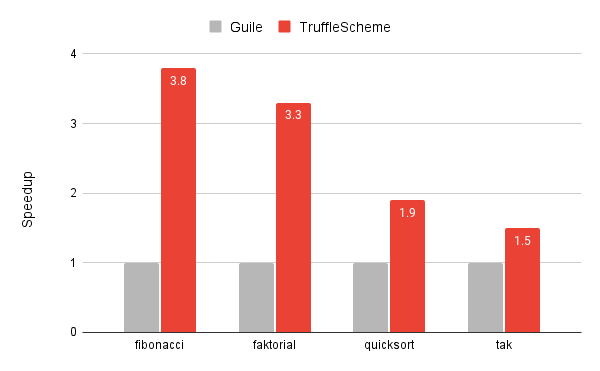
\includegraphics[width= 1\textwidth]{images/guile-chart.png}
%     \caption{Srovnání výkonosti Guile implementace s~TruffleScheme implementací}
%     \label{fig:guile-benchmark}
% \end{figure}

Na obrázku~\ref{fig:grouped-benchmark} jsou zobrazeny výsledky měření. Graf zobrazuje, zda je TruffleScheme rychlejší, či pomalejší v~porovnání s~Guile. Například TruffleScheme je 3.6krát rychlejší při výpočtu n-tého čísla Fibonacciho řady ve srovnání s Guile. Obecně vyššího výkonu dosahuje TruffleScheme ve všech benchmarcích. Primárním důvodem je způsob, jakým obě implementace nakládají s~daty, které je možné získat z~běhu programu. Zatímco TruffleScheme (a obecně jazyky implementované nad platformou GraalVM) využívá co nejvíce dat z~běhu programu, Guile nepoužívá žádná data. Výjimkou je počet volání jednotlivých procedur, aby bylo možné rozhodnout, zda je procedura vhodným kandidátem k~JIT kompilaci~\cite{guile3-jit}. Takovému typu JIT překladače se často říká \textit{Template-Based JIT~Compiler}. Jelikož pro přeložení do strojového kódu není potřeba žádná analýza mezikódu, je překlad výrazně rychlejší v~porovnání s~překladačem Graal. Naopak, jak je možné vidět z~výsledku měření, výsledný strojový kód není tak efektivní, jelikož nedokáže provádět tak sofistikované optimalizace. 


\subsection{Srovnání s~Racket implementací}
Racket (dříve známý jako MzScheme) je považován za potomka jazyka Scheme. Jeho syntaxe je tak téměř identická s~jazykem Scheme. Podobně jako Guile, Racket také obsahuje virtuální stroj včetně JIT překladače, nicméně během JIT kompilace využívá data z~běhu programu, čímž se ještě více podobá implementaci TruffleScheme. Pro měření byla použita Racket verze 8.8, což je nejaktuálnější verze dostupná v~době psaní diplomové práce. Jak je možné vidět z~grafu~\ref{fig:grouped-benchmark}, rychlosti jednotlivých implementací jsou daleko podobnější než v~předchozím srovnání. Primárním důvodem je již zmíněný JIT překladač, který v~obou implementacích využívá data z~běhu programu.  


Největší zrychlení je možné vidět v~benchmarku \textit{faktorial}, kde je TruffleScheme 2krát rychlejší. Hlavním důvodem je optimalizace koncové rekurze, která v~implementaci TruffleScheme eliminovala volání rekurzivní procedury, tudíž eliminovala režii spojenou s~voláním procedury. Racket pravděpodobně nerozlišuje mezi optimalizací na koncovou rekurzi a optimalizací na koncové volání, jelikož vygenerovaný strojový kód obsahuje volání rekurzivní procedury. 


\begin{figure} [h]
    \centering
    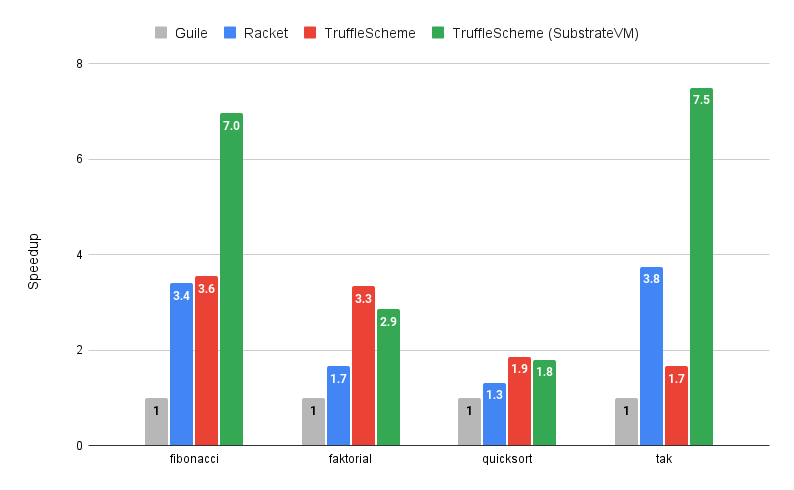
\includegraphics[width= 1\textwidth]{images/benchmark-grouped.png}
    \caption{Výkonnostní srovnání Guile, Racket a TruffleScheme. TruffleScheme je možné buďto spustit nad JVM, nebo využít technologii SubstrateVM}
    \label{fig:grouped-benchmark}
\end{figure}


Z~grafu je dále možné vidět, že benchmark \texttt{tak} je výrazně pomalejší v~porovnání s~Racket implementací. Možný důvod je vidět na obrázku \ref{fig:graal-ir}, kde je vizualizována interní reprezentace (Graal IR), která se využívá k~určení, jaké optimalizace byly na zdrojový kód aplikovány v~různých fázích překladu. V~tomto případě obrázek reprezentuje tělo metody \texttt{tak} (viz zdrojový kód \ref{tak-impl}), kde je možné vidět, že koncová rekurze byla transformována na smyčku (uzel 362 reprezentuje začátek smyčky, uzel 2402 ukončení smyčky a uzel 2405 ukončení jedné iterace). Dále je možné vidět, že překladač nebyl schopen eliminovat boxování argumentů (např. uzly 2681, 2682, 2683), které jsou následně uloženy v~poli typu \texttt{Object[]} a předány k~rekurzivnímu volání. Právě tyto uzly jsou důvodem, proč je benchmark pomalejší. Eliminace těchto uzlů ale není v~tuto chvíli možná, jelikož se jedná o~omezení JVM. 


Problém s~boxováním lze ale vyřešit pomocí technologie \textit{SubstrateVM}. Interprety jazyků implementovaných nad platformou GraalVM mohou být přeloženy přímo do strojového kódu, tudíž není potřeba JVM pro jejich spuštění. Jedná se o~tzv. \textit{ahead-of-time kompilaci} (AOT), jejímž výsledkem je tzv.~\textit{native-image}. JVM je zde nahrazeno SubstrateVM obsahující komponenty, které jsou běžně součástí běhového prostředí JVM, jako např. deoptimalizátor, správce paměti nebo správce vláken. Tyto komponenty jsou k~dispozici během překladu, a tudíž jsou součástí výsledného strojového kódu. Jelikož byly tyto komponenty tvořeny pro interpretaci jazyků, odstraňují některá omezení JVM. Jedním z~nich je výše zmíněné boxování argumentů při volání procedur. Na grafu~\ref{fig:grouped-benchmark} je možné vidět srovnání implementace TruffleScheme, která je přeložena do strojového kódu a využívá tedy technologii SubstrateVM, s ostatními implementacemi. Benchmarky založené na rekurzivním voláním procedur (výpočet n-tého čísla Fibonacci řady a Takeuchi funkce) dosáhly výrazného zrychlení, jelikož v~obou případech bylo eliminováno boxování jednotlivých argumentů.  


\begin{listing} [h]
    \begin{minted}{scheme}
        (define tak
          (lambda (x y z)
            (if (not (< y x))
                z (tak (tak (- x 1) y z)
                   (tak (- y 1) z x)
                   (tak (-  1) x y)))))
    \end{minted}
    \caption{Implementace Takeuchi funkce v~jazyce Scheme}
    \label{tak-impl}
\end{listing}


% \begin{figure} 
%     \centering
%     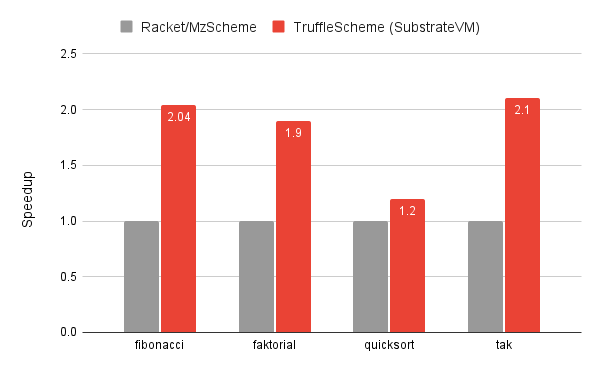
\includegraphics[width= 1\textwidth]{images/substratevm-chart.png}
%     \caption{Výkonnostní srovnání Racket s TruffleScheme, využívající technologii SubstrateVM }
%     \label{fig:substrateVM-benchmark}
% \end{figure}


\begin{figure} [h]
    \centering
    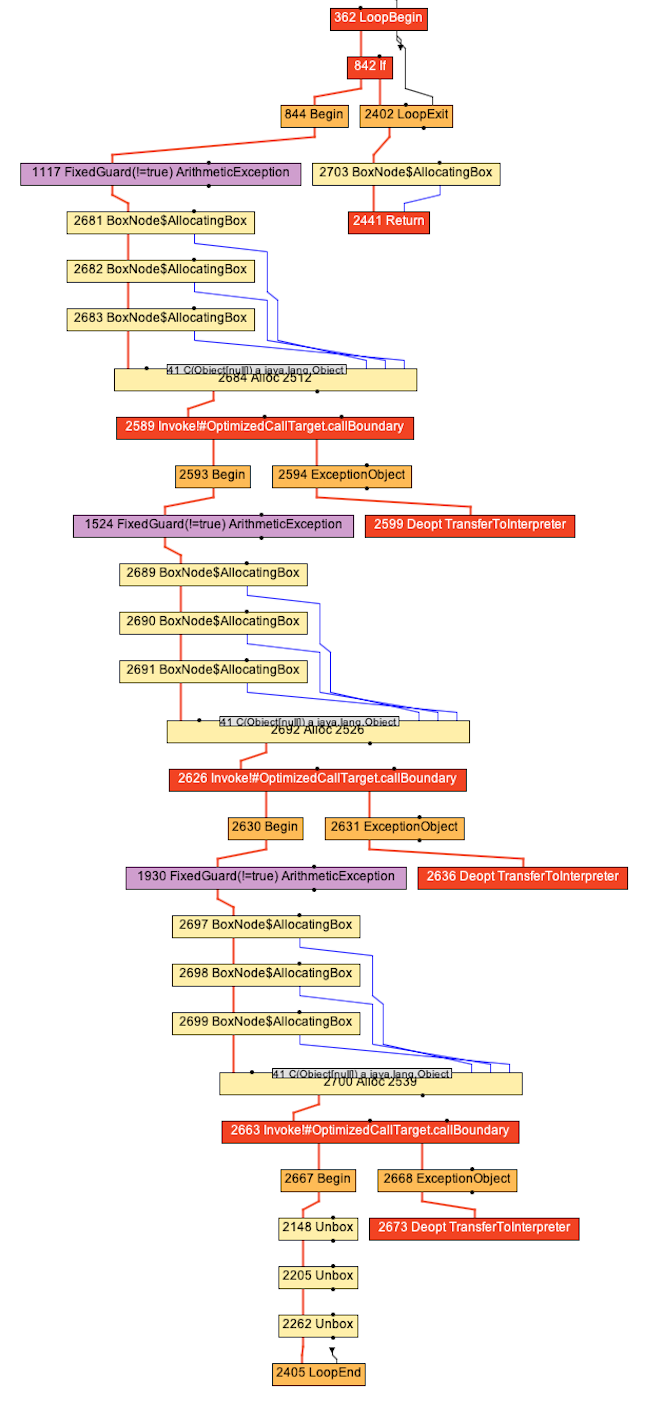
\includegraphics[width= 0.8\textwidth, height=1.48\linewidth]{images/graalIR.png}
    \caption{Interní reprezentace (Graal IR) těla procedury \texttt{tak}}
    \label{fig:graal-ir}
\end{figure}




%% Závěry práce. V jazyce práce a anglicky. Text pro jiný než
%% nastavený jazyk práce (nepovinným parametrem language makra
%% \documentclass, výchozí český) se zadává použitím makra s uvedením
%% jazyka jako nepovinného parametru.
\begin{kiconclusions}
Cílem práce bylo vytvořit interpret funkcionálního jazyka na platformě GraalVM. Vznikl tak TruffleScheme, interpret jazyka Scheme, který svou rychlostí ve vybraných benchmarcích překonává implementace jako Guile nebo Racket. TruffleScheme je jedna z~prvních implementací na platformě GraalVM, která poskytuje optimalizaci koncových volání a optimalizaci pro koncovou rekurzi bez negativního dopadu na rychlost interpretu. Naopak implementace optimalizace pro koncovou rekurzi interpret výrazně zrychlila, jelikož eliminovala volání rekurzivní procedury, čímž odstranila režii spojenou s~jejím voláním. 

Ačkoliv TruffleScheme není kompletní implementací jazyka Scheme, výsledky benchmarků dokazují, že platforma GraalVM je nejen vhodná pro kompletní implementaci jazyka Scheme, ale i pro ostatní funkcionální jazyky. TruffleScheme je v~průměru 2.6krát rychlejší v~porovnání s~Guile implementací a 1.2krát rychlejší v~porovnání s~Racket implementací. Nejlepších výsledků bylo dosaženo při použití technologie SubstrateVM, kde TruffleScheme je v~průměru 4.7krát rychlejší než Guile implementace a 1.8krát rychlejší než Racket implementace. 


Dalším důležitým aspektem implementace byla podpora interoperability s~dalšími jazyky dostupnými na platformě GraalVM, čímž TruffleScheme umožňuje polyglotní programování. Pro dosažení tohoto cíle bylo nutné navrhnout generické aplikační rozhraní, které umožňuje například vyhodnocovat kód cizích jazyků nebo číst vazby definované v~globálním prostředí těchto jazyků. Rychlost této implementace byla záměrně ponechána pro potenciální budoucí zlepšení. 

Cílem tohoto textu bylo nejprve teoreticky vysvětlit, na jakém principu platforma GraalVM spolu s~frameworkem Truffle pracuje, a poté popsat implementaci základních prvků jazyka. Text mimo jiné obsahuje mnoho implementačních detailů, včetně konkrétních příkladů, které mohou sloužit jako podklad pro budoucí vývoj jazyků na platformě GraalVM. 
\end{kiconclusions}

\begin{kiconclusions}[english]
This thesis aimed to develop a functional language interpreter on the GraalVM platform. The result is TruffleScheme, which is a Scheme language interpreter that surpasses implementations such as Guile or Racket in selected benchmarks. TruffleScheme is one of the first implementations on the GraalVM platform that supports Tail Call and Tail Recursive optimizations without negatively affecting the speed of the interpreter. Conversely, the implementation of Tail Recursive optimization has significantly sped up the interpreter by eliminating the recursive call, thus eliminating the overhead associated with the call.

Although TruffleScheme is not a complete implementation of the Scheme language, the benchmark results show that the GraalVM platform is not only suitable for a complete implementation but also for other functional languages. TruffleScheme is on average 2.6 times faster than the Guile implementation and 1.2 times faster than the Racket implementation. The best results have been achieved using SubstrateVM, where TruffleScheme is on average 4.7 times faster than the Guile implementation and 1.8 times faster than the Racket implementation.

Another important aspect of this thesis was to support interoperability with languages implemented on the GraalVM platform, which would enable polyglot programming. To achieve this goal, it was necessary to design and implement a new generic API that allows, for example, to evaluate the code of foreign languages or read bindings defined in the global environment of these languages. The speed of this implementation was defined as an explicit non-goal that was intentionally left for potential future improvements.

The goal of this text was first to explain the theoretical principles on which the GraalVM and Truffle framework works and then to describe the implementation of basic elements of the language. This text contains many implementation details, including examples, which can serve as a solid foundation for further language development on the GraalVM platform.
\end{kiconclusions}

%% Přílohy obsahu textu práce, za makrem \appendix.
\appendix

% \section{První příloha}
% Text první přílohy

% \section{Druhá příloha}
% Text druhé přílohy

%% Obsah elektronických dat. Poslední příloha. Upravte podle vlastní
%% práce!
\section{Obsah elektronických dat} \label{sec:ObsahData}

Elektronická data odevzdaná v systému katedry mají následující strukturu:

\begin{description}

\item[\texttt{text/}] \hfill \\
  Adresář s textem práce ve formátu PDF, vytvořený s~použitím
  závazného stylu KI PřF UP v~Olomouci pro závěrečné práce, včetně
  všech (textových) příloh, a~všechny soubory potřebné pro
  bezproblémové vytvoření PDF dokumentu textu (případně v~ZIP
  archivu), tj.~zdrojový text textu a příloh, vložené obrázky, apod.

\item[\texttt{README.md}] \hfill \\
  Instrukce pro sestavení a~spuštění interpretu \textsc{TruffleScheme}, včetně
  všech požadavků pro jeho bezproblémový provoz.

\item[\texttt{bin/}] \hfill \\
  Binární soubory pro spuštění interpretu pro operační systém Linux (amd64) a macOS (aarch64). Dále složka obsahuje soubor \texttt{scm-component.jar}, který je možné využít pro instalaci interpretu jako komponenty pomocí Graal Updater. 

\item[\texttt{src/}] \hfill \\
  Kompletní zdrojový kód interpretu \textsc{TruffleScheme}, rovněž dostupný na \url{https://github.com/horakivo/TruffleScheme}.

\item[\texttt{examples}] \hfill \\
  Zdrojové kódy, které byly použity pro srovnání rychlosti s ostatními implementacemi v~kapitole \ref{benchmark-chapter} této práce.

\end{description}

% U~veškerých cizích obsažených materiálů jejich
% zahrnutí dovolují podmínky pro jejich veřejné šíření nebo přiložený souhlas
% držitele práv k užití. Pro všechny použité (a~citované) materiály,
% u~kterých toto není splněno a~nejsou tak obsaženy, je uveden
% jejich zdroj, např.~webová adresa, v~bibliografii nebo textu práce
% nebo souboru \texttt{README.md}.

%% -------------------------------------------------------------------

%% Sazba volitelného seznamu zkratek, za přílohami.
%% \printglossary

%% Sazba povinné bibliografie, za přílohami (případně i za seznamem
%% zkratek). Při použití BibLaTeXu použijte makro
%% \printbibliography. jinak prostředí thebibliography. Ne obojí!

%% Sazba i v textu necitovaných zdrojů, při použití
%% BibLaTeXu. Volitelné.
\nocite{*}
%% Vlastní sazba bibliografie při použití BibLaTeXu.
\printbibliography

%% Bibliografie, včetně sazby, při NEpoužití BibLaTeXu.
% \begin{thebibliography}{9}
%\bibitem{kniha2} \uppercase{Hawke}, Paul. NanoHttpd: Light-weight HTTP server designed for embedding in other applications. GitHub [online]. 2014-05-12. [cit. 2014-12-06]. Dostupné z: \url{https://github.com/NanoHttpd/nanohttpd}
%
%\bibitem{jeske13} \uppercase{Jeske}, David; \uppercase{Novák}, Josef. Simple HTTP Server in \csharp: Threaded synchronous HTTP Server abstract class, to respond to HTTP requests. CodeProject: For those who code [online]. 2014-05-24. [cit. 2014-12-06]. Dostupné z: \url{http://www.codeproject.com/Articles/137979/Simple-HTTP-Server-in-C}
%
%\bibitem{uzis2012} \uppercase{ÚSTAV ZDRAVOTNICKÝCH INFORMACÍ A STATISTIKY ČR}. Lékaři, zubní lékaři a farmaceuti 2012 [online]. Praha 2, Palackého náměstí 4: Ústav zdravotnických informací a statistiky ČR, 2012 [cit. 2014-12-06]. ISBN 978-80-7472-089-5. Dostupné z: \url{http://www.uzis.cz/publikace/lekari-zubni-lekari-farmaceuti-2012}
% \end{thebibliography}

%% Sazba volitelného rejstříku, za bibliografií.
\printindex

\end{document}

%%% Local Variables:
%%% mode: latex
%%% TeX-master: t
%%% End:
